\documentclass[doktyp=marbeit,fontsize=12pt,sprache=english,hausschrift=true]{TUBAFarbeiten}

% packages
\usepackage{abstract}
\usepackage{amsmath}
\usepackage[ngerman]{babel}
\usepackage{blindtext}
\usepackage{caption}
\usepackage{capt-of}
\usepackage{calc}
\usepackage{cite}
\usepackage{enumitem}
\usepackage[T1]{fontenc}
\usepackage{floatrow} % rows of table and pictures
\usepackage{graphicx}
\usepackage{gensymb}
\usepackage[utf8]{inputenc}
\usepackage{makeidx}
\usepackage[fleqn]{mathtools} % mathtools und links buendig machen
\usepackage{subcaption}
\usepackage{listings}
\usepackage{tabu}
\usepackage{spreadtab}
\usepackage{pgfplots}
\usepackage{xcolor}

\definecolor{darkgreen}{RGB}{65,117,5}
\definecolor{darkred}{RGB}{208,2,27}

\definecolor{plotblue}{HTML}{4A90E2}
\definecolor{plotorange}{HTML}{F5A623}
\definecolor{plotdarkblue}{HTML}{000FFF}
\definecolor{plotdarkorange}{HTML}{FF5200}

\lstset{language=C++,
    keywordstyle=\color{blue}\bfseries,
    commentstyle=\color{green},
    stringstyle=\ttfamily\color{red!50!brown},
    basicstyle=\linespread{0.8}\ttfamily,
    numbers=left,
    stepnumber=1,
    showstringspaces=false}
\lstset{literate=%
   *{0}{{{\color{red!20!violet}0}}}1
    {1}{{{\color{red!20!violet}1}}}1
    {2}{{{\color{red!20!violet}2}}}1
    {3}{{{\color{red!20!violet}3}}}1
    {4}{{{\color{red!20!violet}4}}}1
    {5}{{{\color{red!20!violet}5}}}1
    {6}{{{\color{red!20!violet}6}}}1
    {7}{{{\color{red!20!violet}7}}}1
    {8}{{{\color{red!20!violet}8}}}1
    {9}{{{\color{red!20!violet}9}}}1
}

% Images with mathcha.io 
\usepackage{tikz}
\usetikzlibrary{fadings}
\usepackage{mathdots}
\usepackage{yhmath}
\usepackage{cancel}
\usepackage{color}
\usepackage{siunitx}
\usepackage{array}
\usepackage{multirow}
\usepackage{amssymb}
\usepackage{gensymb}
\usepackage{tabularx}
\usepackage{booktabs}
% Images end


\usepackage{subscript} % tief stellen
%\usepackage[square]{natbib}
\usepackage{setspace}
\renewcommand{\baselinestretch}{1.5}

\usepackage{mathtools}
\newcommand{\colvecxx}[2]{\left(\begin{array}{c} #1 \\ #2 \end{array}\right)}
\newcommand{\colvecxxx}[3]{\left(\begin{array}{c} #1 \\ #2 \\ #3 \end{array}\right)}
\newcommand{\colvech}[3]{\left(\begin{array}{c} #1 \\ #2 \\ #3 \\ 1\end{array}\right)}

\newcommand{\rowvecxx}[2]{\left(\begin{array}{cc} #1 & #2 \end{array}\right)^T}
\newcommand{\rowvecxxx}[3]{\left(\begin{array}{ccc} #1 & #2 & #3 \end{array}\right)^T}

\newcommand{\lnorm}[1]{\lVert#1\rVert}

\DeclareMathOperator{\arctantwo}{arctan2}

\DeclarePairedDelimiter{\ceil}{\lceil}{\rceil}
\DeclarePairedDelimiter{\floor}{\lfloor}{\rfloor}
\DeclarePairedDelimiter{\abs}{\lVert}{\rVert} % definiere absoluten betrag

% https://tex.stackexchange.com/questions/9466/color-underline-a-formula
\def\mathunderline#1#2{\color{#1}\underline{{\color{black}#2}}\color{black}}

% https://tex.stackexchange.com/questions/6850/table-and-figure-side-by-side-with-independent-captions
% Table float box with bottom caption, box width adjusted to content
% \newfloatcommand{capbtabbox}{table}[][\FBwidth]
% https://tex.stackexchange.com/questions/101980/table-and-figure-side-by-side-with-table-caption-above-figure-caption-below
% \newfloatcommand{capbtabbox}{table}[\captop][\FBwidth]
\newfloatcommand{btabbox}{table}[][\FBwidth]


\usepackage[acronym,toc]{glossaries}
\glstoctrue%

\newglossary[nlg]{symbols}{nls}{nlo}{Symbol Definition}
\makeglossaries%
\loadglsentries{chapter00/acronyms}
\loadglsentries{chapter00/definitions}
\loadglsentries{chapter00/symbols}

% tubaf zeugs
\TUBAFFakultaet{Fakultaet für Mathematik und Informatik}
\TUBAFInstitut{Institut für Informatik}
\TUBAFLehrstuhl{Lehrstuhl für virtuelle Realitaet und Robotik}
\TUBAFTitel{Sensor Localization of Range Data using a Feature based Registration}
\TUBAFBetreuer{Prof.\ Dr.\ Bernhard Jung}
\TUBAFKorrektor{Dipl-Ing. Mark Sastuba}
\TUBAFAutor[J. Toth]{Jonas Toth}
\TUBAFStudiengang{Angewandte Informatik}
\TUBAFMatrikel{57319}
%\TUBAFAnmeldeDatum[2017-02-8]{8. Februar 2017}
\TUBAFDatum{25. September 2019}


\setcounter{tocdepth}{3}
\setcounter{secnumdepth}{3}

% \makeindex

\usepackage[pdftex, unicode, hidelinks,
            pdfproducer={Latex with hyperref},
            pdfcreator={pdflatex}]{hyperref}
\hypersetup{colorlinks=false,
            citecolor=black,
            filecolor=black,
            linkcolor=black,
            urlcolor=black,
            linktoc=all}


% start the content
\begin{document}

\maketitle
\TUBAFErklaerungsseite%

\begin{abstract}
\noindent
Features --- special identifiable elements --- and their recognition between different images play an important role in computer vision to solve tasks like visual odometry, place and object recognition or global localization.
Methods for these areas are established and implemented for common mobile devices and robots.
Even though depth data processing is omnipresent for robotic systems, feature detectors for salient, recognizable segments of such pointclouds are not an established method for reliable and robust localizations without prior knowlegde.

This work proposes depth image processing steps to utilize feature detectors and descriptors for color images on depth data.
In order to apply the algorithms SIFT, SURF, ORB and AKAZE on depth images, they are converted into dervied feature images that encode the local geometry of the measured environment.
Multiple possible transformations of the depth data, from the already proposed Bearing-Angle image to measures of curvature and finally the novel Flexion image, are developed, analyzed and evaluated with respect to, among other things, keypoint stability and discrimination potential of the descriptors.
The aspects keypoint count, size, response, the matching distance between true and false positives and additional measures like precision, recall and informedness are determined for four experimental datasets.
They consist of a synthetic scene, a underground mining environment, an office scene and LiDAR scans.
In addition, the impact of filtering the depth data with edge-preserving filters is analyzed on the outcome.

All experiments indicate a consistently better performance of the Flexion image compared to the Bearing-Angle image and proof that SIFT and AKAZE are suitable as feature detectors and descriptors whereas SURF and ORB are not.
This insight is underlined with the computation of a visual odometry benchmark.
The research forms a solid foundation to further develop the use of classical computer vision algorithms on Flexion images to accomplish feature-related tasks with depth data.
\end{abstract}

\newpage
\begin{abstract}
Sehr wichtige Arbeit
\end{abstract}

\newpage

\pagenumbering{roman}
\tableofcontents
\newpage

\setlength{\glsdescwidth}{0.82\linewidth}
\setlength{\glspagelistwidth}{0.18\linewidth}
\printglossary[type=\acronymtype,style=super,nonumberlist,nopostdot]%
\newpage

\printglossary
\newpage

\printglossary[type=symbols,style=super,nopostdot]%
\glsaddallunused[symbols]
\newpage


\pagenumbering{arabic}
\newpage

\section{Introduction}
Global and local pose estimation is a common problem solved in robotics.
Visual odometry\cite{he_tvc2019} and \gls{feature}-based localization\cite{sattler_cvpr2018} are established solutions and a lot of research went into these various aspects of this field.
Additionally, the use of depth sensors increased with their availability and fast integration into robotic systems.
This naturally leads to the task of exploiting the depth information for problems like localization and mapping, which at their core require a way to align multiple pointclouds to each other.

One dominant algorithm to solve this problem is \acrshort{icp} (\acrlong{icp})\cite{besl_pami1992}.
It has various characteristics and limitations that require an initial estimate for the relative pose between pointclouds\cite{rusinkiewicz_ieee2001}.
Loop closure in \acrshort{slam} (\acrlong{slam})\cite{ho_ros2006}, global localization and place recognition\cite{sattler_2011} can not rely on such an initial estimate.
Those problems are commonly solved with a \gls{feature}-based approach to detect salient points in color images that are recognized in optical sensor data.
Detecting salient points in an image and describing the local neighbourhood in a recognizable manner is at the core of many solutions of computer vision related problems and a well researched topic\cite{andersson_2016}.

The context of this thesis is research of robotic systems in underground mining environments.
It is common to have detailed \acrshort{LIDAR} scans of the whole mine, which is a part of mine surveying.
Bad lighting conditions challenge the classical optical systems and algorithms to achieve global localization.
Other techniques, like GPS, are outright impossible to use.

The aim of this thesis is to develop the foundation to process depth sensor data and \acrshort{LIDAR} scans, such that well developed computer vision algorithms become applicable to depth and range data.
Each depth image is first converted into a derived feature image that visualizes the geometrical relationship between neighbouring, three-dimensional points.
The \gls{feature} detectors and descriptors are then run on the feature image to detect salient point constellations consistently.

The proposed feature images have different visual characteristics than color images.
For successfull usage of \gls{feature}-based depth data registration, the detected keypoints need to be stable between multiple views and the descriptors for each keypoint must discriminate between different sections.
Researching the properties of both the keypoints and the descriptors for common state-of-the-art algorithms is therefore mandatory work before solving more complex tasks like global localization, that use \glspl{feature} at their core.
The findings shall be used in a simple visual odometry experiment to demonstrate principal applicability of the final result.

The main contribution of this thesis is a novel way to convert depth data into a derived feature image and the analysis of the performance of state-of-the-art keypoint detectors and descriptors on this derived image.
All developed tools can be reused as both library code and executable binary to create such images and run \gls{feature} algorithms on them.
Both the qualitative and quantitative findings will build an empirical foundation on developing this approach further for more complex tasks such as place recognition, global localization in a known environment and visual odometry with the novel feature images as input.

The structure of this thesis is based on the necessary steps to extract visual keypoints from converted depth images.
Section~\ref{sec:related_work} introduces the related work on state-of-the-art algorithms for pointcloud registration and \gls{feature} performance comparisons.
Necessary foundational knowledge on depth sensors and the math of modeling their data is presented in Section~\ref{sec:fundamentals}.
Additionally, it gives a high level introduction on keypoint detectors and descriptors and how their performance can be evaluated.
Section~\ref{sec:image_processing} describes the novel depth data processing, starting with edge-preserving filtering followed by conversion to feature images and finally explaining the evaluated \gls{feature} detection and description algorithms.
The proposed pipeline is evaluated in Section~\ref{sec:experiments}, describing the approach and metrics.
Section~\ref{sec:results} presents and discusses the results.
Finally, Section~\ref{sec:conclusion} concludes the work and proposes further research areas to develop this new approach for depth image registration.

\newpage

\section{Related Work}
Scaramuzza's\cite{scaramuzza_iros2007} work on calibrating the extrinsic of a \acrshort{LIDAR} scanner to a camera is the introduces the \gls{bearing-angle-image}.
The conversion of range data to a derived visual representation format allows manual selection of corresponding corners, edges and other salient regions in both the color image and the \gls{bearing-angle-image}.
Minimizing the reprojection error for the selected points allows to compute a relative rotation and translation between both modalities.
Lin et al.\cite{lin_easp2017} apply the \acrshort{surf}\cite{bay_eccv06} feature detector on \glspl{bearing-angle-image}.
The keypoints detected in multiple range images allow to reconstruct the relative pose between dense pointclouds.
They additionally compare the performance of this registration to state-of-the-art \acrshort{icp} (\acrlong{icp}) algorithms.
They conclude, that the \acrshort{icp} has higher precision but execution speed is drastically improved when using the \gls{bearing-angle} based pose as initial state.
To the best of the author's knowledge, no other work includes the use of \glspl{bearing-angle-image}.

\subsection{Pointcloud Registration}

The cited publications are novel approaches to a well researched and developed area --- pointcloud registration.
Range sensors produce a set of points and one natural task is to determine the relative transformation between two such sets.
This task has many applications in photogrammetry, robotics and engineering.

\acrshort{icp}, originally formulated by Besl\cite{besl_pami1992} is a robust and easy to implement algorithm to achieve this registration.
At its core is the assignment of point correspondences between both sets, calculating a relative pose that results in the lowest distance between the choosen points and evaluating the disparity of both pointclouds.
The mismatch of the pose is iteratively reduced by finding better correspondences using the distance between the points of the pointclouds as error metric.
This basic approach received multiple improvements with the generalized \acrshort{icp}\cite{segal_2009,korn_2014} providing a fully probabilistic formulation.
\acrshort{icp} provides a 6 \acrlong{DoF} (\acrshort{DoF}) registration consisting of a rotation and translation.
Convergence or an upper bound of the error is not guaranteed and in general relies on a good initial estimate of the relative pose of both pointclouds, rendering it useless for global registration problems without prior knowledge.
Failure to converge on a relative pose can happen both due to a bad initial pose or not corresponding pointclouds.

A different approach to pointcloud registration is provided by the \acrlong{NDT} (\acrshort{NDT}) algorithm proposed by Biber and Straßer\cite{biber_iros2003}.
It works without explicit correspondences between both pointclouds.
First, the range image is subdivided into cells.
Each cell approximates a normal distribution of the probability of measuring a point at a position within the cell.
Registering a second pointcloud is a matter of maximizing the likelihood that the pointcloud is measured in the reference pointcloud under a given pose.
The normal distributions are differentiable and classical numerical algorithms, like Newton's algorithm, can be used for the maximization.

Myronenko and Song\cite{myronenko_ieee2010} proposed the \acrlong{CPD} (\acrshort{CPD}) algorithm.
Similar to \acrshort{NDT} the algorithm utilizes probabilistic methods to achieve the registration.
A pointcloud is modelled with a \acrlong{GMM} (\acrshort{GMM}) defined through multiple centeroids and their variances.
Again, alignment of two pointclouds means the maximal probability of the data points under the \acrshort{GMM}.
In iterative refinement steps of the relative pose the centeroids of the \acrshort{GMM} are enforced to move in topological consistent fashion, hence coherent point drift.
The review articles~\cite{bellekens_ambient2014,pomerleau_2015} introduce state-of-the-art pointcloud registration algorithms both in general and for robotic applications.

Feature-like algorithms are uncommon, but some approaches exist in the literature.
Elbaz et al.\cite{elbaz_cvpr2017} extract subsets of a pointcloud, analyze its main directional components using a principal component analysis and synthesize a depth map for these patches.
A deep neural network based auto-encoder computes a low-dimensional descriptor for each patch.
Registration of pointclouds is achieved by matching these descriptors followed by a conventional fine-tuning step.

Steder et al.\cite{steder_robot2010} proposed an interest point detector for range images.
The image's curvature is analyzed by first smoothing with a Gaussian and then computing the second derivatives of the range data.
High curvature is used for saliency, but special points on an edge and regions of occlusion are filtered out first.
Interest points must succeed a certain threshold to be selected.
The selected points are used to calculate transformations between different range images and each potential transformation is scored by the reprojection error.

% \subsection{Multi-Modal Sensor Registration}

% \begin{itemize}
    % \item Kinect Fusion uses ICP\cite{newcombe_ismar2011}
    % \item dense visual odometry uses photometric error of all image information, instead of sparse features like SIFT\cite{kerl_icra2013}, photo consistency assumption -> the brightness of a point stays constant between two camera poses.
    % \item multi-cue photometric registration\cite{corte_icra2018}
    % \item image-to-geometry mapping based on correlation\cite{corsini_cgf2009}
    % \item laser scan registration based on panorama pictures from coregistered camera or intensity images\cite{alba_isprs2012}
    % \item SIFT realistic rendering to match images with pointclouds\cite{sibbing_3dv2013}
    % \item Synthetic views from dense pointcloud intensity images, matched with camera maximizing normalized mutual information\cite{wolcott_iros2014,zhao_icra2016}
    % \item laser scan registration using planar patches and image data\cite{dold_iaprs2006}
% \end{itemize}

\subsection{Feature Algorithm Comparison}

Keypoint detectors and feature descriptors are a well established technique in the computer vision community.
They provide a way to detect salient regions of a gray-scale image that can be consistently detected between different views of a scene.
The breakthrough development is Lowe's SIFT\cite{lowe_ijcv04} algorithm.
The early benchmark\cite{mikolajczyk_pami2005} of SIFT to other classical algorithms, like the Harris corner detector\cite{harris_1988}, demonstrated the strong performance of SIFT.
Since the early 2000s more work on improving upon SIFT in terms of performance, compute requirements and diverse applications lead to more competitors like SURF\cite{bay_eccv06}, ORB\cite{rublee_iccv11} and AKAZE\cite{alcantarilla_bmva13}.
A recent comparison between those modern, well established algorithms by Andersson and Reyna Marquez\cite{andersson_2016} still puts SIFT as a top-performer, with AKAZE\cite{alcantarilla_bmva13} yielding similar but slightly less accurate results.
ORB\cite{rublee_iccv11} on the other hand is less accurate but due to its lower computational cost still a viable option, especially for mobile applications.
The use of classical feature descriptors and template based matching for different modalities, like thermal imaging, is evaluated by Gesto-Diaz et al.\cite{gesto-diaz_2017}.
They conclude that the detectors result in many correct matches within on modality.
Correct intermodal matching on the other hand is harder and depends on the modalities used.
They note that combining thermal and range images yield the worst performance regardless of the used registration technique.
The result is encouraging that algorithms like SIFT\cite{lowe_ijcv04} are not bound to color images but can be used in scenarios with vastly different appearance.
It also motivates to search for better ways to process range data with feature based matching.

\newpage

\section{Fundamentals}

This section introduces the relevant principles used to create and evaluate the novel approach on depth data processing.

\subsection{Depth Sensors}

Depth sensors play an increasingly important role in modern robotic applications.
They give a robot a fast mean to detect obstacles and locate itself in its environment.
The following paragraphs describe the underlying sensing principles\cite{blais_2003} for the depth sensors commonly used in mobile robotic applications.

\subsubsection{Structured-Light Depth Sensors}

\begin{figure}[H]
    \centering
    \begin{subfigure}[t]{0.45\textwidth}
        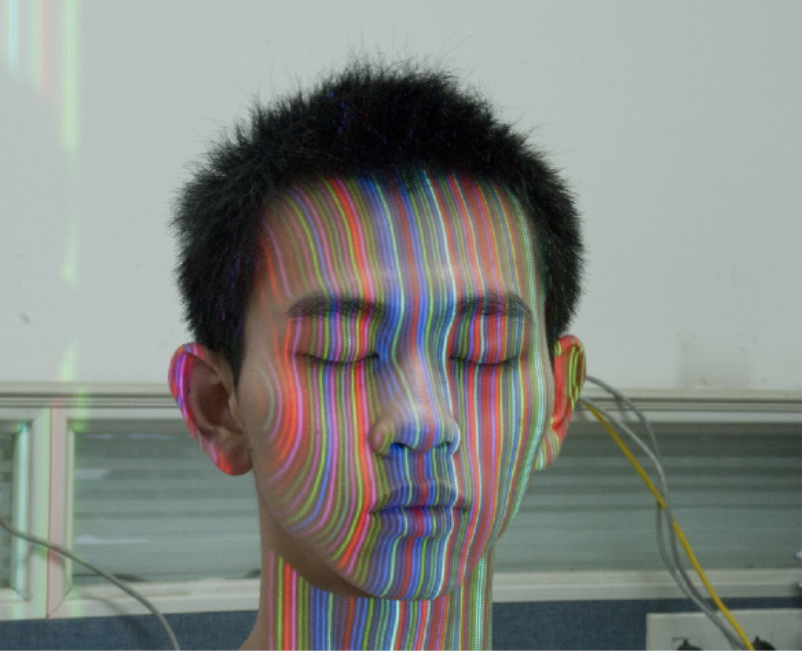
\includegraphics[width=\textwidth]{chapter03/img/depth_pattern_face.png}
        \caption{Visible structured light pattern}
    \end{subfigure}
    \begin{subfigure}[t]{0.45\textwidth}
        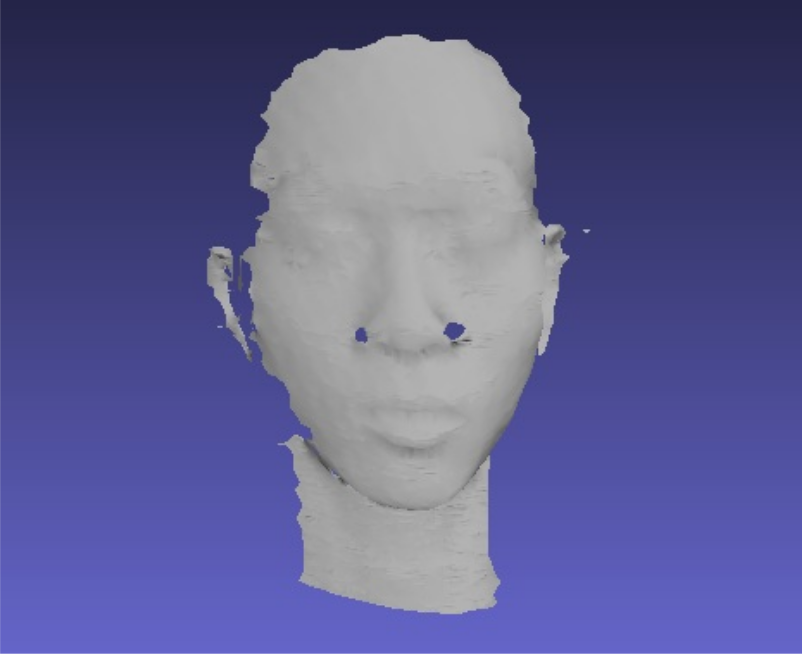
\includegraphics[width=\textwidth]{chapter03/img/depth_face_reconstructed.png}
        \caption{Reconstructed result}
    \end{subfigure}
    \caption[Demonstration of structured-light depth sensors]{\emph{Demonstration of structured-light depth sensors.} One way to reconstruct depth information are structured light depth sensors. A predefined light pattern is projected into space. As the photons reflect from obstacles at different distances relative to the observer, the light pattern appears transformed. This deformation is used to reconstruct the geometry of the objects. The light emitted is usually not visible to humans as infrared light sources and cameras are commonly used in robotic applications.The images are taken from \cite{sl_depthsensor_calibration}.}\label{fig:sl_face}
\end{figure}
Structured-light depth sensors project a known light pattern into space and optically sense the reflection.
The pattern appears distorted from a viewpoint different than the projector due to the shape of the reflecting object.
Figure~\ref{fig:sl_face} provides an example for structured-light sensing using visible light.
Stripes and grids of lines or points are common for sensors in robotic applications, such as the Kinectv1 and Intel RealSense\cite{intel_realsense} sensors.
Viewing the projected patterns from multiple viewpoints allows triangulation to recover the depth information.
Mobile robotic depth sensors achieve framerates of 30fps or more.
The projected pattern should not interfere with other optic devices leading to infrared light.

\subsubsection{\acrlong{ToF}-cameras (\acrshort{ToF})}

\begin{figure}[H]
    \centering
    \begin{subfigure}[t]{0.45\textwidth}
        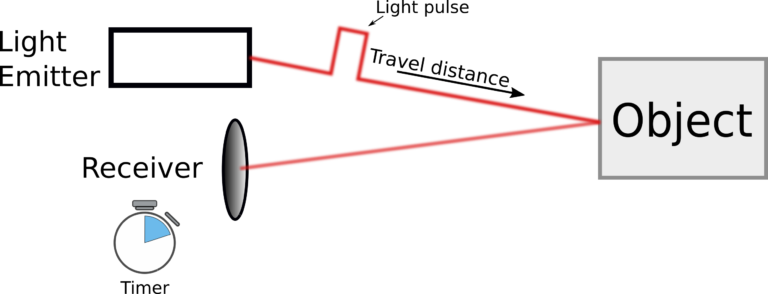
\includegraphics[width=\textwidth]{chapter03/img/tof_traveltime_original.png}
        \caption{One way to measure the time-of-flight for photons is to emit a light pulse and measure the roundtrip time until the reception of the reflection.}\label{fig:tof_roundtrip}
    \end{subfigure}\quad
    \begin{subfigure}[t]{0.45\textwidth}
        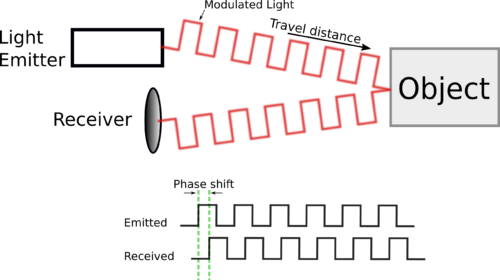
\includegraphics[width=\textwidth]{chapter03/img/tof_phase_shift_original.png}
        \caption{The second, more recent approach is measuring the phase-shift of photons relative to the light source. This allows a continously emitting light source.}\label{fig:tof_phase_shift}
    \end{subfigure}
    \caption[Illustration of the measuring principles for \acrshort{ToF} cameras]{\emph{Illustration of the measuring principles for \acrshort{ToF} cameras.} \acrlong{ToF} is first of all a measurement principle for distances used in different contexts. In this specific case \acrshort{ToF} sensors measure the roundtrip time of light from emittance, reflection and sensing. Multiplying the measured time by the speed of light results in the distance the light traveled. The illustrations are adopted from\cite{tof_cameras}.}\label{fig:tof_illustration}
\end{figure}

The second prevalent sensing technologies measure the traveling time of light.
Multiplying the measured roundtrip time by the known speed of light in the surrounding medium results in twice the distance of the object.
Such a sensor system requires a light sources, like structured light sensors.
Unlike the specialized patterns emitted for structured light, this can be an ordinary infrared LED, again preventing interference in other spectra of light.

A pulsed and synchronized light emitter, as examplarized in figure~\ref{fig:tof_roundtrip}, allows direct measurement of the roundtrip time of light.
Such a system requires exact synchronisation and a high temporal resolution to achieve accurate measurements.
The different, and more recent development in depth sensing technology, is measuring the phase shift (figure~\ref{fig:tof_phase_shift}) of the reflected light to recover the traveling time of the light wave.
This is the underlying principle of the Kinectv2 depth sensor.
The drawback of this technology is the limitted range of the depth sensor, due to the ambiguity of the wave signal.
Using modulation techniques to create a wave signal with more than one frequency increases the range of the sensor.

\subsubsection{\acrlong{LIDAR} (\acrshort{LIDAR})}

\acrlong{LIDAR} (\acrshort{LIDAR}) uses the same measurement principle as \acrshort{ToF}-cameras.
It determines the distance of an object using roundtrip time measurements.
The difference between \acrshort{LIDAR} and \acrshort{ToF}-Cameras is the usage of a \acrshort{laser} as light source and the overall setup of the sensor system.
The most common configurations use a horizontally rotating mirror that reflects the beam into the room.
For vertical coverage, the measurement head is rotated in total.
Each complete horizontal measurement is called a scan line.

Some \acrshort{LIDAR}s, especially mobile systems with real time requirements, measure in the order of magnitude $10^1$ number of scan lines.
Such systems achieve a higher framerate.
A dense \acrshort{LIDAR} scan is required for the choosen feature-based approach.
Such scans can be created with terrestrial \acrshort{LIDAR} stations, common in geodesic applications.
Additionally, the intensity of the reflected light beam might be obtained as second measurement channel.

Flash \acrshort{LIDAR} is a scannerless type of \acrshort{LIDAR} that does not require a rotating mirror or other mechanical system.
A flash \acrshort{LIDAR} uses the measurement principles described for \acrshort{ToF}-cameras and measures a dense range image in one shot.
% TODO cite 10.1109/SSIAI.2010.5483929

\subsection{Coordinate Systems}

This section introduces the used naming conventions and coordinate systems that model the sensory system commonly used in computer vision.
Additionally, homogeneous coordinates allow efficient computation of rotation and translation with one matrix-vector multiplication and knowledge of them is a prerequisite to fully understand the pinhole camera model in Section~\ref{sec:pinhole_model}.
Corke\cite[p. 15-39,533]{corke_2011} provides excellent coverage of these topics.

\subsubsection*{Naming Conventions}

A point in space is referenced by a vector in that space.
The global reference frame is arbitrarily choosen in \emph{world coordinates}.
Within that world coordinate system exist one or more sensors spanning their own coordinate system.
Referencing the point relative to such a sensor yields \emph{camera coordinates}.
The sensor itself performs some form of dimension reducing projection of the three dimensional point to a two dimensional point, an \emph{image coordinate}.
\emph{Image coordinates} are an intermediate representation before discretizing the point to individual pixels, called \emph{pixel coordinates}.
Inverting this projection results in \emph{spherical coordinates}, camera coordinates with unit length that just encode the direction of a light ray that hits a pixel.
Different sensor models describe these projecting transformations mathematically.
Note, that the relative transformation between \emph{camera coordiantes} and \emph{world coordinates}, the sensors \emph{pose}, can change over time.
Multiple sensors can exist within the \emph{world coordinate system}.

\subsubsection*{Coordinate Transformations and Pose}

\begin{figure}[H]
    \scalebox{0.7}{%
    \tikzset{every picture/.style={line width=0.75pt}} %set default line width to 0.75pt        

\begin{tikzpicture}[x=0.75pt,y=0.75pt,yscale=-1,xscale=1, style={font=\boldmath}]
%uncomment if require: \path (0,300); %set diagram left start at 0, and has height of 300

%Shape: Circle [id:dp39370051291999986] 
\draw  [draw opacity=0][fill={rgb, 255:red, 74; green, 144; blue, 226 }  ,fill opacity=1 ] (152.42,50.67) .. controls (152.42,47.68) and (154.84,45.25) .. (157.83,45.25) .. controls (160.82,45.25) and (163.25,47.68) .. (163.25,50.67) .. controls (163.25,53.66) and (160.82,56.08) .. (157.83,56.08) .. controls (154.84,56.08) and (152.42,53.66) .. (152.42,50.67) -- cycle ;
%Shape: Axis 2D [id:dp7479977699053467] 
\draw [line width=1.5]  (23,272.35) -- (338.83,272.35)(23,9) -- (23,272.35) -- cycle (331.83,267.35) -- (338.83,272.35) -- (331.83,277.35) (18,16) -- (23,9) -- (28,16)  ;
%Shape: Axis 2D [id:dp43513516367104466] 
\draw [line width=1.5]  (313.19,230.01) -- (380.96,36.17)(114.83,160.67) -- (313.19,230.01) -- cycle (373.93,41.13) -- (380.96,36.17) -- (383.37,44.43) (119.79,167.7) -- (114.83,160.67) -- (123.09,158.26)  ;
%Straight Lines [id:da8557794245884446] 
\draw [color={rgb, 255:red, 74; green, 74; blue, 74 }  ,draw opacity=1 ]   (23,272.35) -- (156.27,53.23) ;
\draw [shift={(157.83,50.67)}, rotate = 481.31] [fill={rgb, 255:red, 74; green, 74; blue, 74 }  ,fill opacity=1 ][line width=0.08]  [draw opacity=0] (8.93,-4.29) -- (0,0) -- (8.93,4.29) -- cycle    ;
%Straight Lines [id:da7386423573093532] 
\draw [color={rgb, 255:red, 74; green, 74; blue, 74 }  ,draw opacity=1 ]   (23,272.35) -- (310.22,230.45) ;
\draw [shift={(313.19,230.01)}, rotate = 531.7] [fill={rgb, 255:red, 74; green, 74; blue, 74 }  ,fill opacity=1 ][line width=0.08]  [draw opacity=0] (8.93,-4.29) -- (0,0) -- (8.93,4.29) -- cycle    ;
%Straight Lines [id:da6638828901158511] 
\draw [color={rgb, 255:red, 74; green, 74; blue, 74 }  ,draw opacity=1 ]   (313.19,230.01) -- (159.8,52.93) ;
\draw [shift={(157.83,50.67)}, rotate = 409.1] [fill={rgb, 255:red, 74; green, 74; blue, 74 }  ,fill opacity=1 ][line width=0.08]  [draw opacity=0] (8.93,-4.29) -- (0,0) -- (8.93,4.29) -- cycle    ;

% Text Node
\draw (153,26) node [anchor=north west][inner sep=0.75pt]  [color={rgb, 255:red, 74; green, 144; blue, 226 }  ,opacity=1 ] [align=left] {$\displaystyle \mathbf{P}$};
% Text Node
\draw (73,134) node [anchor=north west][inner sep=0.75pt]   [align=left] {$\displaystyle \vec{P}$};
% Text Node
\draw (11,280) node [anchor=north west][inner sep=0.75pt]   [align=left] {$\displaystyle O$};
% Text Node
\draw (309.19,237.01) node [anchor=north west][inner sep=0.75pt]   [align=left] {$\displaystyle C$};
% Text Node
\draw (242,117) node [anchor=north west][inner sep=0.75pt]   [align=left] {$\displaystyle \vec{P'}$};
% Text Node
\draw (142,231) node [anchor=north west][inner sep=0.75pt]   [align=left] {$\displaystyle H$};


\end{tikzpicture}

    }
    \caption[Coordinate transformation]{\emph{Coordinate transformation.} Relationship between different representation of the same point in different coordinate systems. The relationship displayed here and the corresponding linear algebra holds true for cartesian coordinate systems of any dimension.}
\end{figure}

Let $\mathbf{O_\mathcal{W}}$ be the origin of the \emph{world coordinate system}.
A three dimensional vector $\vec{P_\mathcal{W}} = \rowvecxxx{U}{V}{W}$ represents a point in this room relative to the origin $\mathbf{O_\mathcal{W}}$.
Seeing this point $\mathbf{P_\mathcal{W}}$ from a camera $\mathbf{C_\mathcal{W}}$ within the same room is equivalent to changing the coordinate system from \emph{world coordinates} to \emph{camera coordinates} of that sensor.
The relative rotation and translation of the camera $\mathbf{C_\mathcal{W}}$ to the room is also called its \emph{pose}.
It is parametrized by a rotation matrix $R$ and a translation vector $\vec{t}$.
Homogeneous coordinates provide a computational more efficient way to apply the transformation to vectors by $4 \times 4$ matrix-vector multiplication instead of $3 \times 3$ matrix-vector multiplication and an additional $3 \times 1$ vector addition.
The point $\mathbf{P_\mathcal{W}}$ seen from the camera $\mathbf{C_\mathcal{W}}$ is computed with the homogeneous transformation matrix $H = \begin{bmatrix} R & \vec{t} \\
    \begin{matrix}0 & 0 & 0\end{matrix} & 1 \end{bmatrix}$.
\begin{equation}
\begin{aligned}
    \colvech{X}{Y}{Z}&= \begin{pmatrix}
        r_{11} & r_{12} & r_{13} & t_x \\
        r_{21} & r_{22} & r_{23} & t_y \\
        r_{31} & r_{32} & r_{33} & t_z \\
        0      & 0      & 0      & 1 \\
    \end{pmatrix} \colvech{U}{V}{W} \\
    \vec{P_\mathcal{C}} &= H \vec{P_\mathcal{W}}
\end{aligned}
\end{equation}
Coordinate transformations do not loose information.

\subsection{Image Formation and Camera Models}

Each depth sensors measurement returns a matrix with depth or range values.
The projection model of the sensor performs the calculation of the camera coordinates for each point.
Additionally, sensor usually experience some form of imperfection in the imaging process, like lense distortion or misalignment of components.
These imperfections are corrected with additional models, like the distortion model for pinhole cameras.

Both calibration and error correction are out of the scope of this thesis and sensor input is expected to adhere to the basic models.
This might require preprocessing of the raw sensor data.
On robotic platforms like \acrlong{ROS} this is done automatically when providing a matching calibration of the sensor.

\subsubsection{Pinhole Camera Model}

The pinhole camera model is the most common camera model in computer vision modelling both classical and depth cameras.

\begin{figure}[H]
    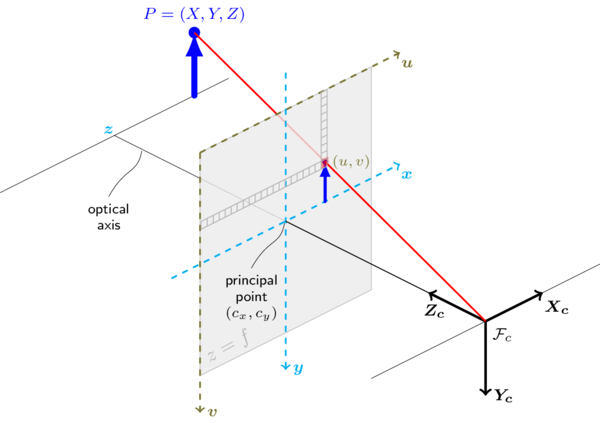
\includegraphics[width=0.6\textwidth]{chapter03/img/pinhole_camera_model.png}
    \caption[Pinhole Camera Model]{The pinhole camera model performs the perspective projection of three dimensional points into the plane. Real cameras additionally have a lense system that can result in radial and tangential distortion. These effects must be componsenated with a proper calibration of distortion models. The camera-coordinate-to-pixel-coordinate projection looses information on the depth. Therefore, the back projection results only in the direction of the light ray. The depth sensor gives the additional distance information to recover the point in camera coordinates. Graphic adopted from\cite{opencv_pinhole}.}\label{fig:pinhole_model}
\end{figure}
Figure~\ref{fig:pinhole_model} shows the perspective projection of three-dimensional points onto the plane.
This projection reduces the input dimension by one and is not depth preserving.

The model is parameterized by the focal length $f_x$ and $f_y$ that correspond to the distance of the pinhole to the image plane, the skew $s$ that resembles non-quadratic pixel shape and is most of the time $s = 0$ and the image center $c_x$ and $c_y$.

\subsubsection*{Forward Projection}

Let $\vec{P} = \rowvecxxx{X}{Y}{Z}$ be a world point in camera coordinates.
The perspective projection
\begin{equation}
    \vec{\hat{p}} = \colvecxxx{x}{y}{1} = \frac{1}{Z}\colvecxxx{X}{Y}{Z}
    \label{eq:pinhole_forward}
\end{equation}
results in the point $\vec{P}$ in image coordinates $\vec{\hat{p}}$. This step looses the depth information.
The image coordinates could be distorted and any correction would happen at this stage.
Multiplication of the $3 \times 3$ camera matrix $K$ and the homogeneous image coordinates results in the final pixel coordinates.
\begin{equation}
\begin{aligned}
K &= \begin{pmatrix}
        f_x & f_x s & c_x \\
        0   & f_y   & c_y \\
        0   & 0     & 1
     \end{pmatrix} \\
K \vec{\hat{p}} &= \begin{pmatrix}
        f_x & f_x s & c_x \\
        0   & f_y   & c_y \\
        0   & 0     & 1
     \end{pmatrix}\colvecxxx{x}{y}{1} = \colvecxxx{u}{v}{1} = \vec{p}
\end{aligned}
\end{equation}

\subsubsection*{Backward Projection}

Applying the inverse transformations allows to recover the direction of the light matching a pixel $\vec{p}$.
The potentially distorted image coordinates $\vec{\hat{p}}$ are obtained with the following formula.
\begin{equation}
\begin{aligned}
    \vec{\hat{p}} = \colvecxxx{x}{y}{1} &= K^{-1} \vec{p} \\
    \colvecxx{x}{y} &= \begin{pmatrix}\frac{1}{f_x} & -\frac{s}{f_y} \\ 0 & \frac{1}{f_y}\end{pmatrix} \colvecxx{u - c_x}{v - c_y}
\end{aligned}
\end{equation}
Again, if a distortion model is used, the inverse transformation needs to be applied to $\vec{\hat{p}}$.

The final step is the projection to the unit sphere that gives the direction vector of the light ray equivalent to norming the vector $\vec{\hat{p}}$.
\begin{equation}
    \colvecxxx{Xs}{Ys}{Zs} = \frac{1}{\sqrt{x^2 + y^2 + 1}} \colvecxxx{x}{y}{1}
    \label{eq:pinhole_backward}
\end{equation}

\subsubsection{Equirectangular Camera Model}

The equirectangular camera model maps the whole unit sphere to the plane.
Equirectangular images have constant, but potentially different angular resolution in $x$- and $y$-direction.
This mapping stores panoramas that are usually stitched together from multiple cameras.
The \acrshort{LIDAR} sensor output can be stored as an equirectangular image as well.
Supporting this camera model gives flexibility to support all kind of sensors as multiple pinhole sensors can be stitched to one virtual sensor and mapped to the equirectangular model.

\begin{figure}[H]
    \scalebox{0.9}{%
    

% Gradient Info
  
\tikzset {_5hbmo8yc4/.code = {\pgfsetadditionalshadetransform{ \pgftransformshift{\pgfpoint{81.84 bp } { -103.62 bp }  }  \pgftransformscale{1.32 }  }}}
\pgfdeclareradialshading{_42co7mn6x}{\pgfpoint{-72bp}{88bp}}{rgb(0bp)=(1,1,1);
rgb(0.052081516810825894bp)=(1,1,1);
rgb(25bp)=(0.74,0.74,0.74);
rgb(400bp)=(0.74,0.74,0.74)}
\tikzset{every picture/.style={line width=0.75pt}} %set default line width to 0.75pt        

\begin{tikzpicture}[x=0.75pt,y=0.75pt,yscale=-1,xscale=1,style = {font = \boldmath}]
%uncomment if require: \path (0,313); %set diagram left start at 0, and has height of 313

%Shape: Circle [id:dp5460928729364494] 
\draw  [draw opacity=0][shading=_42co7mn6x,_5hbmo8yc4][line width=1.5]  (24,163.5) .. controls (24,96.4) and (78.4,42) .. (145.5,42) .. controls (212.6,42) and (267,96.4) .. (267,163.5) .. controls (267,230.6) and (212.6,285) .. (145.5,285) .. controls (78.4,285) and (24,230.6) .. (24,163.5) -- cycle ;
%Straight Lines [id:da5671603358142259] 
\draw [color={rgb, 255:red, 74; green, 74; blue, 74 }  ,draw opacity=1 ] [dash pattern={on 4.5pt off 4.5pt}]  (145.5,163.5) -- (202,187.33) ;
%Shape: Ellipse [id:dp6506733150555541] 
\draw  [color={rgb, 255:red, 74; green, 74; blue, 74 }  ,draw opacity=1 ][dash pattern={on 4.5pt off 4.5pt}] (76,163.5) .. controls (76,96.4) and (107.12,42) .. (145.5,42) .. controls (183.88,42) and (215,96.4) .. (215,163.5) .. controls (215,230.6) and (183.88,285) .. (145.5,285) .. controls (107.12,285) and (76,230.6) .. (76,163.5) -- cycle ;
%Shape: Ellipse [id:dp26678317589757317] 
\draw  [color={rgb, 255:red, 74; green, 74; blue, 74 }  ,draw opacity=1 ][dash pattern={on 4.5pt off 4.5pt}][line width=0.75]  (24,163.5) .. controls (24,143.62) and (78.4,127.5) .. (145.5,127.5) .. controls (212.6,127.5) and (267,143.62) .. (267,163.5) .. controls (267,183.38) and (212.6,199.5) .. (145.5,199.5) .. controls (78.4,199.5) and (24,183.38) .. (24,163.5) -- cycle ;
%Straight Lines [id:da95744507209868] 
\draw [line width=2.25]    (145.5,163.5) -- (305.8,163.5) ;
\draw [shift={(310.8,163.5)}, rotate = 180] [fill={rgb, 255:red, 0; green, 0; blue, 0 }  ][line width=0.08]  [draw opacity=0] (14.29,-6.86) -- (0,0) -- (14.29,6.86) -- cycle    ;
%Straight Lines [id:da9220607301798066] 
\draw [color={rgb, 255:red, 74; green, 74; blue, 74 }  ,draw opacity=1 ] [dash pattern={on 4.5pt off 4.5pt}]  (202,91) -- (202,187.33) ;
%Shape: Arc [id:dp11613747224217108] 
\draw  [draw opacity=0][line width=1.5]  (179.38,177.98) .. controls (175.34,183.79) and (164.25,188) .. (151.5,188) .. controls (141.03,188) and (132.07,185.16) .. (127.41,180.92) -- (152.5,173.67) -- cycle ; \draw  [color={rgb, 255:red, 144; green, 19; blue, 254 }  ,draw opacity=1 ][line width=1.5]  (179.38,177.98) .. controls (175.34,183.79) and (164.25,188) .. (151.5,188) .. controls (141.03,188) and (132.07,185.16) .. (127.41,180.92) ;
%Shape: Arc [id:dp1998195952216596] 
\draw  [draw opacity=0][line width=1.5]  (166.45,136.09) .. controls (175.38,141.4) and (181.85,150.81) .. (182.82,161.52) .. controls (183.36,167.6) and (182.07,173.26) .. (179.38,177.98) -- (152.82,161.52) -- cycle ; \draw  [color={rgb, 255:red, 245; green, 166; blue, 35 }  ,draw opacity=1 ][line width=1.5]  (166.45,136.09) .. controls (175.38,141.4) and (181.85,150.81) .. (182.82,161.52) .. controls (183.36,167.6) and (182.07,173.26) .. (179.38,177.98) ;
%Straight Lines [id:da3798410950733011] 
\draw [color={rgb, 255:red, 65; green, 117; blue, 5 }  ,draw opacity=1 ][line width=1.5]    (145.5,163.5) -- (199.07,93.67) ;
\draw [shift={(201.5,90.5)}, rotate = 487.49] [fill={rgb, 255:red, 65; green, 117; blue, 5 }  ,fill opacity=1 ][line width=0.08]  [draw opacity=0] (11.61,-5.58) -- (0,0) -- (11.61,5.58) -- cycle    ;
%Shape: Circle [id:dp5016585286703897] 
\draw  [draw opacity=0][fill={rgb, 255:red, 74; green, 144; blue, 226 }  ,fill opacity=1 ] (198,91) .. controls (198,88.79) and (199.79,87) .. (202,87) .. controls (204.21,87) and (206,88.79) .. (206,91) .. controls (206,93.21) and (204.21,95) .. (202,95) .. controls (199.79,95) and (198,93.21) .. (198,91) -- cycle ;
%Straight Lines [id:da5083339397538952] 
\draw [line width=2.25]    (145.5,163.5) -- (96.54,212.46) ;
\draw [shift={(93,216)}, rotate = 315] [fill={rgb, 255:red, 0; green, 0; blue, 0 }  ][line width=0.08]  [draw opacity=0] (14.29,-6.86) -- (0,0) -- (14.29,6.86) -- cycle    ;
%Straight Lines [id:da9550893076013829] 
\draw [line width=2.25]    (145.5,163.5) -- (145.5,9.47) ;
\draw [shift={(145.5,4.47)}, rotate = 450] [fill={rgb, 255:red, 0; green, 0; blue, 0 }  ][line width=0.08]  [draw opacity=0] (14.29,-6.86) -- (0,0) -- (14.29,6.86) -- cycle    ;
%Shape: Circle [id:dp9507399492507013] 
\draw  [line width=1.5]  (24,163.5) .. controls (24,96.4) and (78.4,42) .. (145.5,42) .. controls (212.6,42) and (267,96.4) .. (267,163.5) .. controls (267,230.6) and (212.6,285) .. (145.5,285) .. controls (78.4,285) and (24,230.6) .. (24,163.5) -- cycle ;

% Text Node
\draw (168,107) node [anchor=north west][inner sep=0.75pt]  [color={rgb, 255:red, 65; green, 117; blue, 5 }  ,opacity=1 ] [align=left] {$\displaystyle \mathbf{r}$};
% Text Node
\draw (156.29,184.75) node [anchor=south east] [inner sep=0.75pt]  [color={rgb, 255:red, 144; green, 19; blue, 254 }  ,opacity=1 ] [align=left] {$\displaystyle \mathbf{\varphi }$};
% Text Node
\draw (160.5,145.5) node [anchor=north west][inner sep=0.75pt]  [color={rgb, 255:red, 245; green, 166; blue, 35 }  ,opacity=1 ] [align=left] {$\displaystyle \mathbf{\theta }$};


\end{tikzpicture}

    }
    \caption[Spherical Camera Model and Equirectangular Images]{Each cartesian point that is not the origin can be uniquely converted to spherical coordinates. The origin $\mathbf{O}$ is interpreted as an invalid measurement in the context of this thesis and therefore filtered out during processing.}\label{fig:spherical}
\end{figure}

The projections are mostly a conversion from cartesian to spherical coordinates and described here in brief.
Additionally, to suite the \acrshort{LIDAR} sensor better a slight addition for a vertical field of view is added.
This field of view simply crops the full equirectangular image to the predefined slice and discards other coordinates as invalid.
Figure~\ref{fig:spherical} shows the relationship between points in spherical coordinates and the equirectangular projection.

The model is parametrized by the width $w$ and height $h$ of the image and the vertical field of view $[\theta_{min}, \theta_{max}]$ which defaults to $\theta_{min} = 0$ and $\theta_{max} = \pi$.
This definition yields the vertical and horizontal angular resolution of a pixel, which is a constant.
\begin{equation}
\label{eq:equi_angular_resolution}
\begin{aligned}
    d\varphi &= \frac{2 \pi}{w} \\
    d\theta &= \frac{\theta_{max} - \theta_{min}}{h} \\
\end{aligned}
\end{equation}
The used spherical coordinates $z = (r, \varphi, \theta)$ convention defines the radius $r \in \mathbb{R}$, the azimuthal angle $\varphi \in [-\pi, \pi)$ and the polar angle $\theta \in [0, \pi]$.
Measurements with $r = 0$ are filtered out as invalid data points.

\subsubsection*{Forward Projection}

Let $\vec{P} = \rowvecxxx{X}{Y}{Z}$ be a point in camera coordinates.
This point is converted to spherical coordinates.
\begin{equation}
\begin{aligned}
    r       &= \sqrt{X^2 + Y^2 + Z^2} \\
    \theta  &= \arccos{\frac{Z}{r}} \\
    \varphi &= \arctantwo{\frac{Y}{X}}
\end{aligned}
\end{equation}
This conversion is ill defined for $r = 0$ which corresponds to a missing range measurement and can be skipped safely.
Finally, the spherical coordinates are converted to pixel coordinates with
\begin{equation}
\begin{aligned} 
    \colvecxx{u}{v} = \colvecxx{\frac{\varphi + \pi}{d\varphi}}{\frac{\theta}{d\theta}}
\end{aligned}
\end{equation}

\subsubsection*{Backward Projection}

The backward projection recovers the light ray direction from pixel coordinates.
It is analogous to the forward projection mainly a conversion from spherical to cartesian coordinates.
Note, that $r = 1$ as the resulting vector is of unit length.
\begin{equation}
\begin{aligned}
    \varphi &= u d\varphi - \pi \\
    \theta &= \theta_{min} + v d\theta \\
    \colvecxxx{X_s}{Y_s}{Z_s} &= \colvecxxx{\sin \theta \cos \varphi}{\sin \theta \sin \varphi}{\cos \theta}
\end{aligned}
\end{equation}

\subsubsection{Range and Depth Conversion}\label{sec:range_depth_conversion}

\begin{figure}[H]
    \scalebox{0.8}{%
    

\tikzset{every picture/.style={line width=0.75pt}} %set default line width to 0.75pt        

\begin{tikzpicture}[x=0.75pt,y=0.75pt,yscale=-1,xscale=1]
%uncomment if require: \path (0,273); %set diagram left start at 0, and has height of 273

%Straight Lines [id:da7423207506186664] 
\draw [line width=3.75]    (17.08,234.29) -- (243.08,234.29) ;
%Straight Lines [id:da2664879119929795] 
\draw    (50.5,40.5) -- (50.5,234.92) ;
%Straight Lines [id:da2932541940464021] 
\draw [color={rgb, 255:red, 208; green, 2; blue, 27 }  ,draw opacity=1 ]   (50.5,40.5) -- (176.08,234.29) ;
%Shape: Circle [id:dp5274939901831479] 
\draw  [draw opacity=0][fill={rgb, 255:red, 0; green, 0; blue, 0 }  ,fill opacity=1 ] (170.02,234.29) .. controls (170.02,230.94) and (172.74,228.23) .. (176.08,228.23) .. controls (179.43,228.23) and (182.15,230.94) .. (182.15,234.29) .. controls (182.15,237.64) and (179.43,240.35) .. (176.08,240.35) .. controls (172.74,240.35) and (170.02,237.64) .. (170.02,234.29) -- cycle ;
%Shape: Circle [id:dp5178837685841811] 
\draw  [draw opacity=0][fill={rgb, 255:red, 0; green, 0; blue, 0 }  ,fill opacity=1 ] (44.44,40.5) .. controls (44.44,37.15) and (47.15,34.44) .. (50.5,34.44) .. controls (53.85,34.44) and (56.56,37.15) .. (56.56,40.5) .. controls (56.56,43.85) and (53.85,46.56) .. (50.5,46.56) .. controls (47.15,46.56) and (44.44,43.85) .. (44.44,40.5) -- cycle ;

% Text Node
\draw (114.53,100) node [anchor=north west][inner sep=0.75pt]  [color={rgb, 255:red, 208; green, 2; blue, 27 }  ,opacity=1 ,rotate=-56.88] [align=left] {range $\displaystyle r$};
% Text Node
\draw (71,73) node [anchor=north west][inner sep=0.75pt]  [rotate=-90] [align=left] {orthographic depth $\displaystyle d$};
% Text Node
\draw (110,246) node [anchor=north west][inner sep=0.75pt]  [color={rgb, 255:red, 0; green, 0; blue, 0 }  ,opacity=1 ] [align=left] {camera center $\displaystyle \mathbf{C}$};
% Text Node
\draw (46,6) node [anchor=north west][inner sep=0.75pt]   [align=left] {$\displaystyle \mathbf{P}$};


\end{tikzpicture}


    }
    \caption[Orthographic Depth and Range visualized]{The distance information of a point relative to the center of a sensor at $\vec{C}$ can either be stored as the orthographic depth, mathematically the $Z$ component of the camera coordinates or the range, equivalent to the $L2$ norm of the point $\vec{P}$ in camera coordinates. The orthographic depth is commonly provided by depth cameras and the range by \acrshort{LIDAR} systems.}
    \label{fig:range_depth}
\end{figure}

There are two possible conventions on how to store depth data, both demonstrated in figure~\ref{fig:range_depth}.
The orthographic depth $d$ is the distance from the image plane and commonly returned by pinhole depth sensors like the Kinectv2.
On the other hand, the range $r$ is the $L2$ norm of the vector from the camera origin to $\vec{P}$.
For consistency and generality, depth data is converted to range data before further processing takes place.
This simplifies later conversion and mixing of different camera models in a coherent fashion.
The conversion depends on the camera model and only the pinhole model is subject to analysis here.

From the forward projection function~\ref{eq:pinhole_forward} of the pinhole model follows the connection of the range and orthographic depth of the camera coordinates $\vec{P}$ and image coordinates $\vec{\hat{p}}$ of the point $\mathbf{P}$.
\begin{equation}
\begin{aligned}
    &\vec{\hat{p}} = \colvecxxx{x}{y}{1} = \frac{1}{Z}\colvecxxx{X}{Y}{Z} \\
    \implies &Z \vec{\hat{p}} = \vec{P} \\
    \implies &Z \lnorm{\vec{\hat{p}}} = \lnorm{\vec{P}}
\end{aligned}
\end{equation}
The inverse of the $Z_{s}$ component of the backward projection from equation~\ref{eq:pinhole_backward} provides the scaling factor between orthographic depth and range.
Consequently, the range $r$ for the depth $d$ at image coordiantes $\rowvecxx{x}{y}$ with corresponding coordinates on the unit sphere $\rowvecxxx{X_s}{Y_s}{Z_s}$ is computed with
\begin{equation}
    r = \frac{d}{Z_s} = d \sqrt{x^2 + y^2 + 1}\text{.}
\end{equation}

\subsection{Keypoint Detection and Feature Description}

Extracting information from images is a common task in computer vision.
One approach is the detection of salient regions of special interest --- \emph{features}.
Such regions can have arbitrary detectable properties, like a sharp brightness gradient or being corner-like.
Detecting such a region results in a \emph{keypoint} that might have properties like a \emph{size}, \emph{response} and sometimes even an \emph{orientation} (Figure~\ref{fig:features_example}).
\begin{figure}[H]
    \scalebox{0.95}{%
    

\tikzset{every picture/.style={line width=0.75pt}} %set default line width to 0.75pt        

\begin{tikzpicture}[x=0.75pt,y=0.75pt,yscale=-1,xscale=1]
%uncomment if require: \path (0,241); %set diagram left start at 0, and has height of 241

%Shape: Rectangle [id:dp035829742459278835] 
\draw   (10,9.33) -- (283,9.33) -- (283,207.33) -- (10,207.33) -- cycle ;
%Shape: Polygon [id:ds9920063897845183] 
\draw  [fill={rgb, 255:red, 0; green, 0; blue, 0 }  ,fill opacity=1 ] (134,82.33) -- (178,135.33) -- (116,112.33) -- (60,129.33) -- (56,85.33) -- cycle ;
%Shape: Circle [id:dp761043588130765] 
\draw  [draw opacity=0][fill={rgb, 255:red, 74; green, 144; blue, 226 }  ,fill opacity=1 ] (173,135.33) .. controls (173,132.57) and (175.24,130.33) .. (178,130.33) .. controls (180.76,130.33) and (183,132.57) .. (183,135.33) .. controls (183,138.09) and (180.76,140.33) .. (178,140.33) .. controls (175.24,140.33) and (173,138.09) .. (173,135.33) -- cycle ;
%Shape: Circle [id:dp13055646965010093] 
\draw  [draw opacity=0][fill={rgb, 255:red, 74; green, 144; blue, 226 }  ,fill opacity=1 ] (129,82.33) .. controls (129,79.57) and (131.24,77.33) .. (134,77.33) .. controls (136.76,77.33) and (139,79.57) .. (139,82.33) .. controls (139,85.09) and (136.76,87.33) .. (134,87.33) .. controls (131.24,87.33) and (129,85.09) .. (129,82.33) -- cycle ;
%Shape: Circle [id:dp8680057373610014] 
\draw  [draw opacity=0][fill={rgb, 255:red, 74; green, 144; blue, 226 }  ,fill opacity=1 ] (111,112.33) .. controls (111,109.57) and (113.24,107.33) .. (116,107.33) .. controls (118.76,107.33) and (121,109.57) .. (121,112.33) .. controls (121,115.09) and (118.76,117.33) .. (116,117.33) .. controls (113.24,117.33) and (111,115.09) .. (111,112.33) -- cycle ;
%Shape: Circle [id:dp7411102135218419] 
\draw  [draw opacity=0][fill={rgb, 255:red, 74; green, 144; blue, 226 }  ,fill opacity=1 ] (55,129.33) .. controls (55,126.57) and (57.24,124.33) .. (60,124.33) .. controls (62.76,124.33) and (65,126.57) .. (65,129.33) .. controls (65,132.09) and (62.76,134.33) .. (60,134.33) .. controls (57.24,134.33) and (55,132.09) .. (55,129.33) -- cycle ;
%Shape: Circle [id:dp2075524582431375] 
\draw  [draw opacity=0][fill={rgb, 255:red, 74; green, 144; blue, 226 }  ,fill opacity=1 ] (51,85.33) .. controls (51,82.57) and (53.24,80.33) .. (56,80.33) .. controls (58.76,80.33) and (61,82.57) .. (61,85.33) .. controls (61,88.09) and (58.76,90.33) .. (56,90.33) .. controls (53.24,90.33) and (51,88.09) .. (51,85.33) -- cycle ;
%Shape: Polygon [id:ds2941998606572992] 
\draw  [fill={rgb, 255:red, 0; green, 0; blue, 0 }  ,fill opacity=1 ] (463,82.33) -- (507,135.33) -- (449,107.33) -- (415,118.33) -- (413,89.33) -- cycle ;
%Shape: Circle [id:dp23309094023669752] 
\draw  [draw opacity=0][fill={rgb, 255:red, 245; green, 166; blue, 35 }  ,fill opacity=1 ] (502,135.33) .. controls (502,132.57) and (504.24,130.33) .. (507,130.33) .. controls (509.76,130.33) and (512,132.57) .. (512,135.33) .. controls (512,138.09) and (509.76,140.33) .. (507,140.33) .. controls (504.24,140.33) and (502,138.09) .. (502,135.33) -- cycle ;
%Shape: Circle [id:dp6238978047230974] 
\draw  [draw opacity=0][fill={rgb, 255:red, 245; green, 166; blue, 35 }  ,fill opacity=1 ] (458,82.33) .. controls (458,79.57) and (460.24,77.33) .. (463,77.33) .. controls (465.76,77.33) and (468,79.57) .. (468,82.33) .. controls (468,85.09) and (465.76,87.33) .. (463,87.33) .. controls (460.24,87.33) and (458,85.09) .. (458,82.33) -- cycle ;
%Shape: Circle [id:dp6090832055278774] 
\draw  [draw opacity=0][fill={rgb, 255:red, 245; green, 166; blue, 35 }  ,fill opacity=1 ] (444,107.33) .. controls (444,104.57) and (446.24,102.33) .. (449,102.33) .. controls (451.76,102.33) and (454,104.57) .. (454,107.33) .. controls (454,110.09) and (451.76,112.33) .. (449,112.33) .. controls (446.24,112.33) and (444,110.09) .. (444,107.33) -- cycle ;
%Shape: Circle [id:dp846464460393933] 
\draw  [draw opacity=0][fill={rgb, 255:red, 245; green, 166; blue, 35 }  ,fill opacity=1 ] (410,118.33) .. controls (410,115.57) and (412.24,113.33) .. (415,113.33) .. controls (417.76,113.33) and (420,115.57) .. (420,118.33) .. controls (420,121.09) and (417.76,123.33) .. (415,123.33) .. controls (412.24,123.33) and (410,121.09) .. (410,118.33) -- cycle ;
%Shape: Circle [id:dp4845841454073171] 
\draw  [draw opacity=0][fill={rgb, 255:red, 245; green, 166; blue, 35 }  ,fill opacity=1 ] (408,89.33) .. controls (408,86.57) and (410.24,84.33) .. (413,84.33) .. controls (415.76,84.33) and (418,86.57) .. (418,89.33) .. controls (418,92.09) and (415.76,94.33) .. (413,94.33) .. controls (410.24,94.33) and (408,92.09) .. (408,89.33) -- cycle ;
%Shape: Polygon [id:ds0993695896079676] 
\draw   (340,43.33) -- (612,9.33) -- (612,206.33) -- (340,182.33) -- cycle ;
%Shape: Square [id:dp8236130174233348] 
\draw  [color={rgb, 255:red, 208; green, 2; blue, 27 }  ,draw opacity=1 ][dash pattern={on 4.5pt off 4.5pt}] (153,110.33) -- (203,110.33) -- (203,160.33) -- (153,160.33) -- cycle ;
%Shape: Square [id:dp6761472971368142] 
\draw  [color={rgb, 255:red, 208; green, 2; blue, 27 }  ,draw opacity=1 ][dash pattern={on 4.5pt off 4.5pt}] (109,57.33) -- (159,57.33) -- (159,107.33) -- (109,107.33) -- cycle ;
%Shape: Square [id:dp06523745964376726] 
\draw  [color={rgb, 255:red, 208; green, 2; blue, 27 }  ,draw opacity=1 ][dash pattern={on 4.5pt off 4.5pt}] (31,60.33) -- (81,60.33) -- (81,110.33) -- (31,110.33) -- cycle ;
%Shape: Square [id:dp3887475640832124] 
\draw  [color={rgb, 255:red, 208; green, 2; blue, 27 }  ,draw opacity=1 ][dash pattern={on 4.5pt off 4.5pt}] (91,87.33) -- (141,87.33) -- (141,137.33) -- (91,137.33) -- cycle ;
%Shape: Square [id:dp6775183704136505] 
\draw  [color={rgb, 255:red, 208; green, 2; blue, 27 }  ,draw opacity=1 ][dash pattern={on 4.5pt off 4.5pt}] (35,104.33) -- (85,104.33) -- (85,154.33) -- (35,154.33) -- cycle ;
%Shape: Square [id:dp0686549638078735] 
\draw  [color={rgb, 255:red, 208; green, 2; blue, 27 }  ,draw opacity=1 ][dash pattern={on 4.5pt off 4.5pt}] (388,64.33) -- (438,64.33) -- (438,114.33) -- (388,114.33) -- cycle ;
%Shape: Square [id:dp20553871041489524] 
\draw  [color={rgb, 255:red, 208; green, 2; blue, 27 }  ,draw opacity=1 ][dash pattern={on 4.5pt off 4.5pt}] (438,57.33) -- (488,57.33) -- (488,107.33) -- (438,107.33) -- cycle ;
%Shape: Square [id:dp9372102954632048] 
\draw  [color={rgb, 255:red, 208; green, 2; blue, 27 }  ,draw opacity=1 ][dash pattern={on 4.5pt off 4.5pt}] (482,110.33) -- (532,110.33) -- (532,160.33) -- (482,160.33) -- cycle ;
%Shape: Square [id:dp5089024455920732] 
\draw  [color={rgb, 255:red, 208; green, 2; blue, 27 }  ,draw opacity=1 ][dash pattern={on 4.5pt off 4.5pt}] (390,93.33) -- (440,93.33) -- (440,143.33) -- (390,143.33) -- cycle ;
%Shape: Square [id:dp7886399279303968] 
\draw  [color={rgb, 255:red, 208; green, 2; blue, 27 }  ,draw opacity=1 ][dash pattern={on 4.5pt off 4.5pt}] (424,82.33) -- (474,82.33) -- (474,132.33) -- (424,132.33) -- cycle ;

% Text Node
\draw (269,214) node [anchor=north west][inner sep=0.75pt]   [align=left] {$\displaystyle I_{1}$};
% Text Node
\draw (592,212) node [anchor=north west][inner sep=0.75pt]   [align=left] {$\displaystyle I_{2}$};
% Text Node
\draw (44,136.33) node [anchor=north west][inner sep=0.75pt]   [align=left] {$\displaystyle  \begin{array}{{>{\displaystyle}l}}
\mathbf{K}_{1,1}\\
\end{array}$};
% Text Node
\draw (145,73.33) node [anchor=north west][inner sep=0.75pt]   [align=left] {$\displaystyle  \begin{array}{{>{\displaystyle}l}}
\mathbf{K}_{1,2}\\
\end{array}$};
% Text Node
\draw (27,60.33) node [anchor=north west][inner sep=0.75pt]   [align=left] {$\displaystyle  \begin{array}{{>{\displaystyle}l}}
\mathbf{K}_{1,3}\\
\end{array}$};
% Text Node
\draw (180,138.33) node [anchor=north west][inner sep=0.75pt]  [color={rgb, 255:red, 155; green, 155; blue, 155 }  ,opacity=1 ] [align=left] {$\displaystyle  \begin{array}{{>{\displaystyle}l}}
\mathbf{K}_{1,4}\\
\end{array}$};
% Text Node
\draw (102,121.33) node [anchor=north west][inner sep=0.75pt]   [align=left] {$\displaystyle  \begin{array}{{>{\displaystyle}l}}
\mathbf{K}_{1,5}\\
\end{array}$};
% Text Node
\draw (391,127.33) node [anchor=north west][inner sep=0.75pt]   [align=left] {$\displaystyle  \begin{array}{{>{\displaystyle}l}}
\mathbf{K}_{2,4}\\
\end{array}$};
% Text Node
\draw (473,56.33) node [anchor=north west][inner sep=0.75pt]   [align=left] {$\displaystyle  \begin{array}{{>{\displaystyle}l}}
\mathbf{K}_{2,2}\\
\end{array}$};
% Text Node
\draw (434,115.83) node [anchor=north west][inner sep=0.75pt]   [align=left] {$\displaystyle  \begin{array}{{>{\displaystyle}l}}
\mathbf{K}_{2,3}\\
\end{array}$};
% Text Node
\draw (374,68.33) node [anchor=north west][inner sep=0.75pt]   [align=left] {$\displaystyle  \begin{array}{{>{\displaystyle}l}}
\mathbf{K}_{2,1}\\
\end{array}$};
% Text Node
\draw (509,138.33) node [anchor=north west][inner sep=0.75pt]   [align=left] {$\displaystyle  \begin{array}{{>{\displaystyle}l}}
\mathbf{K}_{2,5}\\
\end{array}$};


\end{tikzpicture}


    }
    \caption[Schematic feature detection and matching]{\emph{Schematic feature detection and matching.} This figure displays two polygons from different view points. The feature detection algorithm detects the corners of the polygon as keypoints in both images. The order of detection is not stable and establishing the correspondence between the detected keypoints requires further processing. A feature descriptor examines to local neighbourhood of each keypoint, visualized with the red dotted square. This descriptor is then used to find the most similar region around a keypoint of the other image. This process is called \emph{feature matching}.}\label{fig:features_example}
\end{figure}
Keypoints on itself are not descriptive enough to be identified in different images.
A changing view point or even a different camera result in changes to the overall shape and appearance of the scene.
Reliable keypoint identification requires the analysis of bigger image patches.
The \emph{keypoint descriptor} analyzes a predefined region around the centered keypoint and extracts a vector for that region.
Different aspects can be analyzed and Section~\ref{sec:feature_algorithms} introduces the most common algorithms for that task.
The extracted vector has a high dimension with tens to hundreds of elements.

Connecting the keypoints between different images uses the extracted descriptors for each keypoint.
\emph{Similar} descriptors are associated.
Similarity of the descriptors is calculated with a matching norm depdendent on the structure of the descriptor.
Dense real descriptors commonly use the Euclidean norm where as binary descriptors use the hamming norm.
Additional constraints, like geometric consistency, improve the accuracy of the matching result.
For the provided example this result might be
\begin{equation}
\begin{aligned}
    \mathbf{K_{1,2}} &\leftrightarrow \mathbf{K_{2,2}}~\textcolor{darkgreen}{\bullet} &
    \mathbf{K_{1,4}} &\leftrightarrow \mathbf{K_{2,5}}~\textcolor{darkgreen}{\bullet} &
    \mathbf{K_{1,5}} &\leftrightarrow \mathbf{K_{2,3}}~\textcolor{darkgreen}{\bullet} \\
    \mathbf{K_{1,3}} &\leftrightarrow \mathbf{K_{2,4}} &
    \mathbf{K_{1,1}} &\leftrightarrow \mathbf{K_{2,1}} &
\end{aligned}
\end{equation}
with green bullets indicating a correct match.
An important descriptor design criteria is the trade-off between computational cost and descriptive power, as especially descriptor matching is computationally expensive.

Features play a key role in multiple computer vision tasks.
Place or object recognition and document searching rely on the identification of similar descriptors in queried image to already indexed descriptors of known images.
Typically, storage and computational constrains require preprocessing the descriptors with clustering techniques to reduce the number of descriptors to store and allow hierarchical matching.

The second major application is visual odometry and \gls{sfm}.
Corresponding keypoints provide landmarks for triangulation and pose reconstruction.
The relative pose between the two camera is computed with Nistér's 5-point algorithm\cite{nister_ieee2004}.
To obtain a stable and consistent result for the pose the \acrshort{RANSAC} (\acrlong{RANSAC})\cite{fischler_ransac_1980} algorithm performs multiple pose computations with random subsets of keypoint correspondences.
The assumed pose is used to project the keypoints from one image into the other.
A high pixel distance for the projected keypoints to the expected keypoints indicates a wrong pose, showing that the used subset of keypoints for the pose calculation had false matches.
After multiple iterations, a consensus pose might be obtained and can be optimized as final pose.
If no such consensus pose exists, the image pair is rejected.

Establishing the correspondence between keypoints of multiple images can be supported by using additional heuristics for descriptor matching.
The first heuristic is \emph{cross checking}.
Descriptors correspond only if the distance of the descriptors is minimal in both directions.
The second commonly used heuristic is \emph{Lowe's ratio check}\cite{lowe_ijcv04} putting the best and second best descriptor match distance into relation and requiring a certain distance ratio to be superseded.
The last simple heuristic is the definition of an \emph{upper bound} for the match distance.
Improvements to \acrshort{RANSAC}\cite{sattler_iccv2009,chum_cvpr2005} use more sophisticated keypoint sampling criteria by exploiting spatial consistency or the descriptor distance.

More complicated keypoint preprocessing can be done to reduce the number of descriptors to match.
Keypoints can be discarded to achieve a higher spread over the image and avoid clusters of keypoints that provoke descriptor ambiguity.
The detector response is another important criteria for sorting keypoints by quality.
If apriori information of the approximate motion of the camera is known matches can be ranked based on the expected displacement of the keypoint.

\subsection{Statistics of Binary Classifiers}\label{sec:statistic_classifier}

Evaluating the performance of the feature matching algorithms on the converted depth images is done by analyzing the matching process as a binary classifier.
The classification task is to determine if a keypoint $\mathbf{K_1}$ of image $I_1$ corresponds with keypoint $\mathbf{K_2}$ in image $I_2$ with a binary outcome.
A pair of keypoints corresponds, if both pixel coordinates projected into space intersect at the same point, allowing for a little bit of uncertainty, e.g. 2\,px backprojection difference.
As with most statistics, it is necessary to consider the distribution of a quantity and analyze it from multiple view points.
Therefore, the final evaluation will consider other criteria, like distribution and characteristics of the keypoints.

Pairs of keypoints are defined as \emph{positive} ($P$) if they correspond and \emph{negative} ($N$) otherwise.
The predicted outcome of the matching system is either \emph{yes} ($y$) or \emph{no} ($n$).
The result of this prediction is in one of four categories.
A correspondence can be correctly, a \emph{true positive} ($TP$), or mistakenly recognized, a \emph{false positive} ($FP$).
Similarly, the lack of correspondence can be either correctly or incorrectly, so called \emph{true negatives} ($TN$) and \emph{false negatives} ($FN$), detected.
The \emph{confusion matrix}, a specialized case of a \emph{contingency table}\cite{agresti_2007}, keeps track of classification outcomes and is the basis for many performance criteria and derived metrics.
Table~\ref{tab:def_confusion_matrix} demonstrates the arrangement of elements in a confusion matrix.
The provided values can be either an absolute count of elements or a relative share of total elements and must be exhaustive.

{\renewcommand{\arraystretch}{1.2}%
\begin{table}[H]
\setlength\tabcolsep{0.5em}
\begin{tabular}{r|c|c|l}
    \multicolumn{1}{r}{} &
    \multicolumn{1}{c}{$P$} &
    \multicolumn{1}{c}{$N$} &
    \multicolumn{1}{l}{} \\
  \cline{2-3}
  $y$ & $TP$  & $FP$ & Total \emph{yes} \\
  \cline{2-3}
  $n$ & $FN$  & $TN$ & Total \emph{no} \\
  \cline{2-3}
    \multicolumn{1}{r}{} &
    \multicolumn{1}{c}{Total \emph{Positives} ($\#P$)} &
    \multicolumn{1}{c}{Total \emph{Negatives} ($\#N$)}
\end{tabular}
\caption[Definition of the confusion matrix]{\emph{Definition of the confusion matrix.} A confusion matrix summarizes the decision quality of a binary classifier. The elements to be classified can be in either category; \emph{positive} ($P$) or \emph{negative} ($N$). Correct classifications of elements are either \emph{true positives} ($TP$) or \emph{true negatives} ($TN$). Misclassification results in \emph{false positives} ($FP$) or \emph{false negatives} ($FN$).}\label{tab:def_confusion_matrix}
\end{table}}

All \emph{positive} elements are \emph{relevant elements} in the sense, that the keypoint pair points to the same world coordinate.
Predicted correspondences ($y$) are called \emph{selected elements}.
Different common ratios are derived from the confusion matrix.

\begin{description}
    \item[True Positive Rate] The true positive rate defines the ratio of correctly identified positive elements to total positive elements and is also called \textbf{hit rate}, \textbf{recall} or \textbf{sensitivity}.
        \begin{equation}
            TPR = \frac{TP}{\#P}
            \label{eq:true_positive_rate}
        \end{equation}
    \item[False Positive Rate] This ratio shows how many negative elements are mistakenly classified as positive elements. It is sometimes named \textbf{false alarm rate} or \textbf{fallout}.
        \begin{equation}
            FPR = \frac{FP}{\#N}
            \label{eq:false_positive_rate}
        \end{equation}
    \item[True Negative Rate] Also called \textbf{specificity}, the true negative rate is the ratio of correctly rejected elements.
        \begin{equation}
        \begin{aligned}
            TNR &= \frac{TN}{\#N} \\
                &= 1 - FPR
        \end{aligned}
        \label{eq:true_negative_rate}
        \end{equation}
    \item[Accuracy] The accuracy is the percentage of correctly classified elements. This measure is called \textbf{Rand index} in data clustering.
        \begin{equation}
            A = \frac{TP + TN}{\#P + \#N} = \frac{TP + TN}{TP + FP + TN + FN}
            \label{eq:accuracy}
        \end{equation}
    \item[Precision] The precision is the ratio of positive elements in all selected elements.
        \begin{equation}
            precision = \frac{TP}{TP + FP}
        \end{equation}
\end{description}
Each of these ratios can be of any value between $[0, 1]$ and might be written as a percentage.
Both precision and recall are commonly used to compare and evaluate feature matching algorithms and keypoint descriptors.
The proposed metric share the pitfall, that a low number of total elements or highly skewed data can result in very strong results for each metric, but correspond to a weak real world performance.

\subsubsection{Receiver Operating Statistics Analysis}

Choosing a suitable configuration or algorithm combination requires trade-offs between different aspects of the final system.
\acrlong{ROC} (\acrshort{ROC}) analysis\cite{fawcett_2006} provides a tool to visualize the trade-offs between different systems.
The central component of this analysis are the \emph{\acrshort{ROC} graphs}.
They plot the false positive rate and true positive rate, the \emph{\acrshort{ROC} space}, of multiple classifiers in one graph, with Figure~\ref{fig:roc_graph} containing all qualitatively different cases.
\begin{figure}[H]
\begin{tikzpicture}
\begin{axis}[xmin=0,xmax=1,ymin=0,ymax=1,samples=50,xlabel={false positive rate}, ylabel={true positive rate},grid=major]
  \addplot[gray, dashed] (x,x);
  \node[label={315:{$\mathbf{A}$}},circle,fill,inner sep=2pt] at (axis cs:0.01,0.99) {};
  \node[label={315:{$\mathbf{B}$}},circle,fill,inner sep=2pt] at (axis cs:0.2,0.2) {};
  \node[label={315:{$\mathbf{C}$}},circle,fill,inner sep=2pt] at (axis cs:0.2,0.5) {};
  \node[label={315:{$\mathbf{D}$}},circle,fill,inner sep=2pt] at (axis cs:0.35,0.65) {};
  \node[label={315:{$\mathbf{E}$}},circle,fill,inner sep=2pt] at (axis cs:0.4,0.3) {};
\end{axis}
\end{tikzpicture}
\caption[The elements of a \acrshort{ROC} graph]{\emph{The elements of a \acrshort{ROC} graph.} A \acrshort{ROC} graph plots the true positive rate versus the false positive rate of a binary classifier. Each point is one classification system. The diagonal $f(x) = x$ is equivalent to a 50\% chance of correct classification and a system on this line has no predictive power, as in this case $\mathbf{B}$. Points above this line ($\mathbf{A}$, $\mathbf{C}$, $\mathbf{D}$) indicate better-than-random performance and the bigger the distance to this diagonal the higher the informedness, also called Youden-Index, of this system. The optimal classifier ($\mathbf{A}$) is in the topleft corner and has no false decisions. Points below the diagonal ($\mathbf{E}$) might still have predictive power but indicate a wrong labeling of the outcomes.}\label{fig:roc_graph}
\end{figure}

Points above the diagonal have predictive power proportional to the distance to the diagonal.
This distance is also called the \textbf{Youden-Index} $\mathbf{J}$\cite{youden_cancer1950} and is a measure of informedness of the classifier:
\begin{equation}
\begin{aligned}
    J &= sensitivity + specificity - 1
      &= \frac{TP}{TP + FN} + \frac{TN}{TN + FP} - 1\text{.}
\end{aligned}
\label{eq:youden}
\end{equation}
Unless there are no samples tested, the Youden-Index is $\mathbf{J} \in [0, 1]$.
The higher $\mathbf{J}$ the better the two groups are separated by the classifier.
\acrshort{ROC} analysis gives a valueable instrument to compare the relative performance of classifiers.
A final judgement requires to take additional measures like absolute number of classified elements into account.
Fawcett's\cite{fawcett_2006} work provides a more detailed introduction to \acrshort{ROC} analysis in machine learning.

\newpage

\section{Depth Image Processing}

Depth images are disturbed by different error sources and intrinsic noise of the sensory system.
Common issues are reflections from water or glass, transparent objects and infrared light sources.
Objects outside the range of the sensor or otherwise incorrect measurements result in a $0$ in the depth image.
The continuous measurements are stored as depth images in conventional lossless image formats like png.
This requires to quantize the distance values to integers.
Effects of these conditions can be partially mitigated by preprocessing and filtering.

\subsection{Edge-Preserving Filtering}

Filtering is an operation to reduce the impact of sensor noise from limited resolution and other random effects on measured quantities.
These deviations propagate through the feature image conversion.
The feature images, introduced in Section~\ref{sec:feature_images}, build upon information information about changes in the geometry of sensed objects.
Therefore, sharp changes, e.g.~edges and corners, shall be preserved by the filter, requiring edge-preserving filters.
Each tested filter uses OpenCV's\cite{opencv_library} proven and readily available implementations.

\subsubsection{Median Blur}

Median Blur, introduced to image processing by Frieden\cite{frieden_new76}, is a well established technique to reduce salt-and-pepper noise and is an effective edge-preserving filter.
The filter modifies each pixel of the image equally.
A window of $n \times m$ pixels with $n,m \in \mathbb{N}_{2k + 1}$ is centered at the pixel.
The median of all pixels in that window is calculated and stored as the new value.
Floating point operations are not required and the filter is implementable with $\mathcal{O}(n)$\cite{huang_ieee79} time complexity.
$n$ and $m$ are the controllable parameters.
OpenCV's\cite{opencv_library} implementation additionally utilizes \acrshort{SIMD} instructions for increased processing speed.

\subsubsection{Bilateral Filter}

Bilateral filtering, introduced by Tomasi and Manduchi\cite{tomasi_iccv98}, considers two factors in the filtering process.
\emph{Spatial closeness}, similar to median filtering, and \emph{similarity} of the values are combined in the bilateral filter.
Its application is convolutional, similar to the median blur and other filters.
Each neighbouring pixel's effect on the central pixel is weighted by a geometric \emph{closeness} and \emph{similarity} function.
Similarity can be based on a classical distance norm of photometric values, like brightness, or be more sophisticated, like perceived similarity.
A common function for both aspects is a Gaussian kernel with the Euclidean norm as distance measure.
Figure~\ref{fig:bilateral_filter} provides an example application of the bilateral filter on a single channel, two-dimensional signal with the Gaussian function for \emph{closeness} and \emph{similarity}.
\begin{figure}[H]
    \begin{subfigure}[b]{0.3\linewidth}
        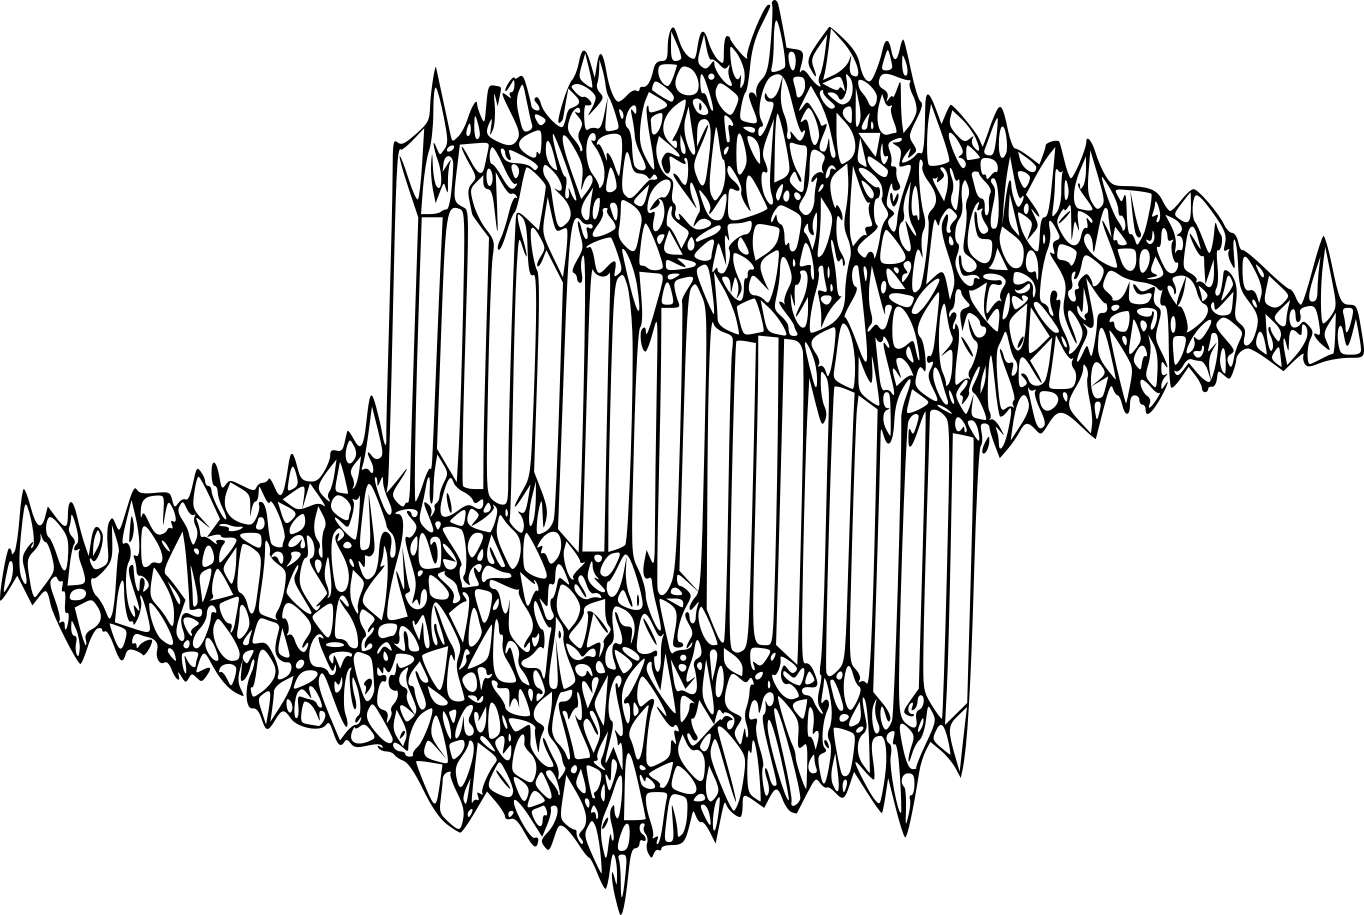
\includegraphics[width=\linewidth]{chapter04/img/bilateral1.png}
        \caption{}\label{fig:bilateral_1}
    \end{subfigure}
    \begin{subfigure}[b]{0.3\linewidth}
        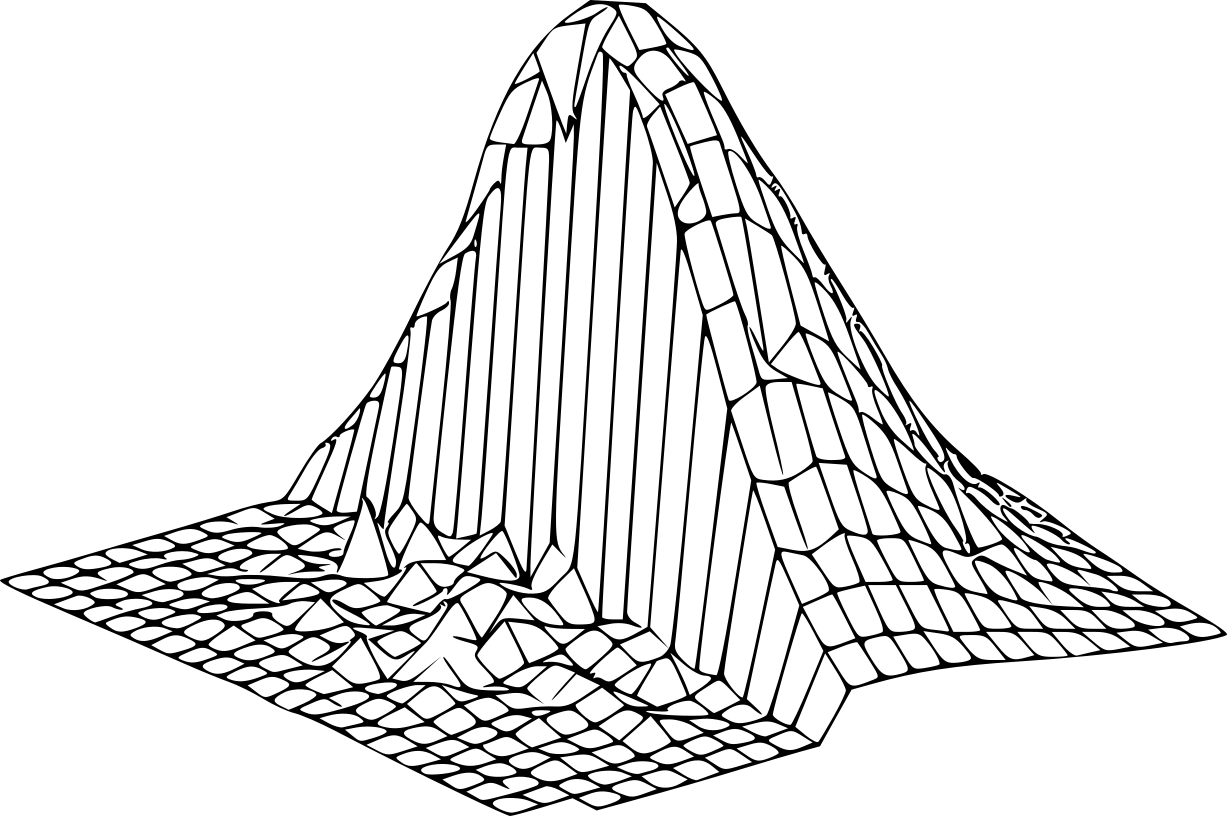
\includegraphics[width=\linewidth]{chapter04/img/bilateral2.png}
        \caption{}\label{fig:bilateral_2}
    \end{subfigure}
    \begin{subfigure}[b]{0.3\linewidth}
        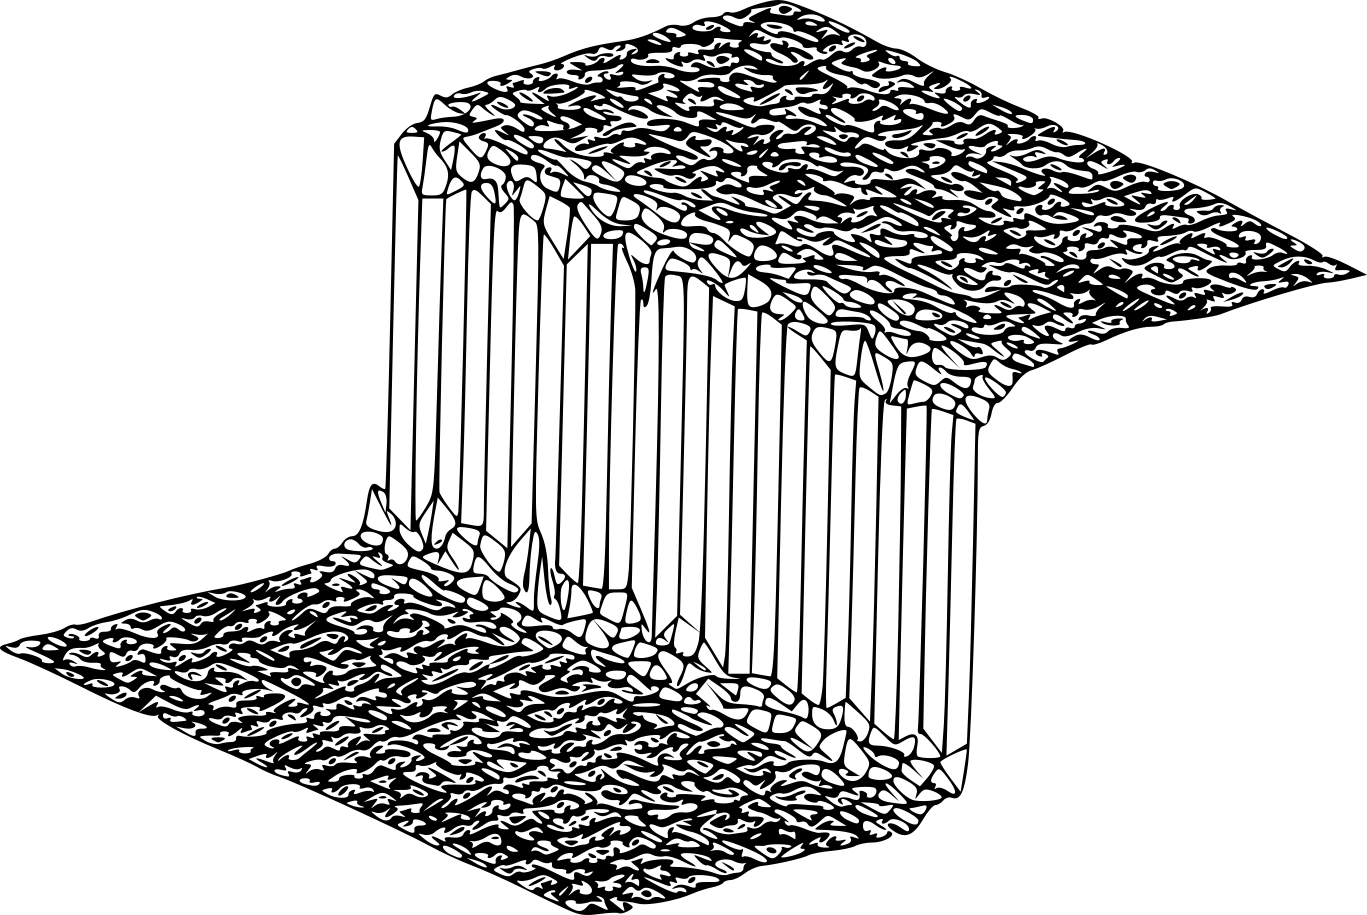
\includegraphics[width=\linewidth]{chapter04/img/bilateral3.png}
        \caption{}\label{fig:bilateral_3}
    \end{subfigure}
    \caption[Bilateral filtering visualized]{\emph{Bilateral filtering visualized.} The figures show how the bilateral filter works on a single channel step function. Figure~\ref{fig:bilateral_1} shows the original signal with random noise added. The weighting of its neighbouring pixels is computed for a pixel in the center. The weights are visualized in Figure~\ref{fig:bilateral_2}. The lower values of the step are neglected due to their lack of similarity regardless of closeness. Figure~\ref{fig:bilateral_3} shows the result of the full convolution of the filter, yielding a smoothed signal without blurred edge.}\label{fig:bilateral_filter}
\end{figure}
The filter is dependant on the functions for \emph{similarity} and \emph{closeness} and the available parameters are defined through these functions.
The Gaussian case is controlled by the parameters $\sigma_d$, the standard deviation of \emph{closeness} and $\sigma_r$, the standard deviation of \emph{similarity}.
The mathematical formulation --- based on the original publication\cite{tomasi_iccv98} --- for the \emph{closeness}~$c$ in the Gaussian case of the bilateral filter is:
\begin{equation}
\begin{aligned}
    c(\xi, \vec{x})&= \exp\left(-\frac{1}{2}{\left(\frac{d(\xi, \vec{x})}{\sigma_d} \right)}^2 \right) \\
    d(\xi, \vec{x})&= d(\xi - \vec{x}) = \lnorm{\xi - \vec{x}} \text{.}
\end{aligned}
\end{equation}
This weighs any point's $\xi$ relevance from the input signal to the filtered point $\vec{x}$ based on it's distance.
The definition of the \emph{similarity}~$s$ follows the same principle:
\begin{equation}
\begin{aligned}
    s(\xi, \vec{x})&= \exp\left(-\frac{1}{2}{\left(\frac{\theta(\mathbf{f}(\xi), \mathbf{f}(\vec{x}))}{\sigma_r}\right)}^2\right) \\
    \theta(\phi, \mathbf{f})&= \theta(\phi - \mathbf{f}) = \lnorm{\phi - \mathbf{f}}\text{.}
\end{aligned}
\end{equation}
The function $\mathbf{f}(\vec{x})$ is the value of the signal at the position $\vec{x}$ and $\theta(\phi, \mathbf{f})$ weighs these values based on their Euclidean distance.
To compute the filtered value on any point $\vec{x}$, these functions need to be applied to the whole signal.
The continuous formulation is given here, but the filter is a discrete convolution for images.
\begin{equation}
\begin{aligned}
    h(\vec{x}) &= \frac{1}{k(\vec{x})} \int_{-\infty}^{\infty} \int_{-\infty}^{\infty} \mathbf{f}(\xi) c(\xi, \vec{x}) s(\mathbf{f}(\xi), \mathbf{f}(\vec{x})) d\xi \\
    \text{with the normalization:} \\
    k(\vec{x}) &= \int_{-\infty}^{\infty} \int_{-\infty}^{\infty} c(\xi, \vec{x}) s(\mathbf{f}(\xi), \mathbf{f}(\vec{x})) d\xi
\end{aligned}
\end{equation}
Higher values of $\sigma_d$ and $\sigma_r$ result in stronger filtering of the result.
The bilateral filter is a single pass filter, but computationally expensive and slower than median blur.

\subsection{Conversion from Depth Image to Feature Image}\label{sec:feature_images}

The conversion of depth images to feature images needs to result in a single scalar value because all keypoint detectors work on a single signal channel.
Every feature image is calculated on range data in floating point format, potentially requiring the preprocessing step presented in Section~\ref{sec:range_depth_conversion}.
The representation change from integer to floating point data does no further processing than simple type conversion.

This section introduces and develops multiple potential feature images that were considered during this thesis.
Conversions for images of the \emph{Synthetic} scene (Section~\ref{sec:dataset_synthetic}), containing different primitive geometric structures, serve as examples for the visual appeal of each feature image type.

\subsubsection{Bearing-Angle Image}

\begin{figure}[H]
    \centering
    \scalebox{0.9}{%
    

\tikzset{every picture/.style={line width=0.75pt}} %set default line width to 0.75pt        

\begin{tikzpicture}[x=0.75pt,y=0.75pt,yscale=-1,xscale=1]
%uncomment if require: \path (0,228); %set diagram left start at 0, and has height of 228

%Straight Lines [id:da05017383740499093] 
\draw    (42.83,15.67) -- (145.83,202.67) ;
%Straight Lines [id:da6895513561877372] 
\draw    (205.83,46.67) -- (145.83,202.67) ;
%Curve Lines [id:da10253757735662583] 
\draw [color={rgb, 255:red, 0; green, 0; blue, 0 }  ,draw opacity=1 ]   (113,143) .. controls (119.83,127.67) and (157.83,120.67) .. (168.83,143.67) ;
%Straight Lines [id:da3851492122035306] 
\draw    (42.83,15.67) -- (205.83,46.67) ;
%Curve Lines [id:da7052636563383052] 
\draw [color={rgb, 255:red, 208; green, 2; blue, 27 }  ,draw opacity=1 ]   (166.83,39.17) .. controls (159.83,61.17) and (170.9,81.48) .. (190.9,85.48) ;
%Shape: Circle [id:dp08101382020617043] 
\draw  [fill={rgb, 255:red, 0; green, 0; blue, 0 }  ,fill opacity=1 ] (201.88,46.67) .. controls (201.88,44.49) and (203.65,42.72) .. (205.83,42.72) .. controls (208.01,42.72) and (209.78,44.49) .. (209.78,46.67) .. controls (209.78,48.85) and (208.01,50.62) .. (205.83,50.62) .. controls (203.65,50.62) and (201.88,48.85) .. (201.88,46.67) -- cycle ;
%Shape: Circle [id:dp7397482298206297] 
\draw  [fill={rgb, 255:red, 0; green, 0; blue, 0 }  ,fill opacity=1 ] (38.88,15.67) .. controls (38.88,13.49) and (40.65,11.72) .. (42.83,11.72) .. controls (45.01,11.72) and (46.78,13.49) .. (46.78,15.67) .. controls (46.78,17.85) and (45.01,19.62) .. (42.83,19.62) .. controls (40.65,19.62) and (38.88,17.85) .. (38.88,15.67) -- cycle ;

% Text Node
\draw (143,158) node  [color={rgb, 255:red, 0; green, 0; blue, 0 }  ,opacity=1 ] [align=left] {$\displaystyle \Delta $$\displaystyle \varphi $};
% Text Node
\draw (185,58) node  [color={rgb, 255:red, 208; green, 2; blue, 27 }  ,opacity=1 ] [align=left] {$\displaystyle \beta $};
% Text Node
\draw (202,110) node   [align=left] {$\displaystyle d_{i,j}$};
% Text Node
\draw (71,110) node   [align=left] {$\displaystyle d_{i-1,j}$};
% Text Node
\draw (231,46) node   [align=left] {$\displaystyle \mathbf{P}_{i,j}$};
% Text Node
\draw (16.83,15) node   [align=left] {$\displaystyle \mathbf{P}_{i-1,j}$};
% Text Node
\draw (146,215) node   [align=left] {$\displaystyle \mathbf{C}$};


\end{tikzpicture}

%
    }
    \caption[Schematic representation of \glspl{bearing-angle}]{\emph{Schematic representation of \glspl{bearing-angle}.} This figure shows the relationship of the light rays that form the \gls{bearing-angle} $\beta$.}\label{fig:bearing_angle}
\end{figure}

Scaramuzza\cite{scaramuzza_iros2007} proposes \Glspl{bearing-angle-image} that assigns each pixel the angle $\beta$ as Figure~\ref{fig:bearing_angle} demonstrates.
This angle is spanned by the two idealized lightrays for pixels of the range image.
The neighbourhood relationship between pixels can be choosen arbitrarily resulting in four \Glspl{bearing-angle-image}, horizontal, vertical, diagonal and antidiagonal.
The second variable is the direction the angle is calculted, e.g.~for horizontal images it can be calculated from left-to-right or right-to-left.
This does not exhibit new information, because the angle of the other direction is immediatly known from the fact that the sum of the angles is $180\degree$.
Nontheless, the direction must be defined to obtain stable results.

The formula for the \gls{bearing-angle} $\beta$ is derived with the cosine theorem.
Note, that both Scaramuzza\cite{scaramuzza_iros2007} and Lin\cite{lin_easp2017} have typos in the formulae they provided.
A full derivation for the correct equation is provided in Appendix~\ref{sec:bearing_derivation}.
For the horizontal left-to-right calculation the formula is as follows.
\begin{equation}\label{eq:bearing-angle}
    \beta = \arccos%
            \frac{d_{i,j} - d_{i-1,j} \cos \Delta\varphi}%
                 {\sqrt{d_{i,j}^2 + d_{i-1,j}^2 - 2 d_{i,j} d_{i-1,j} \cos \Delta\varphi}}
\end{equation}
The angular resolution $\Delta\varphi$ between two pixels of the depth image depends on the camera model in use.
The pinhole model's angular resolution changes between pixel pairs, equirectangular image have a constant resolution.
In general, the angle $\Delta\varphi$ can be calculated with the spherical coordinates $\mathbf{P_{\mathcal{S},1}}, \mathbf{P_{\mathcal{S},2}}$ of the pixel pair $\mathbf{p_1}, \mathbf{p_2}$.
Optimized versions for the specific camera model are possible in real world applications.
\begin{equation}
\begin{aligned}
    \abs{\vec{P_{\mathcal{S},1}}} &= \abs{\vec{P_{\mathcal{S},2}}} = 1 \implies \vec{P_{\mathcal{S},1}} \cdot \vec{P_{\mathcal{S},2}} = \cos \Delta\varphi \\
    \Delta\varphi &= \arccos \vec{P_{\mathcal{S},1}} \cdot \vec{P_{\mathcal{S},2}}
\end{aligned}
\end{equation}

The \Gls{bearing-angle} is in the range $\beta \in (0, \pi)~rad$.
Linear scaling of the angle to the color depth of the target image results in a grayscale image suitable for feature extraction.
A general scaling function for an \emph{unsigned 8bit} image and arbitrary angle range follows here.
This formulation can be used for different color depths and other potential angle calculations that result in different boundary conditions.
\begin{equation}
\begin{aligned}
\label{eq:linear_scaling}
    \beta_{min} &= 0 ~& c_{min} &= 0 \\
    \beta_{max} &= \pi ~& c_{max} &= 255 \\
    \beta_{scaled} &= \floor*{c_{min} + \beta \frac{c_{max} - c_{min}}{\beta_{max} - \beta_{min}}}
\end{aligned}
\end{equation}

\subsubsection*{Characteristics}

\begin{figure}[H]
    \begin{subfigure}[t]{0.32\textwidth}
        
\includegraphics[width=\linewidth]{chapter04/img/bearing-diag-0001.png}
    \end{subfigure}
    \begin{subfigure}[t]{0.32\textwidth}
        
\includegraphics[width=\linewidth]{chapter04/img/bearing-diag-0030.png}
    \end{subfigure}
    \begin{subfigure}[t]{0.32\textwidth}
        
\includegraphics[width=\linewidth]{chapter04/img/bearing-diag-0210.png}
    \end{subfigure}
    \caption[\gls{bearing-angle-image} characteristics]{\emph{\gls{bearing-angle-image} characteristics.} The \gls{bearing-angle-image} is not invariant to rotation and viewpoint changes. This property limits its applicability for automatic registration of bigger discontinues changes of the camera pose. Each depth image was converted with the diagonal (top-left-to-bottom-right direction) implementation of the \gls{bearing-angle} formula.}\label{fig:bearing_characteristics}
\end{figure}
A deeper understanding of the \gls{bearing-angle-image} helps to understand advantages and disadvantages for its usage.
Figure~\ref{fig:bearing_characteristics} demonstrates the visual changes of a synthetic scene under certain camera transformations.

The most notable property is the lack of rotation invariance.
This follows directly from the definition of the \gls{bearing-angle}.
A triangle is build by a predefined pixel relationship.
Calculating the \gls{bearing-angle} from multiple directions could lead to some rotation stability, because rotations of $45\degree$ corresponds to a different direction of pixel neighbourhood.
\begin{figure}[H]
    \centering
    

\tikzset{every picture/.style={line width=0.75pt}} %set default line width to 0.75pt        

\begin{tikzpicture}[x=0.75pt,y=0.75pt,yscale=-1,xscale=1]
%uncomment if require: \path (0,111); %set diagram left start at 0, and has height of 111

%Shape: Arc [id:dp6607157958124017] 
\draw  [draw opacity=0] (294.74,88.39) .. controls (296.93,80.02) and (304.55,73.85) .. (313.6,73.85) .. controls (324.37,73.85) and (333.1,82.58) .. (333.1,93.35) -- (313.6,93.35) -- cycle ; \draw  [color={rgb, 255:red, 245; green, 166; blue, 35 }  ,draw opacity=1 ] (294.74,88.39) .. controls (296.93,80.02) and (304.55,73.85) .. (313.6,73.85) .. controls (324.37,73.85) and (333.1,82.58) .. (333.1,93.35) ;
%Shape: Arc [id:dp6461315771728425] 
\draw  [draw opacity=0] (107.76,82.98) .. controls (111.29,78.06) and (117.07,74.85) .. (123.6,74.85) .. controls (134.06,74.85) and (142.59,83.08) .. (143.08,93.42) -- (123.6,94.35) -- cycle ; \draw  [color={rgb, 255:red, 74; green, 144; blue, 226 }  ,draw opacity=1 ] (107.76,82.98) .. controls (111.29,78.06) and (117.07,74.85) .. (123.6,74.85) .. controls (134.06,74.85) and (142.59,83.08) .. (143.08,93.42) ;
%Straight Lines [id:da7912546873109455] 
\draw [line width=3]    (62.6,94) -- (429.6,94) ;
%Shape: Circle [id:dp6585955324129855] 
\draw  [draw opacity=0][fill={rgb, 255:red, 0; green, 0; blue, 0 }  ,fill opacity=1 ] (16,14.3) .. controls (16,11.93) and (17.93,10) .. (20.3,10) .. controls (22.67,10) and (24.6,11.93) .. (24.6,14.3) .. controls (24.6,16.67) and (22.67,18.6) .. (20.3,18.6) .. controls (17.93,18.6) and (16,16.67) .. (16,14.3) -- cycle ;
%Straight Lines [id:da6943190688257042] 
\draw    (20.3,14.3) -- (123.6,94.35) ;
%Straight Lines [id:da2008172675955413] 
\draw    (20.3,14.3) -- (171.6,93.35) ;
%Straight Lines [id:da41493445776640725] 
\draw    (20.3,14.3) -- (313.6,93.35) ;
%Straight Lines [id:da4646477074321278] 
\draw    (20.3,14.3) -- (414.6,92.35) ;

% Text Node
\draw (14,23) node [anchor=north west][inner sep=0.75pt]   [align=left] {$\displaystyle \mathbf{C}$};
% Text Node
\draw (121.6,77.35) node [anchor=north west][inner sep=0.75pt]  [font=\scriptsize,color={rgb, 255:red, 74; green, 144; blue, 226 }  ,opacity=1 ] [align=left] {$\displaystyle \beta $};
% Text Node
\draw (310.6,77.35) node [anchor=north west][inner sep=0.75pt]  [font=\scriptsize,color={rgb, 255:red, 245; green, 166; blue, 35 }  ,opacity=1 ] [align=left] {$\displaystyle \beta '$};


\end{tikzpicture}

%
    \caption[Two \glspl{bearing-angle} for the same ground plane]{\emph{Two \glspl{bearing-angle} for the same ground plane.} Different shadings of plane surfaces depend on the perspective projection and the distance from the camera center $C$ to the surface.}\label{fig:bearing_angle_shading}
\end{figure}
The second apparent aspect is the change in shading for example the flat ground, but other surfaces as well.
This effect is due to the perspective transformation and the distance of a point to the camera, as Figure~\ref{fig:bearing_angle_shading} demonstrates.
Round objects, like spheres, experience no visual change in shading.
The triangles of the lightrays are invariant to camera transformation for such objects.

\subsubsection{Multi-Directional Bearing Angle}

The \emph{Multi-Directional \gls{bearing-angle-image}} attempts to overcome the limitation of missing rotation invariance for the classical \gls{bearing-angle-image}.
Instead of just one angle in one direction, the two adjacent triangle are analyzed together.
Figure~\ref{fig:max-curve} shows how the triangles are related.
Both angles $\beta$ and $\gamma$ are calculated with equation~\ref{eq:bearing-angle}, for $\gamma$ the values of $d_{i,j}$ and $d_{i-1,j}$ just need to be swapped.
\begin{figure}
    

\tikzset{every picture/.style={line width=0.75pt}} %set default line width to 0.75pt        

\begin{tikzpicture}[x=0.75pt,y=0.75pt,yscale=-1,xscale=1]
%uncomment if require: \path (0,252); %set diagram left start at 0, and has height of 252

%Straight Lines [id:da05017383740499093] 
\draw    (46.83,26.67) -- (149.83,213.67) ;
%Straight Lines [id:da6895513561877372] 
\draw    (155.83,32.67) -- (149.83,213.67) ;
%Curve Lines [id:da10253757735662583] 
\draw [color={rgb, 255:red, 0; green, 0; blue, 0 }  ,draw opacity=1 ]   (116,153) .. controls (128.83,126.67) and (169.83,125.67) .. (181.83,145.67) ;
%Straight Lines [id:da3851492122035306] 
\draw    (46.83,26.67) -- (155.83,32.67) ;
%Shape: Circle [id:dp08101382020617043] 
\draw  [fill={rgb, 255:red, 0; green, 0; blue, 0 }  ,fill opacity=1 ] (151.88,32.67) .. controls (151.88,30.49) and (153.65,28.72) .. (155.83,28.72) .. controls (158.01,28.72) and (159.78,30.49) .. (159.78,32.67) .. controls (159.78,34.85) and (158.01,36.62) .. (155.83,36.62) .. controls (153.65,36.62) and (151.88,34.85) .. (151.88,32.67) -- cycle ;
%Shape: Circle [id:dp7397482298206297] 
\draw  [fill={rgb, 255:red, 0; green, 0; blue, 0 }  ,fill opacity=1 ] (42.88,26.67) .. controls (42.88,24.49) and (44.65,22.72) .. (46.83,22.72) .. controls (49.01,22.72) and (50.78,24.49) .. (50.78,26.67) .. controls (50.78,28.85) and (49.01,30.62) .. (46.83,30.62) .. controls (44.65,30.62) and (42.88,28.85) .. (42.88,26.67) -- cycle ;
%Shape: Circle [id:dp7936487176657823] 
\draw  [fill={rgb, 255:red, 0; green, 0; blue, 0 }  ,fill opacity=1 ] (241.88,7.67) .. controls (241.88,5.49) and (243.65,3.72) .. (245.83,3.72) .. controls (248.01,3.72) and (249.78,5.49) .. (249.78,7.67) .. controls (249.78,9.85) and (248.01,11.62) .. (245.83,11.62) .. controls (243.65,11.62) and (241.88,9.85) .. (241.88,7.67) -- cycle ;
%Straight Lines [id:da7225304487809803] 
\draw    (245.83,7.67) -- (149.83,213.67) ;
%Straight Lines [id:da15289701870660388] 
\draw    (155.83,32.67) -- (245.83,7.67) ;
%Shape: Arc [id:dp845909277560968] 
\draw  [draw opacity=0] (154.29,72.43) .. controls (153.16,72.54) and (152.02,72.6) .. (150.87,72.6) .. controls (131.56,72.6) and (115.9,56.94) .. (115.9,37.63) .. controls (115.9,35.08) and (116.17,32.59) .. (116.69,30.19) -- (150.87,37.63) -- cycle ; \draw  [color={rgb, 255:red, 208; green, 2; blue, 27 }  ,draw opacity=1 ] (154.29,72.43) .. controls (153.16,72.54) and (152.02,72.6) .. (150.87,72.6) .. controls (131.56,72.6) and (115.9,56.94) .. (115.9,37.63) .. controls (115.9,35.08) and (116.17,32.59) .. (116.69,30.19) ;
%Shape: Arc [id:dp15343497156889918] 
\draw  [draw opacity=0] (193.67,22.29) .. controls (195.16,26.33) and (195.97,30.7) .. (195.97,35.25) .. controls (195.97,55.99) and (179.15,72.8) .. (158.42,72.8) .. controls (157.06,72.8) and (155.72,72.73) .. (154.4,72.59) -- (158.42,35.25) -- cycle ; \draw  [color={rgb, 255:red, 245; green, 166; blue, 35 }  ,draw opacity=1 ] (193.67,22.29) .. controls (195.16,26.33) and (195.97,30.7) .. (195.97,35.25) .. controls (195.97,55.99) and (179.15,72.8) .. (158.42,72.8) .. controls (157.06,72.8) and (155.72,72.73) .. (154.4,72.59) ;

% Text Node
\draw (137,154) node  [color={rgb, 255:red, 0; green, 0; blue, 0 }  ,opacity=1 ] [align=left] {$\displaystyle \Delta $$\displaystyle \varphi $};
% Text Node
\draw (138,48) node  [color={rgb, 255:red, 208; green, 2; blue, 27 }  ,opacity=1 ] [align=left] {$\displaystyle \beta $};
% Text Node
\draw (169,100) node   [align=left] {$\displaystyle d_{i,j}$};
% Text Node
\draw (65,100) node   [align=left] {$\displaystyle d_{i-1,j}$};
% Text Node
\draw (154,12) node   [align=left] {$\displaystyle \mathbf{P}_{i,j}$};
% Text Node
\draw (150,226) node   [align=left] {$\displaystyle \mathbf{C}$};
% Text Node
\draw (232,99) node   [align=left] {$\displaystyle d_{i+1,j}$};
% Text Node
\draw (172,48) node   [align=left] {$\displaystyle \textcolor[rgb]{0.96,0.65,0.14}{\gamma }$};
% Text Node
\draw (165,154) node  [color={rgb, 255:red, 0; green, 0; blue, 0 }  ,opacity=1 ] [align=left] {$\displaystyle \Delta $$\displaystyle \theta $};
% Text Node
\draw (273,12) node   [align=left] {$\displaystyle \mathbf{P}_{i+1,j}$};
% Text Node
\draw (24,12) node   [align=left] {$\displaystyle \mathbf{P}_{i-1,j}$};


\end{tikzpicture}


    \caption[Schematic Representation of the Multi-Directional \gls{bearing-angle-image}]{The Multi-Directional \gls{bearing-angle-image} composes two \Glspl{bearing-angle} in vertical, horizontal, diagonal and antidiagonal direction. The maximum angle is then selected as pixel value.}\label{fig:max-curve}
\end{figure}
Both angles are added together, resulting in the angle of an edge at this position.
\begin{equation}
    \mathcal{B} = \beta + \gamma
\end{equation}
This calculation is again only in one direction and not rotation invariant but already symmetrical.
The value $B$ can be defined for diagonal, antidiagonal, horizontal and vertical sampling of the image.
The final step for rotation invariance is the reduction of these four values to its maximum.
\begin{align}
    \mathcal{B} &= \max{\{\mathcal{B}_{diagonal}, \mathcal{B}_{antidiagonal}, \mathcal{B}_{horizontal}, \mathcal{B}_{vertical}\}}
\end{align}
The converted images in Figure~\ref{fig:max-curve-images} show the same scene and positions as for the \gls{bearing-angle-image}.
\begin{figure}[H]
    \begin{subfigure}[t]{0.32\textwidth}
        
\includegraphics[width=\linewidth]{chapter04/img/max-0001.png}
    \end{subfigure}
    \begin{subfigure}[t]{0.32\textwidth}
        
\includegraphics[width=\linewidth]{chapter04/img/max-0030.png}
    \end{subfigure}
    \begin{subfigure}[t]{0.32\textwidth}
        
\includegraphics[width=\linewidth]{chapter04/img/max-0210.png}
    \end{subfigure}
    \caption{The subfigures show the same camera positions as the \gls{bearing-angle} and demonstrates the rotation invariance. Each edge in the geometry forms a visible white line. No other textures exist.}\label{fig:max-curve-images}
\end{figure}
The goal of rotational invariance is achieved, unfortunatly the image lacks texture and contrast.
Qualitative tests with common feature detectors yielded weak keypoint responses.
Therefore, this approach received no further attention.

\subsubsection{Curvature Image}

Differential geometry provides a scalar quantity assignable to each point of a one-dimensional differntiable function, the \emph{\gls{curvature}} $\kappa$\cite[p. 10]{Kuhnel2008}.
This concept can be generalized to higher dimensions and two common \glspl{curvature} exist for surfaces in three-dimensional space, \emph{\gls{gaussian-curvature}} and \emph{\gls{mean-curvature}}.
\begin{figure}[t]
    \begin{subfigure}[t]{0.48\textwidth}
        \centering
        \scalebox{0.85}{%
        \begin{tikzpicture}
\begin{axis}[xmin=-0.7,
             xmax=0.7,
             ymin=-0.1,
             ymax=1.1,
             samples=200,
             axis line style={draw=none},
             tick style={draw=none},
             xticklabels={\empty},
             yticklabels={\empty},
             grid=major,
             plot box ratio={2 1},
             axis equal]
    \draw[plotorange, line width=1.3pt] (axis cs:0,0.5) circle [radius=50];
    \addplot[plotblue, line width=1.5pt] {x*x};
    \coordinate (C) at (axis cs:{0.0,0.5});
    \coordinate (O) at (axis cs:{0.0,0.0});
    \coordinate (L) at (axis cs:{0.1,0.25});
    \node at (L) {$\mathbf{r}$};
    \node[label={90:{$\mathbf{C}$}},circle,fill,inner sep=1pt] at (C) {};
    \draw[thick,-](C)--(O);
\end{axis}
\end{tikzpicture}

        }
        \caption{The \gls{curvature} of a line at a specific point is defined by its osculating circle.}\label{fig:osculating_circle}
    \end{subfigure}\hfill%
    \begin{subfigure}[t]{0.48\textwidth}
        \centering
        \scalebox{0.85}{%
        \begin{tikzpicture}
\begin{axis}[xmin=-1.0,xmax=1.0,
             ymin=-1.0,ymax=1.0,
             zmin=-1.0,zmax=1.0,
             grid=major,
             axis line style={draw=none},
             tick style={draw=none},
             view={310}{35},
             xticklabels={\empty},
             yticklabels={\empty},
             zticklabels={\empty},
             plot box ratio={1 1 3},
             colormap/redyellow]
\newcommand\func[2]{#1^3 - #2^2}
\definecolor{darkorange}{HTML}{84644B}

    \addplot3[surf,
              shader=faceted interp,
              faceted color={darkorange},
              samples=15,
              domain=-1:1,
              y domain=-1:1] {\func{x}{y}};

    % plot curve for x direction
    \addplot3[samples=15,
              domain=-1:1,
              samples y=1,
              dotted,
              black,
              line width=1.1pt,
              smooth] (x, 0, \func{x}{0});
    % plot curve for y direction
    \addplot3[samples=15,
              domain=-1:1,
              y domain=-1:0.22,
              dotted,
              black,
              line width=1.1pt,
              smooth] (0, y, \func{0}{y});
\end{axis}
\end{tikzpicture}

        }
        \caption{The principal curvatures are the maximum and minimum \glspl{curvature} in all directions.}\label{fig:curvature_surface}
    \end{subfigure}
    \caption[Curvature of curves and surfaces]{\emph{Curvature of curves and surfaces.} The \gls{curvature} of a curve is defined through its osculating circle. This simple definition is not possible for surfaces in three dimensions. Analyzing all directions, each point on the surface does have a minimum and maximum \gls{curvature} --- the \emph{principal curvatures}.}
\end{figure}
A straight line has no \gls{curvature}, hence $\kappa = 0$.
The \gls{curvature} of a circle is defined is the inverse of its radius
\begin{equation}
    \kappa_{circle} = \frac{1}{r}\text{.}
\end{equation}
Any point's \gls{curvature} on a one-dimensional, twice differentiable function is defined as the \gls{curvature} of its osculating circle, visualized in Figure~\ref{fig:osculating_circle}.
The \gls{curvature} of any point of a surface in three-dimensional space is ambigous, because it has infinite many curves crossing through this point.
But a maximum and minimum \gls{curvature} exist, the \emph{principal curvatures} $k_1$ and $k_2$.
Figure~\ref{fig:curvature_surface} visualizes the directions of the minimum and maximum \gls{curvature} of a surface in three-dimensional space as dotted black lines.
The \emph{\Gls{gaussian-curvature}} $\mathcal{K}$ is defined as the product
\begin{equation}
    \mathcal{K} = k_1 k_2
\end{equation}
and the \emph{\gls{mean-curvature}} $\mathcal{H}$ as the mean
\begin{equation}
    \mathcal{H} = \frac{1}{2} (k_1 k_2)
\end{equation}
of the principal curvatures.

Both quantities can be calculated differently, as the \gls{curvature} is related to the derivates of a function.
Let $f(u, v)$ be a two-dimensional function representing the depth image and $f_u$, $f_v$, $f_{uu}$ and $f_{vv}$ its partial derivatives.
Then the \gls{gaussian-curvature} and \gls{mean-curvature} are computed with:
\begin{equation}
\begin{aligned}
    \mathcal{K} &= \frac{f_{uu} f_{vv} - f_{uv}^2}{{(1 + f_u^2 + f_v^2)}^2}\text{,} \\
    \mathcal{H} &= \frac{{(1 + f_{v}^2)} f_{uu} - 2 f_u f_v f_{uv} + {(1 + f_u^2)} f_{vv}}{2 \sqrt{1 + f_u^2 + f_v^2}^3}\text{.}
\end{aligned}
\end{equation}
The central differential quotients approximate the first and second derivatives with $\mathcal{O}(\Delta x^2)$ accuracy:
\begin{equation}
\begin{aligned}
    f_{x} &= \frac{y_{i+1} - y_{i-1}}{2 \Delta x} \\
    f_{xx} &= \frac{y_{i+1} + y_{i-1} - 2 y_{i}}{{\Delta x}^2}\text{.}
\end{aligned}
\end{equation}

\begin{figure}[tb]
    \begin{subfigure}[t]{0.32\textwidth}
        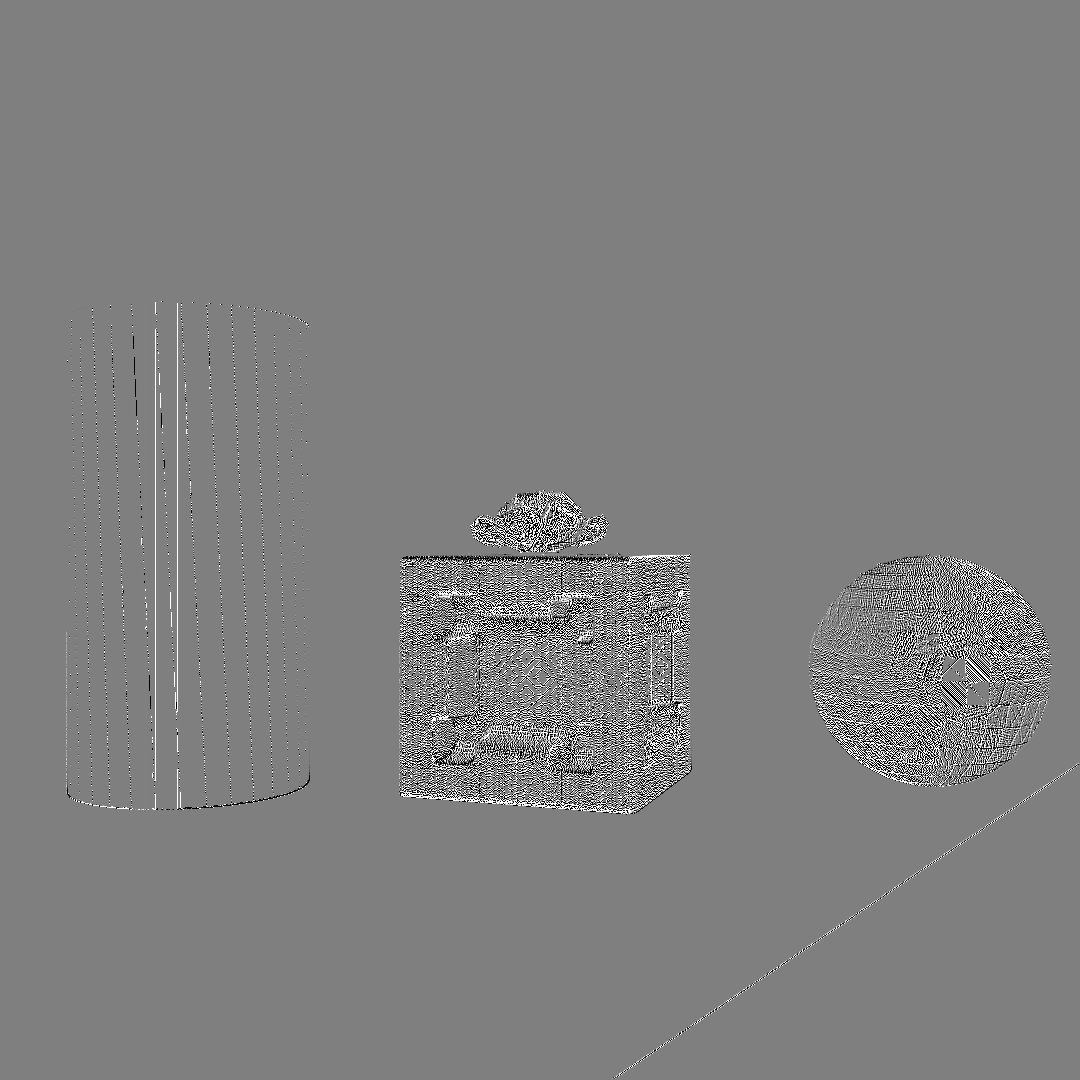
\includegraphics[width=\linewidth]{chapter04/img/mean-0001.png}
    \end{subfigure}
    \begin{subfigure}[t]{0.32\textwidth}
        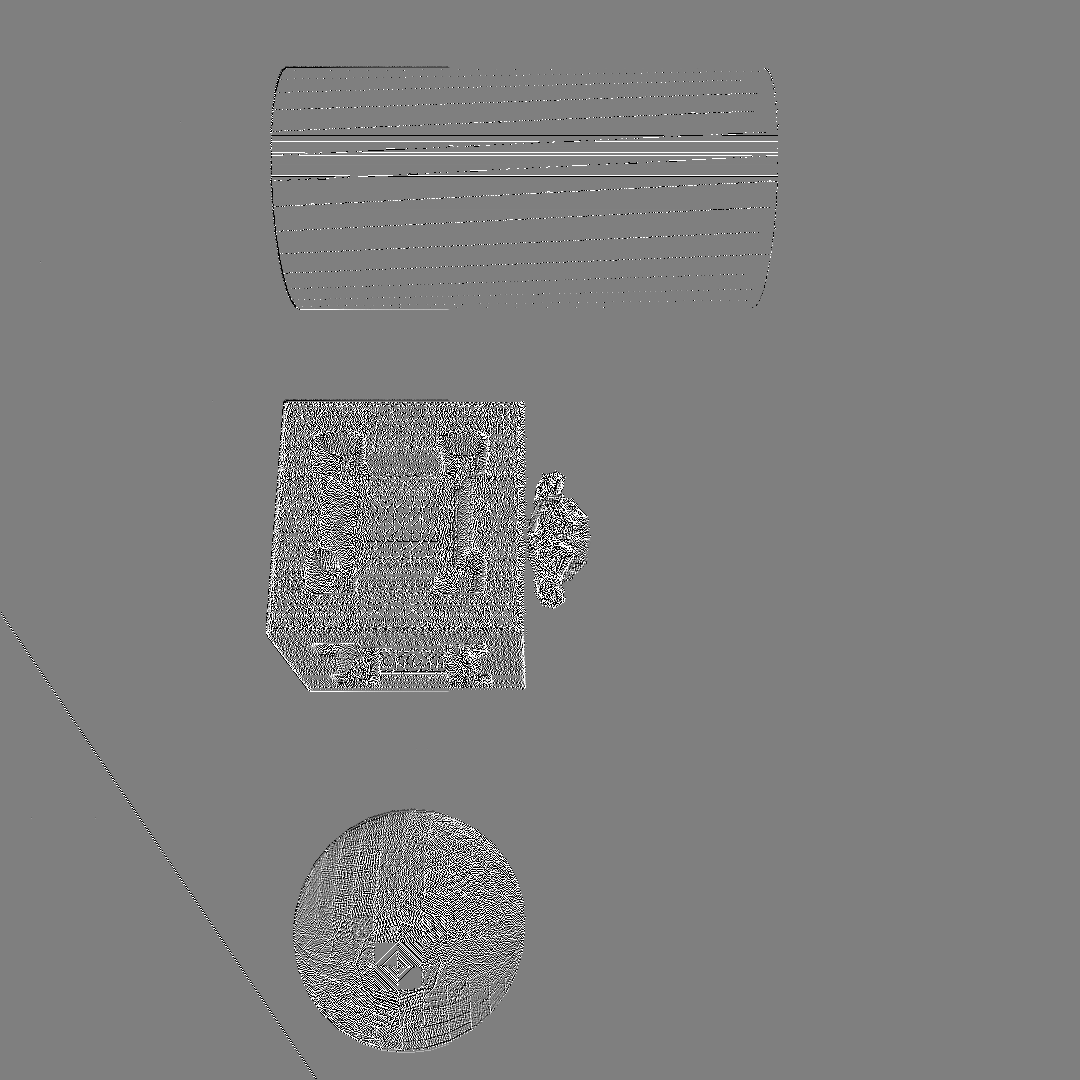
\includegraphics[width=\linewidth]{chapter04/img/mean-0030.png}
    \end{subfigure}
    \begin{subfigure}[t]{0.32\textwidth}
        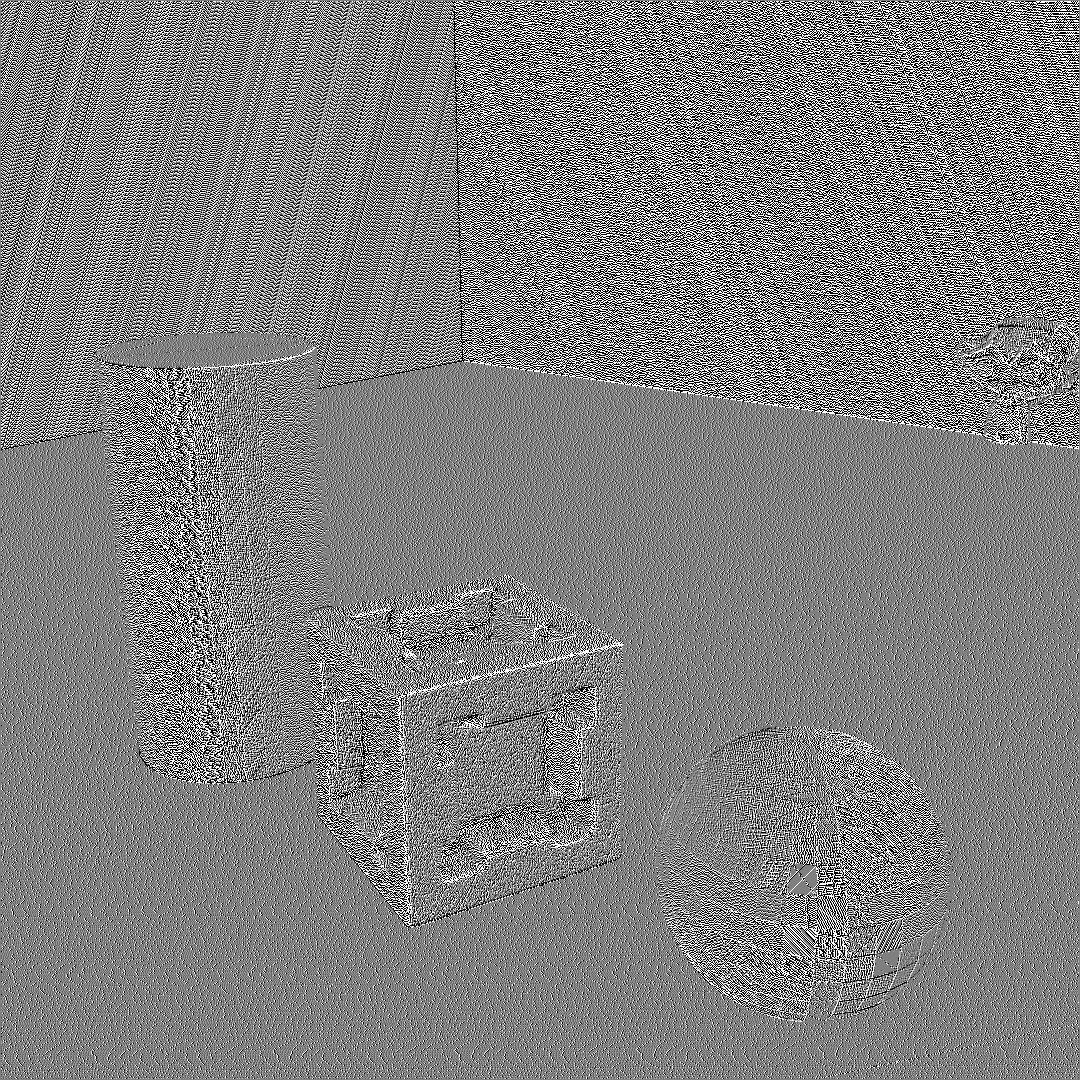
\includegraphics[width=\linewidth]{chapter04/img/mean-0210.png}
    \end{subfigure}
    \caption[\Gls{mean-curvature} in the \emph{Synthetic} scene]{\emph{\Gls{mean-curvature} in the Synthetic scene.} The \gls{mean-curvature} feature image for the same synthetic scene are similar to Multi-Directional \Glspl{bearing-angle-image}, making them a second non-promising option.}\label{fig:mean-curvature}
\end{figure}
The result of the \gls{mean-curvature} conversion in Figure~\ref{fig:mean-curvature} is similar to the Multi-Directional \gls{bearing-angle-image}.
The \gls{mean-curvature} is rotation invariant but the result is already very unstable to the noise induced by integer precision depth images.
Figure~\ref{fig:gaussian-curvature} shows the images for the \gls{gaussian-curvature}.
It is even more prone to noise in the input and suffers from the same range issue.

Both the \gls{mean-curvature} and \gls{gaussian-curvature} are unbound and result in any real number.
Simple scaling between the computed minimum and maximum value is unstable between images and results in completly gray images as these quantities have noticable outliers.
As solution for this problem the computed values are clamped to a predefined range, for example $\mathcal{H},\mathcal{K} \in (-20, 20)$ and then scaled to the desired image depth of the feature image.
\begin{figure}[tb]
    \begin{subfigure}[t]{0.32\textwidth}
        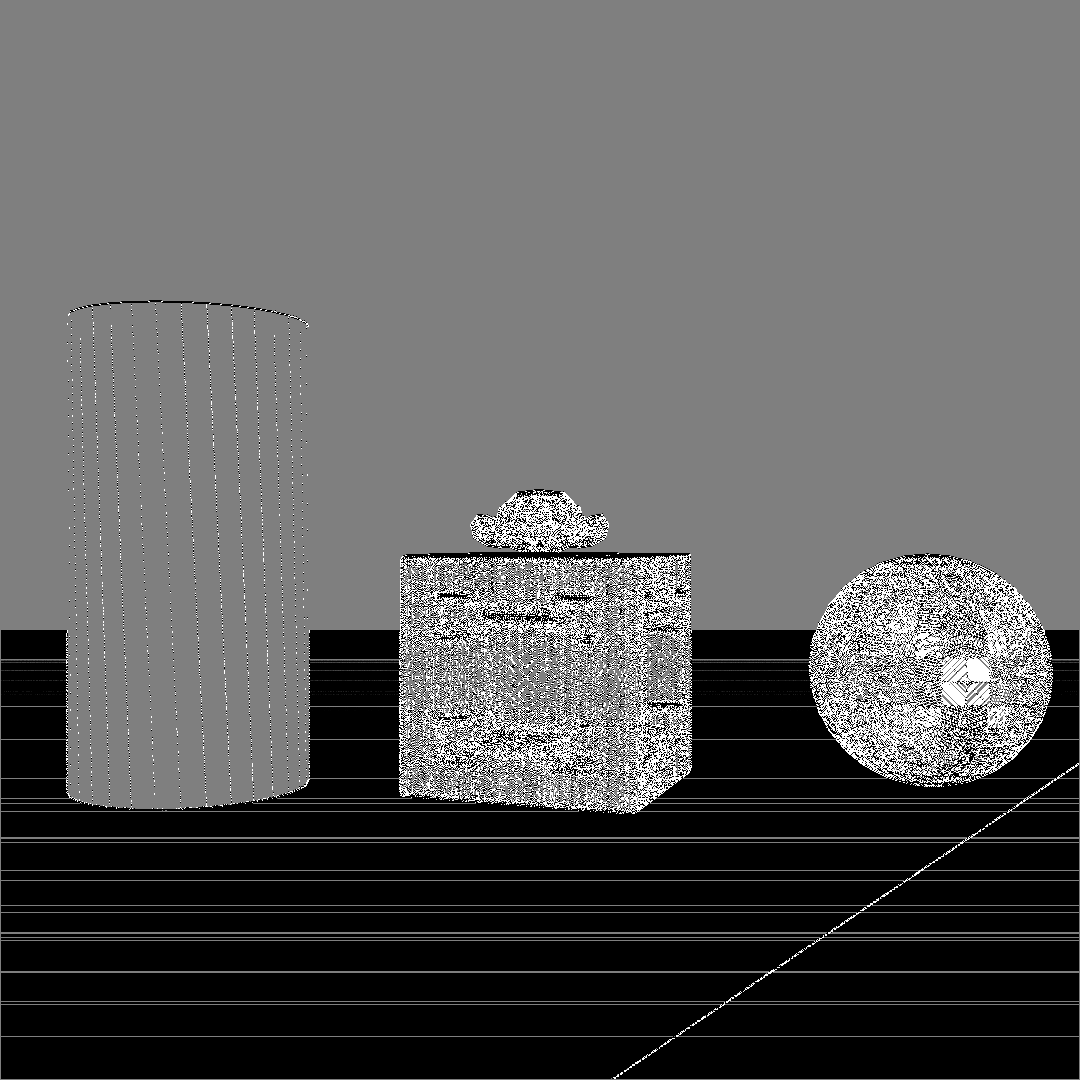
\includegraphics[width=\linewidth]{chapter04/img/gauss-0001.png}
    \end{subfigure}
    \begin{subfigure}[t]{0.32\textwidth}
        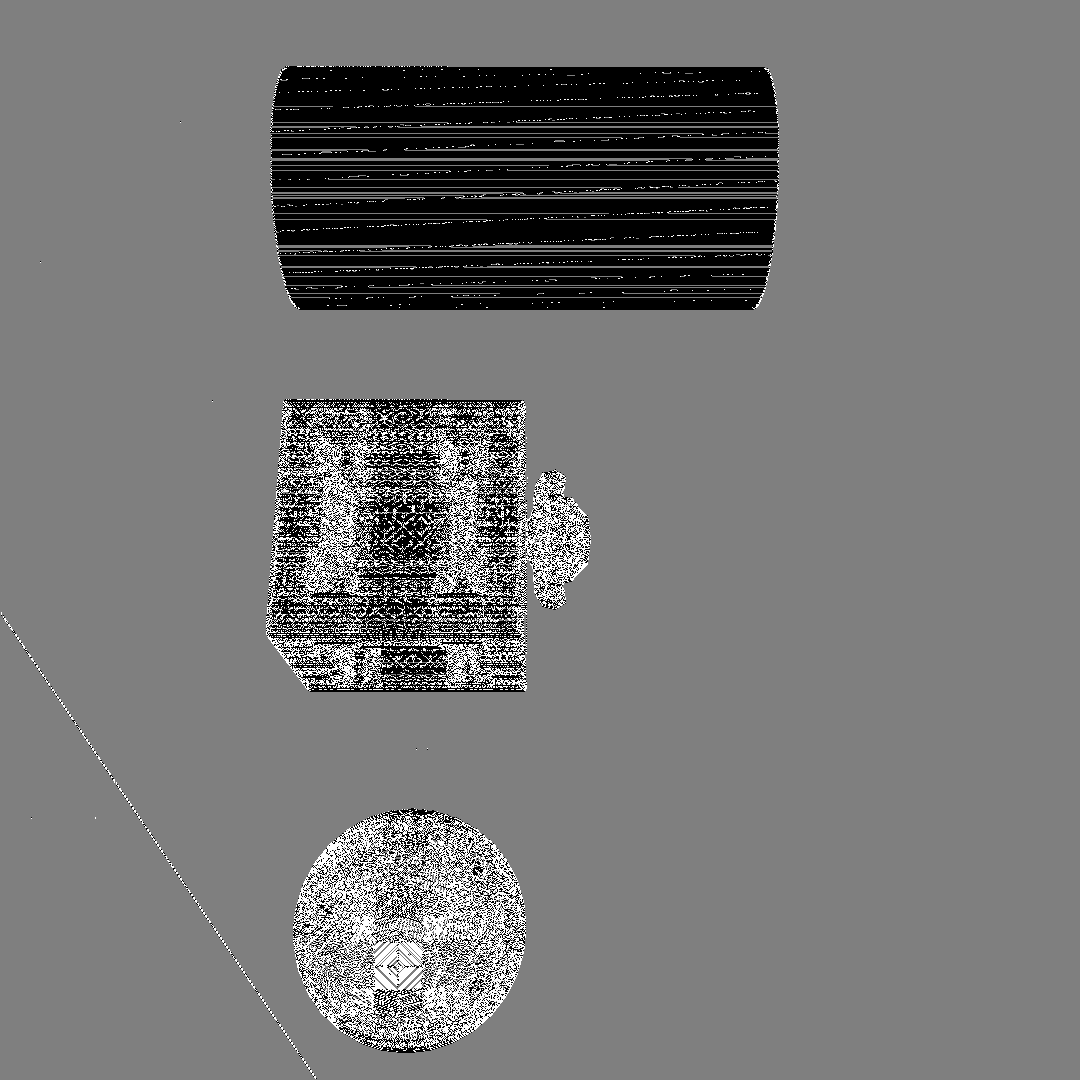
\includegraphics[width=\linewidth]{chapter04/img/gauss-0030.png}
    \end{subfigure}
    \begin{subfigure}[t]{0.32\textwidth}
        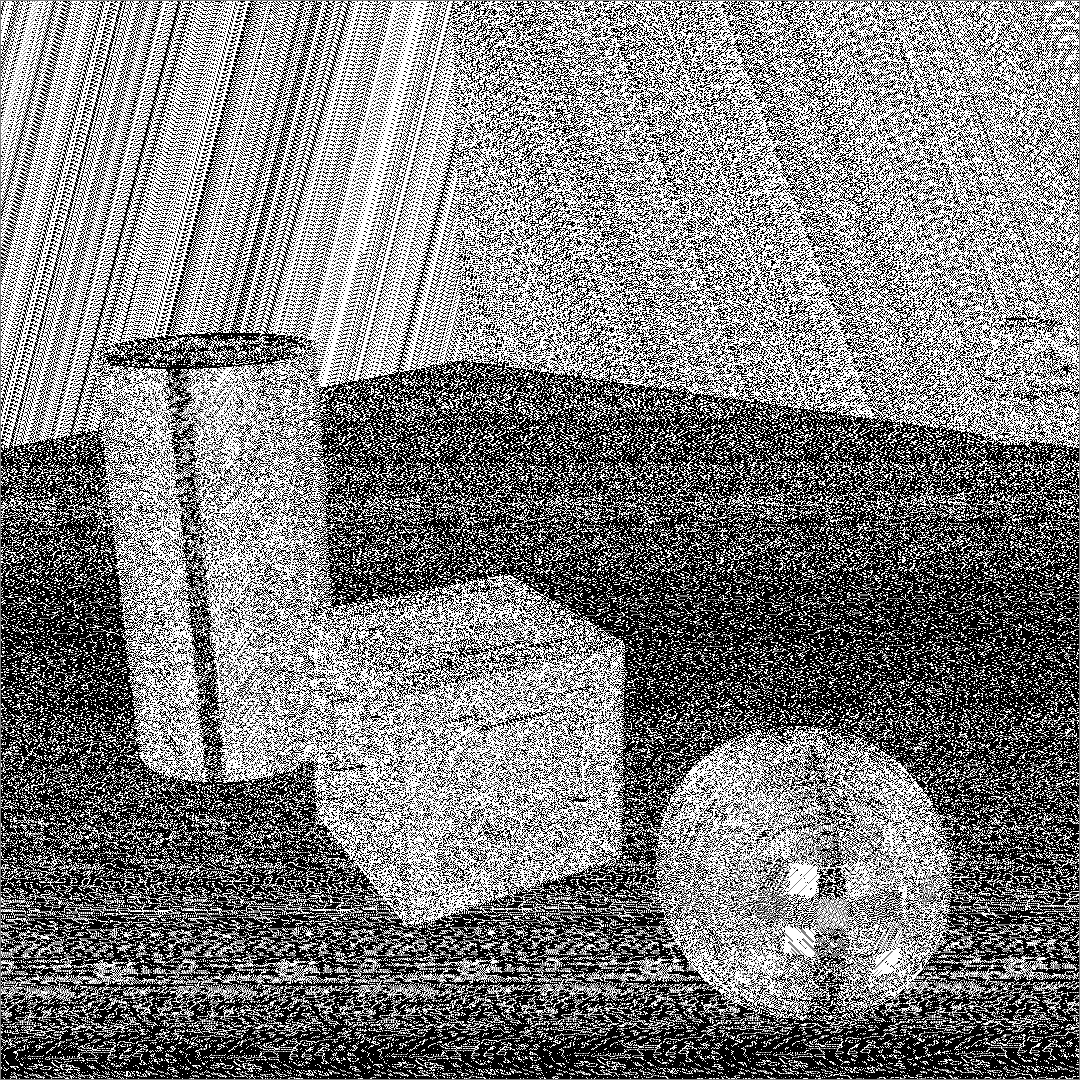
\includegraphics[width=\linewidth]{chapter04/img/gauss-0210.png}
    \end{subfigure}
    \caption[\Gls{gaussian-curvature} in the \emph{Synthetic} scene]{\emph{\Gls{gaussian-curvature} in the Synthetic scene.} The \Gls{gaussian-curvature} feature images for the synthetic scene. The results are not promising either.}\label{fig:gaussian-curvature}
\end{figure}
Computing the curvature for the whole image has the theoretical weakness, that discontinuities at object boundaries are not respected.
The derivatives do not exist at these points for perfect depth sensing.
A mathematically accurate computation requires object identification or meshing of the scene.
Such a requirement seems unreasonable for a foundational processing step in potential real-time use cases.

\subsubsection{\Glspl{flexion-image}}\label{flexion-image-section}

The local shape of an object that is sampled by a depth sensor is characterized by its normalized surface normal.
A surface normal is a vector perpendicular to the surface of the object.
This characterization builds the foundation of the \Gls{flexion-image} and its inspiration, too.

Each measured pixel is backprojected to camera coordinates, scaling the point in spherical coordinates with its measured range, as first step.
Approximating the normal for a measured surface point $\mathbf{P_{i,j}}$ is possible using the cross product of its neighbours connecting vectors.
The point relationship is visualized in Figure~\ref{fig:flexion_normals_plane}.
\begin{figure}[H]
    \begin{subfigure}[t]{0.49\linewidth}
        \centering
        \scalebox{1.0}{%
        

\tikzset{every picture/.style={line width=0.75pt}} %set default line width to 0.75pt        

\begin{tikzpicture}[x=0.75pt,y=0.75pt,yscale=-1,xscale=1]
%uncomment if require: \path (0,237); %set diagram left start at 0, and has height of 237

%Shape: Rectangle [id:dp6565487036659107] 
\draw  [color={rgb, 255:red, 155; green, 155; blue, 155 }  ,draw opacity=1 ][dash pattern={on 4.5pt off 4.5pt}] (28.7,13.7) -- (206.3,13.7) -- (206.3,191.3) -- (28.7,191.3) -- cycle ;
%Straight Lines [id:da30195081571029425] 
\draw [color={rgb, 255:red, 74; green, 144; blue, 226 }  ,draw opacity=1 ] [dash pattern={on 4.5pt off 4.5pt}]  (28.7,102.5) -- (206.3,102.5) ;
%Straight Lines [id:da4586174781414081] 
\draw [color={rgb, 255:red, 74; green, 144; blue, 226 }  ,draw opacity=1 ] [dash pattern={on 4.5pt off 4.5pt}]  (117.5,13.7) -- (117.5,191.3) ;
%Straight Lines [id:da7294828306266232] 
\draw [color={rgb, 255:red, 245; green, 166; blue, 35 }  ,draw opacity=1 ] [dash pattern={on 4.5pt off 4.5pt}]  (28.7,13.7) -- (206.3,191.3) ;
%Straight Lines [id:da3243995266948473] 
\draw [color={rgb, 255:red, 245; green, 166; blue, 35 }  ,draw opacity=1 ] [dash pattern={on 4.5pt off 4.5pt}]  (28.7,191.3) -- (206.3,13.7) ;
%Shape: Circle [id:dp5266363779447065] 
\draw  [fill={rgb, 255:red, 245; green, 166; blue, 35 }  ,fill opacity=1 ] (25,13.7) .. controls (25,11.66) and (26.66,10) .. (28.7,10) .. controls (30.74,10) and (32.4,11.66) .. (32.4,13.7) .. controls (32.4,15.74) and (30.74,17.4) .. (28.7,17.4) .. controls (26.66,17.4) and (25,15.74) .. (25,13.7) -- cycle ;
%Shape: Ellipse [id:dp14497174740803043] 
\draw  [fill={rgb, 255:red, 74; green, 144; blue, 226 }  ,fill opacity=1 ] (25,102.5) .. controls (25,100.46) and (26.66,98.8) .. (28.7,98.8) .. controls (30.74,98.8) and (32.4,100.46) .. (32.4,102.5) .. controls (32.4,104.54) and (30.74,106.2) .. (28.7,106.2) .. controls (26.66,106.2) and (25,104.54) .. (25,102.5) -- cycle ;
%Shape: Ellipse [id:dp0427609892023727] 
\draw  [fill={rgb, 255:red, 245; green, 166; blue, 35 }  ,fill opacity=1 ] (25,191.3) .. controls (25,189.26) and (26.66,187.6) .. (28.7,187.6) .. controls (30.74,187.6) and (32.4,189.26) .. (32.4,191.3) .. controls (32.4,193.34) and (30.74,195) .. (28.7,195) .. controls (26.66,195) and (25,193.34) .. (25,191.3) -- cycle ;
%Shape: Ellipse [id:dp2872052196845898] 
\draw  [fill={rgb, 255:red, 74; green, 144; blue, 226 }  ,fill opacity=1 ] (113.8,13.7) .. controls (113.8,11.66) and (115.46,10) .. (117.5,10) .. controls (119.54,10) and (121.2,11.66) .. (121.2,13.7) .. controls (121.2,15.74) and (119.54,17.4) .. (117.5,17.4) .. controls (115.46,17.4) and (113.8,15.74) .. (113.8,13.7) -- cycle ;
%Shape: Circle [id:dp758793708555806] 
\draw  [fill={rgb, 255:red, 0; green, 0; blue, 0 }  ,fill opacity=1 ] (113.8,102.5) .. controls (113.8,100.46) and (115.46,98.8) .. (117.5,98.8) .. controls (119.54,98.8) and (121.2,100.46) .. (121.2,102.5) .. controls (121.2,104.54) and (119.54,106.2) .. (117.5,106.2) .. controls (115.46,106.2) and (113.8,104.54) .. (113.8,102.5) -- cycle ;
%Shape: Circle [id:dp477059334030714] 
\draw  [fill={rgb, 255:red, 74; green, 144; blue, 226 }  ,fill opacity=1 ] (113.8,191.3) .. controls (113.8,189.26) and (115.46,187.6) .. (117.5,187.6) .. controls (119.54,187.6) and (121.2,189.26) .. (121.2,191.3) .. controls (121.2,193.34) and (119.54,195) .. (117.5,195) .. controls (115.46,195) and (113.8,193.34) .. (113.8,191.3) -- cycle ;
%Shape: Ellipse [id:dp13207731000753575] 
\draw  [fill={rgb, 255:red, 245; green, 166; blue, 35 }  ,fill opacity=1 ] (202.6,13.7) .. controls (202.6,11.66) and (204.26,10) .. (206.3,10) .. controls (208.34,10) and (210,11.66) .. (210,13.7) .. controls (210,15.74) and (208.34,17.4) .. (206.3,17.4) .. controls (204.26,17.4) and (202.6,15.74) .. (202.6,13.7) -- cycle ;
%Shape: Circle [id:dp8288145253462365] 
\draw  [fill={rgb, 255:red, 74; green, 144; blue, 226 }  ,fill opacity=1 ] (202.6,102.5) .. controls (202.6,100.46) and (204.26,98.8) .. (206.3,98.8) .. controls (208.34,98.8) and (210,100.46) .. (210,102.5) .. controls (210,104.54) and (208.34,106.2) .. (206.3,106.2) .. controls (204.26,106.2) and (202.6,104.54) .. (202.6,102.5) -- cycle ;
%Shape: Circle [id:dp9160642610677009] 
\draw  [fill={rgb, 255:red, 245; green, 166; blue, 35 }  ,fill opacity=1 ] (202.6,191.3) .. controls (202.6,189.26) and (204.26,187.6) .. (206.3,187.6) .. controls (208.34,187.6) and (210,189.26) .. (210,191.3) .. controls (210,193.34) and (208.34,195) .. (206.3,195) .. controls (204.26,195) and (202.6,193.34) .. (202.6,191.3) -- cycle ;

% Text Node
\draw (106,110) node [anchor=north west][inner sep=0.75pt]   [align=left] {$\displaystyle \mathbf{P}_{i,j}$};
% Text Node
\draw (195,110) node [anchor=north west][inner sep=0.75pt]   [align=left] {$\displaystyle \mathbf{P}_{i+1,j}$};
% Text Node
\draw (16,110) node [anchor=north west][inner sep=0.75pt]   [align=left] {$\displaystyle \mathbf{P}_{i-1,j}$};
% Text Node
\draw (107,20) node [anchor=north west][inner sep=0.75pt]   [align=left] {$\displaystyle \mathbf{P}_{i,j-1}$};
% Text Node
\draw (196,20) node [anchor=north west][inner sep=0.75pt]   [align=left] {$\displaystyle \mathbf{P}_{i+1,j-1}$};
% Text Node
\draw (17,20) node [anchor=north west][inner sep=0.75pt]   [align=left] {$\displaystyle \mathbf{P}_{i-1,j-1}$};
% Text Node
\draw (106,200) node [anchor=north west][inner sep=0.75pt]   [align=left] {$\displaystyle \mathbf{P}_{i,j+1}$};
% Text Node
\draw (195,200) node [anchor=north west][inner sep=0.75pt]   [align=left] {$\displaystyle \mathbf{P}_{i+1,j+1}$};
% Text Node
\draw (16,200) node [anchor=north west][inner sep=0.75pt]   [align=left] {$\displaystyle \mathbf{P}_{i-1,j+1}$};


\end{tikzpicture}


        }
        \caption{The normals for a point $\mathbf{P_{i,j}}$ can be estimated its diagonal or horizontal and vertical neighbours.}\label{fig:flexion_normals_plane}
    \end{subfigure}
    \begin{subfigure}[t]{0.49\linewidth}
        \centering
        \scalebox{1.0}{%
        \begin{tikzpicture}
    \node[anchor=south west,inner sep=0] (image) at (4.0,0) {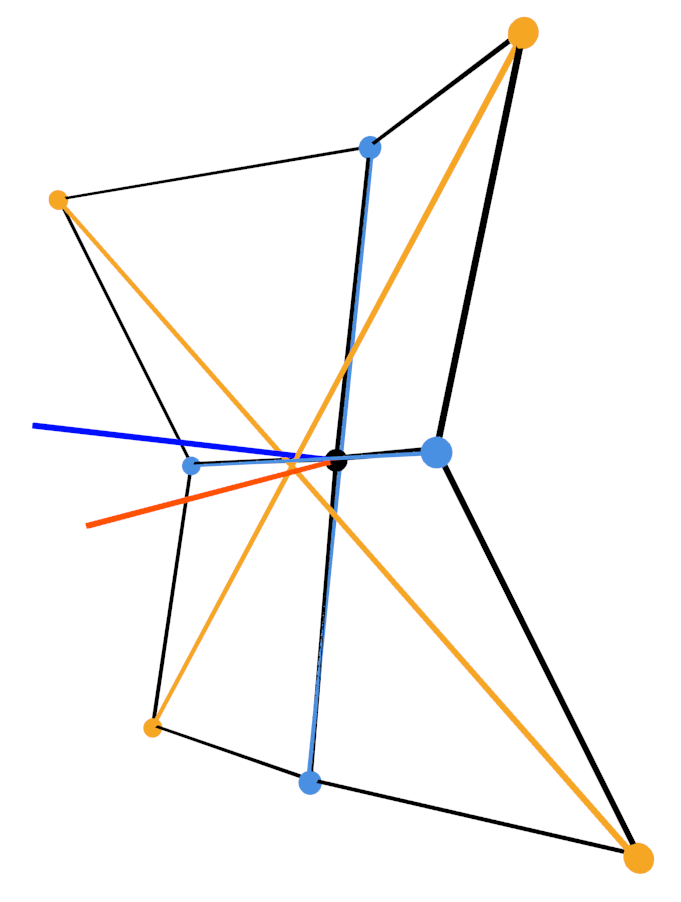
\includegraphics[width=0.6\textwidth]{chapter04/img/flexion-model-2-clipped.png}};
    \node at (4.4, 5.1) {$\mathbf{P_{i-1,j-1}}$};
    \node at (6.2, 5.5) {$\mathbf{P_{i,j-1}}$};
    \node at (8.5, 5.8) {$\mathbf{P_{i+1,j-1}}$};

    \node at (4.7, 2.9) {\scalebox{0.9}{$\mathbf{P_{i-1,j}}$}};
    \node at (6.2, 2.5) {$\mathbf{P_{i,j}}$};
    \node at (7.7, 3.0) {$\mathbf{P_{i+1,j}}$};

    \node at (5.0, 0.9) {$\mathbf{P_{i-1,j+1}}$};
    \node at (6.3, 0.4) {$\mathbf{P_{i,j+1}}$};
    \node at (9.2, 0.3) {$\mathbf{P_{i+1,j+1}}$};

    \node [plotdarkblue] at (4.6, 3.5) {$\vec{n_1}$};
    \node [plotdarkorange] at (4.8, 2.3) {$\vec{n_2}$};
\end{tikzpicture}

        }
        \caption{The estimated normals span an angle depending on the local shape of the surface measured by the depth sensors.}\label{fig:flexion_space}
    \end{subfigure}
    \caption[Schematic representation of the \gls{flexion-image} calculation]{\emph{Schematic representation of the \gls{flexion-image} calculation.} This figure demonstrates how flexed surfaces have different normals for diagonal and non-diagonal estimation. This difference is utilized as measure for flexion.}%
    \label{fig:flexion-image-scetched}
\end{figure}
Using the diagonal and vertical neighbouring points (blue) results a different normal than the diagonal neighbours (orange).
As Figure~\ref{fig:flexion_space} demonstrates, both normals span an angle.
\begin{equation}
\begin{aligned}
    \vec{n_1} &= \frac{\vec{P_{i,j-1}} - \vec{P_{i,j+1}}}{\lnorm{\vec{P_{i,j-1}} - \vec{P_{i,j+1}}}}
                \times \frac{\vec{P_{i-1,j}} - \vec{P_{i+1,j}}}{\lnorm{\vec{P_{i-1,j}} - \vec{P_{i+1,j}}}} \\
    \vec{n_2} &= \frac{\vec{P_{i-1,j-1}} - \vec{P_{i+1,j+1}}}{\lnorm{\vec{P_{i-1,j-1}} - \vec{P_{i+1,j+1}}}}
                \times \frac{\vec{P_{i-1,j+1}} - \vec{P_{i+1,j-1}}}{\lnorm{\vec{P_{i-1,j+1}} - \vec{P_{i+1,j-1}}}}
    \label{eq:flexion_normals}
\end{aligned}
\end{equation}
Note, that both normals $\vec{n_1}$ and $\vec{n_2}$ are not unit length, but only the direction vector between the neighbouring points of $\mathbf{P_{i,j}}$.
Finally, the Flexion $\mathcal{F}$ of point $\mathbf{P_{i,j}}$ is defined as
\begin{align}
    \mathcal{F} &= \abs{\vec{n_1} \cdotp \vec{n_2}}
\end{align}
Because $\lnorm{\vec{n_1}},\lnorm{\vec{n_2}} \in [0,1]$ the value of is bound to $\mathcal{F} \in [0, 1]$.
Creating the final image requires a linear scaling to the desired output image depth using Equation~\ref{eq:linear_scaling}.

Figure~\ref{fig:flexion_images} visualizes the \Gls{flexion-image} for the same camera positions as for the other feature images.
\begin{figure}[H]
    \begin{subfigure}[t]{0.32\textwidth}
        
\includegraphics[width=\linewidth]{chapter04/img/flexion-0001.png}
    \end{subfigure}
    \begin{subfigure}[t]{0.32\textwidth}
        
\includegraphics[width=\linewidth]{chapter04/img/flexion-0030.png}
    \end{subfigure}
    \begin{subfigure}[t]{0.32\textwidth}
        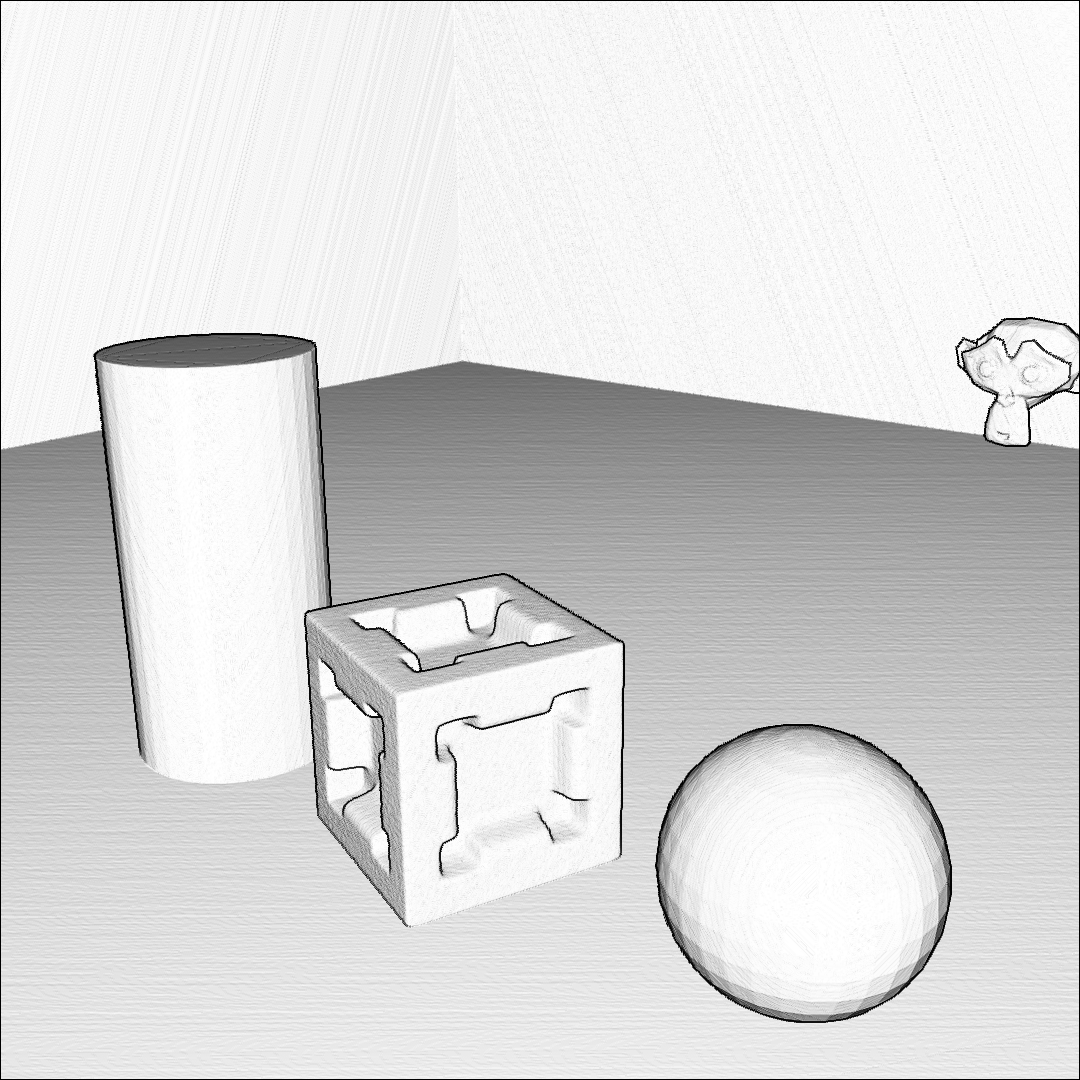
\includegraphics[width=\linewidth]{chapter04/img/flexion-0210.png}
    \end{subfigure}
    \caption[Characterstic look of a \gls{flexion-image}]{\emph{Characterstic look of a \gls{flexion-image}.} These figures demonstrate the characteristical look of the \Glspl{flexion-image}. Its appearence is very plastic and the shading effects give a good feel for depth. The conversion is rotation invariant.}\label{fig:flexion_images}
\end{figure}

\subsubsection*{Characteristics}

The \gls{flexion-image} is rotation invariant.
Rotation of either an object or the camera does not change the difference between the two normal approximations.
A flat surface has an almost constant shading, because the normal approximation results in the same vector directions.
Flat surfaces not perpendicular to the camera plane have non-constant shading with the brightness reduced the further the surface patch is appart from the camera center.
This effect is caused by the perspective transformation.
The length of the normal vectors reduces with the distance to the camera, because the diagonals gets smaller, as Figure~\ref{fig:flexion_angle_decrease} demonstrates.
\begin{figure}[H]
    

\tikzset{every picture/.style={line width=0.75pt}} %set default line width to 0.75pt        

\begin{tikzpicture}[x=0.75pt,y=0.75pt,yscale=-1,xscale=1]
%uncomment if require: \path (0,142); %set diagram left start at 0, and has height of 142

%Straight Lines [id:da6840514143989631] 
\draw [color={rgb, 255:red, 74; green, 144; blue, 226 }  ,draw opacity=1 ]   (366.4,69.04) -- (390.44,69.04) ;
%Straight Lines [id:da9689027017272559] 
\draw [color={rgb, 255:red, 74; green, 144; blue, 226 }  ,draw opacity=1 ]   (377.02,82.13) -- (377.02,55.88) ;
%Straight Lines [id:da8683032061954556] 
\draw [color={rgb, 255:red, 74; green, 144; blue, 226 }  ,draw opacity=1 ]   (451.65,69.04) -- (480.52,69.04) ;
%Straight Lines [id:da6934594327602702] 
\draw [color={rgb, 255:red, 74; green, 144; blue, 226 }  ,draw opacity=1 ]   (464.75,94.04) -- (465.02,44.04) ;
%Straight Lines [id:da7261021710957941] 
\draw [color={rgb, 255:red, 245; green, 166; blue, 35 }  ,draw opacity=1 ]   (480.5,42.14) -- (451.64,91.89) ;
%Straight Lines [id:da37992799055918147] 
\draw [color={rgb, 255:red, 245; green, 166; blue, 35 }  ,draw opacity=1 ]   (451.58,46) -- (480.5,95.1) ;
%Straight Lines [id:da15457235634391941] 
\draw [color={rgb, 255:red, 245; green, 166; blue, 35 }  ,draw opacity=1 ]   (389.38,54.43) -- (366.33,80.86) ;
%Straight Lines [id:da05878950535382432] 
\draw [color={rgb, 255:red, 245; green, 166; blue, 35 }  ,draw opacity=1 ]   (366.45,57.36) -- (390.5,83.43) ;
%Straight Lines [id:da045550454885305736] 
\draw [line width=3]    (80.9,107.5) -- (254.9,107.5) ;
%Shape: Circle [id:dp8549507101465224] 
\draw  [fill={rgb, 255:red, 0; green, 0; blue, 0 }  ,fill opacity=1 ] (16,39.5) .. controls (16,37.59) and (17.54,36.05) .. (19.45,36.05) .. controls (21.36,36.05) and (22.9,37.59) .. (22.9,39.5) .. controls (22.9,41.41) and (21.36,42.95) .. (19.45,42.95) .. controls (17.54,42.95) and (16,41.41) .. (16,39.5) -- cycle ;
%Straight Lines [id:da09684243305909856] 
\draw    (19.45,39.5) -- (94.9,106.5) ;
%Straight Lines [id:da4476141598512392] 
\draw    (19.45,39.5) -- (106.9,107.5) ;
%Straight Lines [id:da5555101325179832] 
\draw    (19.45,39.5) -- (204.9,107.5) ;
%Straight Lines [id:da06573307117836547] 
\draw    (19.45,39.5) -- (230.9,106.5) ;
%Shape: Circle [id:dp3195203497272404] 
\draw  [fill={rgb, 255:red, 0; green, 0; blue, 0 }  ,fill opacity=1 ] (274.67,69.08) .. controls (274.62,67.18) and (276.13,65.6) .. (278.04,65.55) .. controls (279.94,65.51) and (281.52,67.02) .. (281.57,68.92) .. controls (281.61,70.83) and (280.1,72.41) .. (278.2,72.45) .. controls (276.29,72.49) and (274.71,70.99) .. (274.67,69.08) -- cycle ;
%Straight Lines [id:da25083036265050096] 
\draw    (278.12,69) -- (496.79,97.97) ;
%Straight Lines [id:da6083860800665152] 
\draw    (278.12,69) -- (496.1,40.04) ;
%Shape: Rectangle [id:dp031034421219254926] 
\draw  [line width=3]  (301.4,9.5) -- (584.4,9.5) -- (584.4,126.5) -- (301.4,126.5) -- cycle ;
%Shape: Circle [id:dp2988386895287467] 
\draw  [fill={rgb, 255:red, 0; green, 0; blue, 0 }  ,fill opacity=1 ] (363.85,57.42) .. controls (363.81,55.99) and (364.95,54.8) .. (366.39,54.76) .. controls (367.82,54.73) and (369.01,55.87) .. (369.05,57.3) .. controls (369.08,58.74) and (367.94,59.93) .. (366.51,59.96) .. controls (365.07,60) and (363.88,58.86) .. (363.85,57.42) -- cycle ;
%Shape: Circle [id:dp49087747494377276] 
\draw  [fill={rgb, 255:red, 0; green, 0; blue, 0 }  ,fill opacity=1 ] (363.73,80.92) .. controls (363.69,79.48) and (364.83,78.29) .. (366.27,78.26) .. controls (367.7,78.23) and (368.89,79.36) .. (368.93,80.8) .. controls (368.96,82.23) and (367.82,83.42) .. (366.39,83.46) .. controls (364.95,83.49) and (363.76,82.35) .. (363.73,80.92) -- cycle ;
%Shape: Circle [id:dp3291682457892863] 
\draw  [fill={rgb, 255:red, 0; green, 0; blue, 0 }  ,fill opacity=1 ] (387.79,53.49) .. controls (387.75,52.06) and (388.89,50.87) .. (390.32,50.84) .. controls (391.76,50.8) and (392.95,51.94) .. (392.98,53.37) .. controls (393.02,54.81) and (391.88,56) .. (390.44,56.03) .. controls (389.01,56.07) and (387.82,54.93) .. (387.79,53.49) -- cycle ;
%Shape: Circle [id:dp598750640317177] 
\draw  [fill={rgb, 255:red, 0; green, 0; blue, 0 }  ,fill opacity=1 ] (387.91,83.49) .. controls (387.87,82.05) and (389.01,80.86) .. (390.44,80.83) .. controls (391.88,80.79) and (393.07,81.93) .. (393.1,83.37) .. controls (393.14,84.8) and (392,85.99) .. (390.56,86.03) .. controls (389.13,86.06) and (387.94,84.92) .. (387.91,83.49) -- cycle ;
%Shape: Circle [id:dp3156912690396848] 
\draw  [fill={rgb, 255:red, 0; green, 0; blue, 0 }  ,fill opacity=1 ] (449.04,91.95) .. controls (449.01,90.51) and (450.14,89.32) .. (451.58,89.29) .. controls (453.02,89.26) and (454.21,90.39) .. (454.24,91.83) .. controls (454.27,93.26) and (453.13,94.45) .. (451.7,94.49) .. controls (450.26,94.52) and (449.07,93.38) .. (449.04,91.95) -- cycle ;
%Shape: Circle [id:dp0381257221295519] 
\draw  [fill={rgb, 255:red, 0; green, 0; blue, 0 }  ,fill opacity=1 ] (448.99,46.21) .. controls (448.95,44.77) and (450.09,43.58) .. (451.53,43.55) .. controls (452.96,43.52) and (454.15,44.65) .. (454.18,46.09) .. controls (454.22,47.53) and (453.08,48.72) .. (451.65,48.75) .. controls (450.21,48.78) and (449.02,47.65) .. (448.99,46.21) -- cycle ;
%Shape: Circle [id:dp4047969379608699] 
\draw  [fill={rgb, 255:red, 0; green, 0; blue, 0 }  ,fill opacity=1 ] (477.91,42.2) .. controls (477.87,40.76) and (479.01,39.57) .. (480.44,39.54) .. controls (481.88,39.51) and (483.07,40.64) .. (483.1,42.08) .. controls (483.14,43.51) and (482,44.7) .. (480.56,44.74) .. controls (479.13,44.77) and (477.94,43.63) .. (477.91,42.2) -- cycle ;
%Shape: Circle [id:dp5781527725767942] 
\draw  [fill={rgb, 255:red, 0; green, 0; blue, 0 }  ,fill opacity=1 ] (477.91,95.16) .. controls (477.87,93.72) and (479.01,92.53) .. (480.44,92.5) .. controls (481.88,92.46) and (483.07,93.6) .. (483.1,95.04) .. controls (483.14,96.47) and (482,97.66) .. (480.56,97.69) .. controls (479.13,97.73) and (477.94,96.59) .. (477.91,95.16) -- cycle ;

% Text Node
\draw (12,50.05) node [anchor=north west][inner sep=0.75pt]   [align=left] {$\displaystyle \mathbf{C}$};
% Text Node
\draw (268,78.05) node [anchor=north west][inner sep=0.75pt]   [align=left] {$\displaystyle \mathbf{C}$};


\end{tikzpicture}

    \caption[Explanation of shading effect in \glspl{flexion-image}]{\emph{Explanation of shading effect in \glspl{flexion-image}.} The angle between the diagonals decreases with increasing distance from the camera center. This results in shorter normals.}\label{fig:flexion_angle_decrease}
\end{figure}
The origin is the nature of the cross product is maximal if both vectors are perpendicular.
\begin{equation*}
    \lnorm{\vec{v_1} \times \vec{v_2}} = \lnorm{\vec{v_1}} \lnorm{\vec{v_2}} \sin \angle(\vec{v_1}, \vec{v_2})
\end{equation*}
The lack of normalization in Equation~\ref{eq:flexion_normals} propagates this effect through to the scalar product.
\begin{equation*}
    \vec{v_1} \cdot \vec{v_2} = \lnorm{\vec{v_1}} \lnorm{\vec{v_2}} \cos \angle(\vec{v_1}, \vec{v_2})
\end{equation*}
This shading effect gives the \gls{flexion-image} its plastic look and helps to develop the feeling for the geometric constellations.

\subsubsection{Implementation Details}

All software developed during the thesis, including the analysis and supplementary code, are developed with rigor software engineering methods.
The library components have 100\,\% unit- and integrationtest line coverage.
Each final executable is heavily tested, too.
The overall line coverage for all project code is above $98\%$.
The implementation language is C++-17\cite{c++17} and all library depdencies use at least C++-11\cite{c++11}.
All code obeys to strong typing, design by contract\cite{meyer_ieee1992} and modern idioms of the C++ programming language\cite{stroustrup_cpppl2013}.
To uncover runtime problems potentially present in C++ through raw memory access, the LLVM Address-, Memory-, Thread- and Undefined-Behaviour-Sanitizers\cite{google_sanitizers} are run over all tests.
Additional static analysis is done by clang's thread-safety analysis\cite{clang_thread_safety}, clang static analyzer\cite{clang_static_analyzer} and clang-tidy\cite{babati2017static}.
All detected issues were immediately fixed during development.
The use of continuous integration\cite{fowler_ci2000} for the whole development cycle indicated defects within hours and ensured fast development of code with a low defect rate.

The implementation goal of the developed software is to serve as a correct reference implementation for the proposed feature images.
Therefore, no special action has been taken to improve latency or throughput of the computations.
Only simple measures for speedup, namely exploiting the embarrassingly parallel nature of the processing and compiler optimizations are employed.
Figure~\ref{fig:benchmarks} shows the results of micro benchmarks of the two promising feature images.
\begin{figure}
\centering
    \begin{subfigure}[b]{0.45\linewidth}
        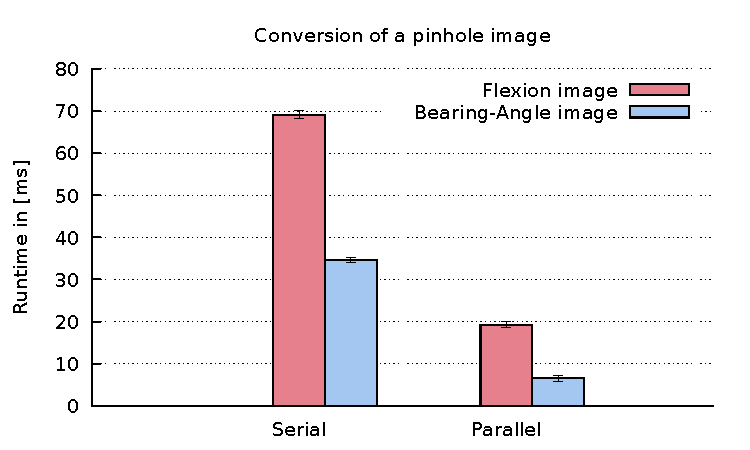
\includegraphics[width=\linewidth]{chapter06/results/benchmarks/pinhole_benchmarks.pdf}
    \end{subfigure}\quad
    \begin{subfigure}[b]{0.45\linewidth}
        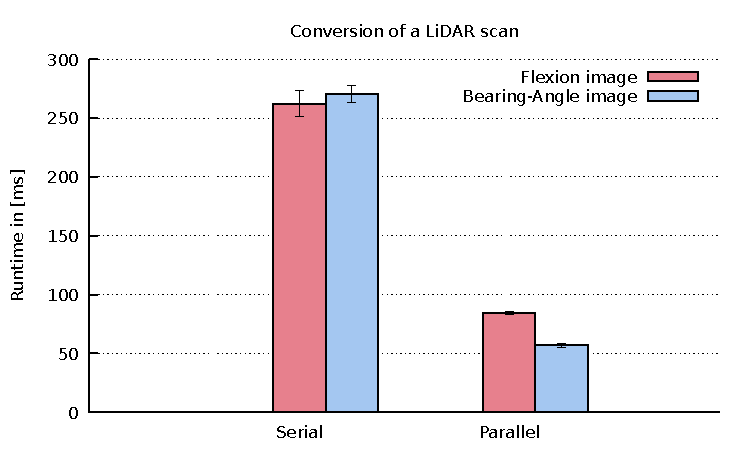
\includegraphics[width=\linewidth]{chapter06/results/benchmarks/laserscan_benchmarks.pdf}
    \end{subfigure}
    \caption[Benchmarks for Flexion and \gls{bearing-angle-image} conversions]{\emph{Benchmarks for Flexion and \gls{bearing-angle-image} conversions.} The benchmarks are run on an Intel i7-8550U with 1.8\,GHz base clock and 4 hyperthreaded cores. Each conversion is repeated 100 times for solid statistical data. The resolution of the pinhole image is 960$\times$540\,px and the \acrshort{LIDAR} scan is 3600$\times$800\,px big. The higher memory consumption of the \acrshort{LIDAR} scan results in a memory bound execution for the single threaded conversion.}\label{fig:benchmarks}
\end{figure}
Each of the feature image conversions is implemented as C++ library code working on OpenCV's\cite{opencv_library} \lstinline[basicstyle=\ttfamily]|cv::Mat| matrix type.
The conversion is generic in the sense, that any camera model implementing the forward and backward projection for pixel coordinates is suitable for the feature image conversion.
This genericity is achieved through the use of templates.
Type requirements are enforced with \lstinline[basicstyle=\ttfamily]|static_assert()| and concept-like\cite{c++concepts} requirement definitions.
One important type requirement ensures consistent use of coordinate systems with a special type that prohibits the code \texttt{\lstinline[language=C++,basicstyle=\footnotesize\ttfamily]|coordinate<float, frame::pixel> px = coordinate<float, frame::image>(0.5F, 0.25F);|} to compile.
All image access operations must adhere to the reference frame annotation and special transformations, like projections, are the only way to switch between coordinate systems.

Multiple library dependencies support the functionality of the project and shall be mentioned without a particular order.
The already mentioned OpenCV\cite{opencv_library} project provides functionality for image handling and processing. 
Required types and functionality for glue-code, parallelization and general programming utilize \emph{cli11}\cite{cli11}, \emph{rang}\cite{rang}, \emph{cpp-taskflow}\cite{Huang2019CppTaskflowFT}, \emph{fmt-lib}\cite{fmtlib}, \emph{GSL}\cite{gsl}, \emph{Eigen3}\cite{eigenweb} and \emph{Boost}\cite{boost}.
Functionality and performance testing are done with \emph{doctest}\cite{doctest} and \emph{libnonius}\cite{libnonius}.
Each used revision is documented in the code repository and differs between versions of the thesis code.


\subsection{Feature Detection and Description}\label{sec:feature_algorithms}

After preprocessing and image conversion, the final processing step of the range data is the feature detection and description.
This thesis analyzes \acrshort{sift}\cite{lowe_ijcv04}, \acrshort{surf}\cite{bay_eccv06}, \acrshort{orb}\cite{rublee_iccv11} and \acrshort{akaze}\cite{alcantarilla_bmva13}.
Although each keypoint detector and descriptor is designed with gray-scale images in mind, they are optimized for classical camera images that provide more texture than the converted feature images.
Key to all algorithms is the search for salient regions in the image that can be consistently detected from different viewpoints and changing environmental conditions.
The detector performance is critical to apply classical image registration approaches to the converted feature images.
The following sections introduce the algorithms briefly and mentions key aspects of their functionality.
Details and foundational concepts are out of scope and the original publications are highly recommended for further comprehension.

\subsubsection{\acrshort{sift} (\acrlong{sift})}

Introduced by Lowe\cite{lowe_iccv99,lowe_ijcv04}, \acrshort{sift} is an established feature detection algorithm.
The design goal of the algorithm is to detect keypoints that are invariant with respect to scale and rotation.
Robustness against noise, change in illumination and affine transformations is additionally considered.
\acrshort{sift}'s design influenced the design decisions of the other presented algorithms heavily.

The input image is processed in a hierarchical pyramid of downscaled versions of the image, called octaves.
On each octave a Gaussian filter is applied consecutivly with increased standard deviation on each run.
The difference between two consecutive blurred images is computed, the so called \acrlong{DoG} (\acrshort{DoG}) forming an approximation of the Laplacion of the image.
Lindeberg's\cite{lindeberg_ijcv98} work on scale space and automatic scale selection gives a theoretical introduction why this process gives a good way to select the scale of features.
The underlying principle exploits that fine structures dissolve at bigger scales.
This process is related to the diffusion equation that is strongly tied to the Laplacian of the image.
Keypoint candidates are local extrema in these \acrshort{DoG}s.
Each candidate is filtered by a contrast threshold, its accurate position is determined using a local spline interpolation and its scale is assigned based on the octave and blurring factor.
Edge-like responses are filtered out based on an estimate of the ratio between the principal curvatures.
Highly skewed curvatures indicate an edge.

Every keypoint candidate gets one or more orientations assigned.
These are computed by storing the gradients of a local neighbourhood to the keypoints in the octave matching the keypoints scale in an orientation histogram.
Each peak in this histogram reflects a dominant direction of gradients in the local neighbourhood and the corresponding angle is used as the orientation of the keypoint.
According to Lowe\cite{lowe_ijcv04}, about 15\% of keypoints have multiple peaks and get multiple orientations assigned.
The orientation is used to rotate the local neighbourhood of the keypoint to compute the descriptor consistently.

The image gradients direction and magnitude are computed for each pixel in a local environment, first weighted by a Gaussian to magnify the influence of close pixels and then binned into orientation histograms.
Each histogram reflects a fraction of the sampling grid.
A 16$\times$16 grid around the keypoint that is stored to 4$\times$4 histograms with 8 bins for the orientations results in a vector of 128 elements in the descriptor.
These dimensions can be adjusted, but the 128 element descriptor is most common.
Finally, the histograms are normalized to increase robustness against illumination changes.
The Euclidean distance of the descriptor vectors is the most common similarity measure.
Arandjelović and Zisserman\cite{arandjelovic_2012} introduced RootSIFT using the Hellinger distance\cite{hellinger_1909} as better measure for similarity of histograms.

\subsubsection{\acrshort{surf} (\acrlong{surf})}

Bay et al. introduced \acrshort{surf}\cite{bay_eccv06} to achieve similar detector and descriptor performance as \acrshort{sift} but at a lower computational cost.
\acrshort{surf} utilizes integral images\cite{viola_cvpr01}.
Each pixel's value is the sum of all pixels in the rectangle formed by the origin and the pixel itself.
This representation reduces computational complexity.

The underlying principal of scale space and extrema detection derives from the same principles as for \acrshort{sift} but undergoes simplification.
The Gaussian convolution is approximated with a box filter that approximate a second order Gaussian derivative and is related to the Hessian matrix.
Instead of building a pyramid of images at different scales, the filter itself is scaled up successively.
Maxima undergo a non-maximum suppression at different scales.
The maximum of the Hessian determinant for the detected pixel is interpolated in image scale and space.
The determinants value is the keypoint's response.

Orientation assignment of \acrshort{surf} can be skipped for scenarios that do not involve camera rotation.
The rotation is derived from the Haar wavelets\cite{haar_1911} response in $x$ and $y$ direction in the local neighbourhood.
The descriptor itself is constructed from a 4$\times$4 grid structure of sample points around the detected keypoint.
Again, the Haar wavelets response in $x$ and $y$ direction are used to derive the elements of the descriptor.

\subsubsection{\acrshort{orb} (\acrlong{orb})}

\acrshort{orb}\cite{rublee_iccv11} combines the \acrshort{fast}\cite{rosten_eccv06} (\acrlong{fast}) feature detector and \acrshort{brief}\cite{calonder_eccv10} (\acrlong{brief}) descriptor with additional improvements to both algorithms.
The design goal is to achieve similar matching performance to \acrshort{sift} and \acrshort{surf} but to be computationally cheaper to make usage in embedded devices feasable.

The \acrshort{fast} detector evaluates a each pixel by testing the brightness of 16~pixels on a circle around the corner.
If there are enough consecutive pixels brighter or darker than the center with a certain threshold, the pixel is accepted as corner.
This approach results in a decision tree.
The optimal traversal of this tree is learned by observing real world execution of the algorithm on predefined traversal.
\acrshort{orb} detects keypoints with \acrshort{fast}, filters edge results with the Harris corner detector\cite{harris_1988} and assigns scale using image pyramids.
The orientation of the keypoint is computed with the \emph{intensity centroid}\cite{rosin_cviu99}.

Each keypoint's descriptor uses a rotated version of \acrshort{brief}.
\acrshort{brief} is a binary descriptor built from a set of binary intensity tests of consecutive pixels around the keypoint.
The more recent publications, like \acrshort{brief}, \acrshort{orb} and \acrshort{mldb}, employ binary descriptors for their fast matching speed.
The distance of binary descriptors can be computed with the Hamming distance that reduces to \emph{XOR} instructions on machine level.
Ziegler et al.\cite{ziegler_anips2012} provide a theoretical analysis of \acrshort{brief} and its sibblings and show, that those are hashing schemes of Kendall's $\tau$ metric\cite{kendall_1938}.

\subsubsection{\acrshort{akaze}}

\acrshort{kaze}'s\cite{alcantarilla_eccv12} (\acrlong{kaze}) and \acrshort{akaze}'s\cite{alcantarilla_bmva13} (\acrlong{akaze}) approaches are similar to \acrshort{sift}'s.
Again, the diffusion of the brightness is the starting point for scale space analysis.
\acrshort{kaze} applies non-linear diffusion filtering with a special computational scheme, that makes it feasable to solve the diffusion in real time.
The difference to the Gaussian blurring is the preservation of edges.
The Gaussian blurs the whole image, reducing the signal crispness at higher scales.
Contrary, the non-linear diffusion preserves edges over higher scales.
After non-maximum suppression, the determinant of the Hessian is computed and the interpolation of the maximum on different scales yields the position of the keypoint.
The orientation of the keypoint is, similar to \acrshort{sift}, the dominant direction of the derivatives in the local neighbourhood of the keypoint.

The descriptor is \acrshort{mldb} (\acrlong{mldb}), which is based on \acrshort{ldb}\cite{yang_ismar12} (\acrlong{ldb}).
It works very similar to \acrshort{brief}.
But instead of comparing intensities of sampled pixel, it compares the average intensities of sampled areas around the keypoint.
The orientation of the keypoint is taken into account when sampling the areas.

\newpage

\section{Experiments}

The experiments evaluate the performance of the \gls{bearing-angle} and \glspl{flexion-image} for a variety of sensors, datasets and processing setups.
They demonstrate both success and failure under certain circumstances.
Both qualitative and quantitative aspects are considered in the evaluation.
Section~\ref{sec:results} presents and discusses these results.

\subsection{Datasets}

\subsubsection{Synthetic}\label{sec:dataset_synthetic}

The first dataset is a manually created scene in Blender\cite{blender} demonstrating the principle effects of rotation and translation on the conversion results.
Both rotation and translation are done in isolation as well combined.
The scene consists of a sphere, a cylinder, a cube-like object with additional edges of different smootheness and a complex monkey head in a room (Figure~\ref{fig:blender_scene}).
The camera movement is rendered as an animation and the depth buffer of each frame is extracted and used as depth image.
The camera matrix is calculated from the rendering settings and its parameters are provided in Table~\ref{tab:blender_intrinsic}.
The total animation consists of 211 images and no noise is applied to the depth image (example images in Appendix~\ref{sec:synthetic_conversions}).
\begin{figure}[H]
\CenterFloatBoxes%
\begin{floatrow}
    \btabbox{%
    \renewcommand{\arraystretch}{1.2}%
    \setlength{\tabcolsep}{1em}%
    \begin{tabular}{rc}
    \toprule
    \textbf{Parameter} & \textbf{Blender Camera} \\
    \midrule
    Principle  & render/pinhole \\
    Resolution & 1080 $\times$ 1080\,px \\
    $f_x$, $f_y$ & 2220.0, 2220.0 \\
    $c_x$, $c_y$ &  540.0, 540.0 \\
    \bottomrule
    \end{tabular}}
    {\caption{Blender camera intrinsic}\label{tab:blender_intrinsic}}%
    \ffigbox{%
    
\includegraphics[width=0.5\linewidth]{chapter05/img/blender/blender_render01.png}%
    
\includegraphics[width=0.5\linewidth]{chapter05/img/blender/depth_image_scene0005.png}%
    }
    {\caption{One frame as normal synthetic and depth image.}\label{fig:blender_scene}}
\end{floatrow}
\end{figure}

\subsubsection{Mine}

One real-world dataset is obtained with a mobile robot using a Kinectv2 in an underground mining environment, the \emph{Lehrpfad} of the Reiche Zeche, the education and research mine of the TU Bergakademie Freiberg.
The route has been previously reconstructed with \gls{sfm} using color images.
Due to the global optimization in the \gls{sfm} pipeline not preserving the proper scale for the depth images, the translations do not match the measured distances of the depth sensor.
The preexisting poses are used as initial pose for ICP refinement.
\emph{Mine} is the biggest tested dataset with 734 frames and has the biggest variation in the visible structures (example images in Appendix~\ref{sec:lehrpfad_conversions}).
It is a challenging dataset with high amount of noise, many missing depth values and differing data quality over the whole set of images.
\begin{figure}[H]
\CenterFloatBoxes%
\begin{floatrow}
    \btabbox{%
    \renewcommand{\arraystretch}{1.2}%
    \setlength{\tabcolsep}{1em}%
    \begin{tabular}{rc}
    \toprule
    \textbf{Parameter} & \textbf{Kinectv2} \\
    \midrule
    Principle  & pinhole \\
    Resolution & 960 $\times$ 540\,px \\
    $f_x$, $f_y$ & 519.23, 522.23 \\
    $c_x$, $c_y$ &  479.46, 272.74 \\
    \bottomrule
    \end{tabular}}
    {\caption{Mine Kinectv2 intrinsic.}\label{tab:lehrpfad_intrinsic}}%
    \ffigbox{%
    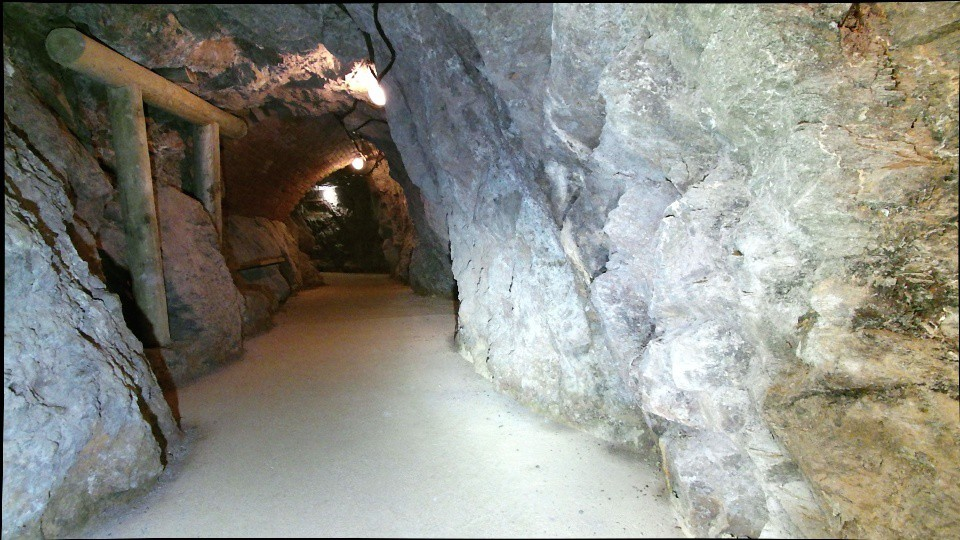
\includegraphics[width=0.5\linewidth]{chapter05/img/lehrpfad/color0000.jpg}%
    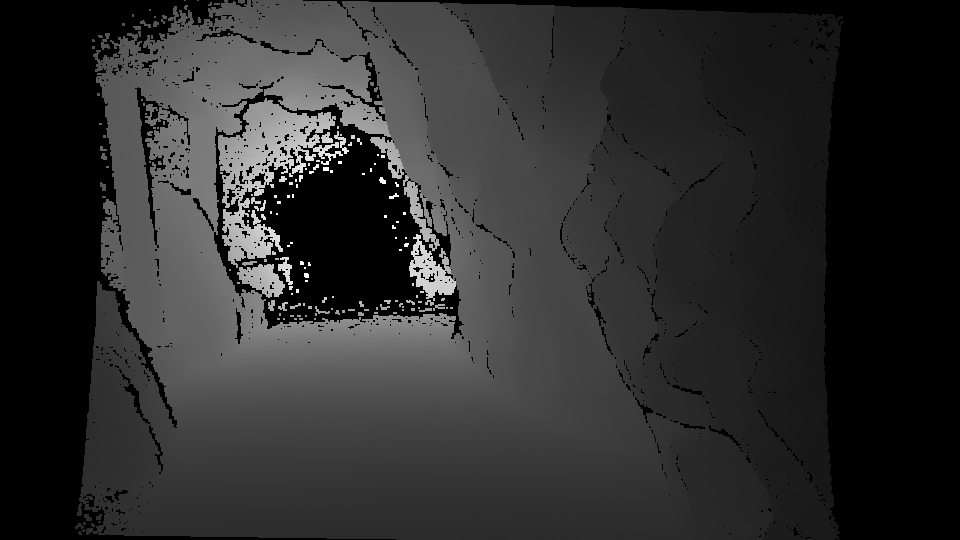
\includegraphics[width=0.5\linewidth]{chapter05/img/lehrpfad/depth-scaled-0000.png}\\
    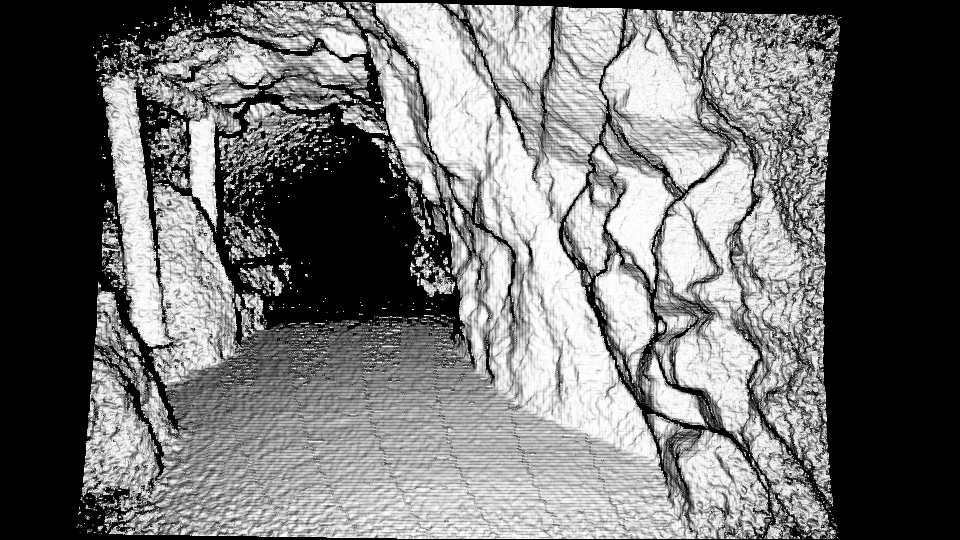
\includegraphics[width=0.5\linewidth]{chapter05/img/lehrpfad/flexion-0000.png}%
    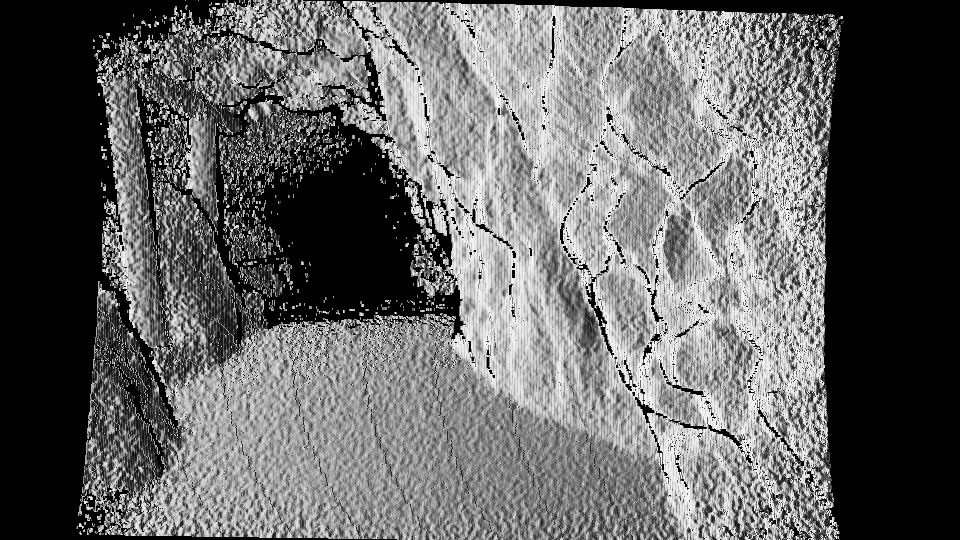
\includegraphics[width=0.5\linewidth]{chapter05/img/lehrpfad/bearing-0000.png}%
    }
    {\caption{Images of the \emph{Mine} dataset.}\label{fig:lehrpfad_data}}
\end{floatrow}
\end{figure}

\subsubsection{Office}

The second Kinectv2 dataset is taken in an office with many smaller elements, wires and other manmade objects.
It contains 57 images composed of translation and rotation of the depth sensor (example images in Appendix~\ref{sec:office_conversions}).
No trajectory reconstruction other than the ICP is used for the relative poses.
It contains similar measurement errors as the Mine dataset, but has more distinctive shapes and better overall conditions for the depth sensor.
\begin{figure}[H]
\CenterFloatBoxes%
\begin{floatrow}
    \btabbox{%
    \renewcommand{\arraystretch}{1.2}%
    \setlength{\tabcolsep}{1em}%
    \begin{tabular}{rc}
    \toprule
    \textbf{Parameter} & \textbf{Kinectv2} \\
    \midrule
    Principle  & pinhole \\
    Resolution & 960 $\times$ 540\,px \\
    $f_x$, $f_y$ & 519.23, 522.23 \\
    $c_x$, $c_y$ &  479.46, 272.74 \\
    \bottomrule
    \end{tabular}}
    {\caption{Office Kinectv2 intrinsic.}\label{tab:office_intrinsic}}%
    \ffigbox{%
    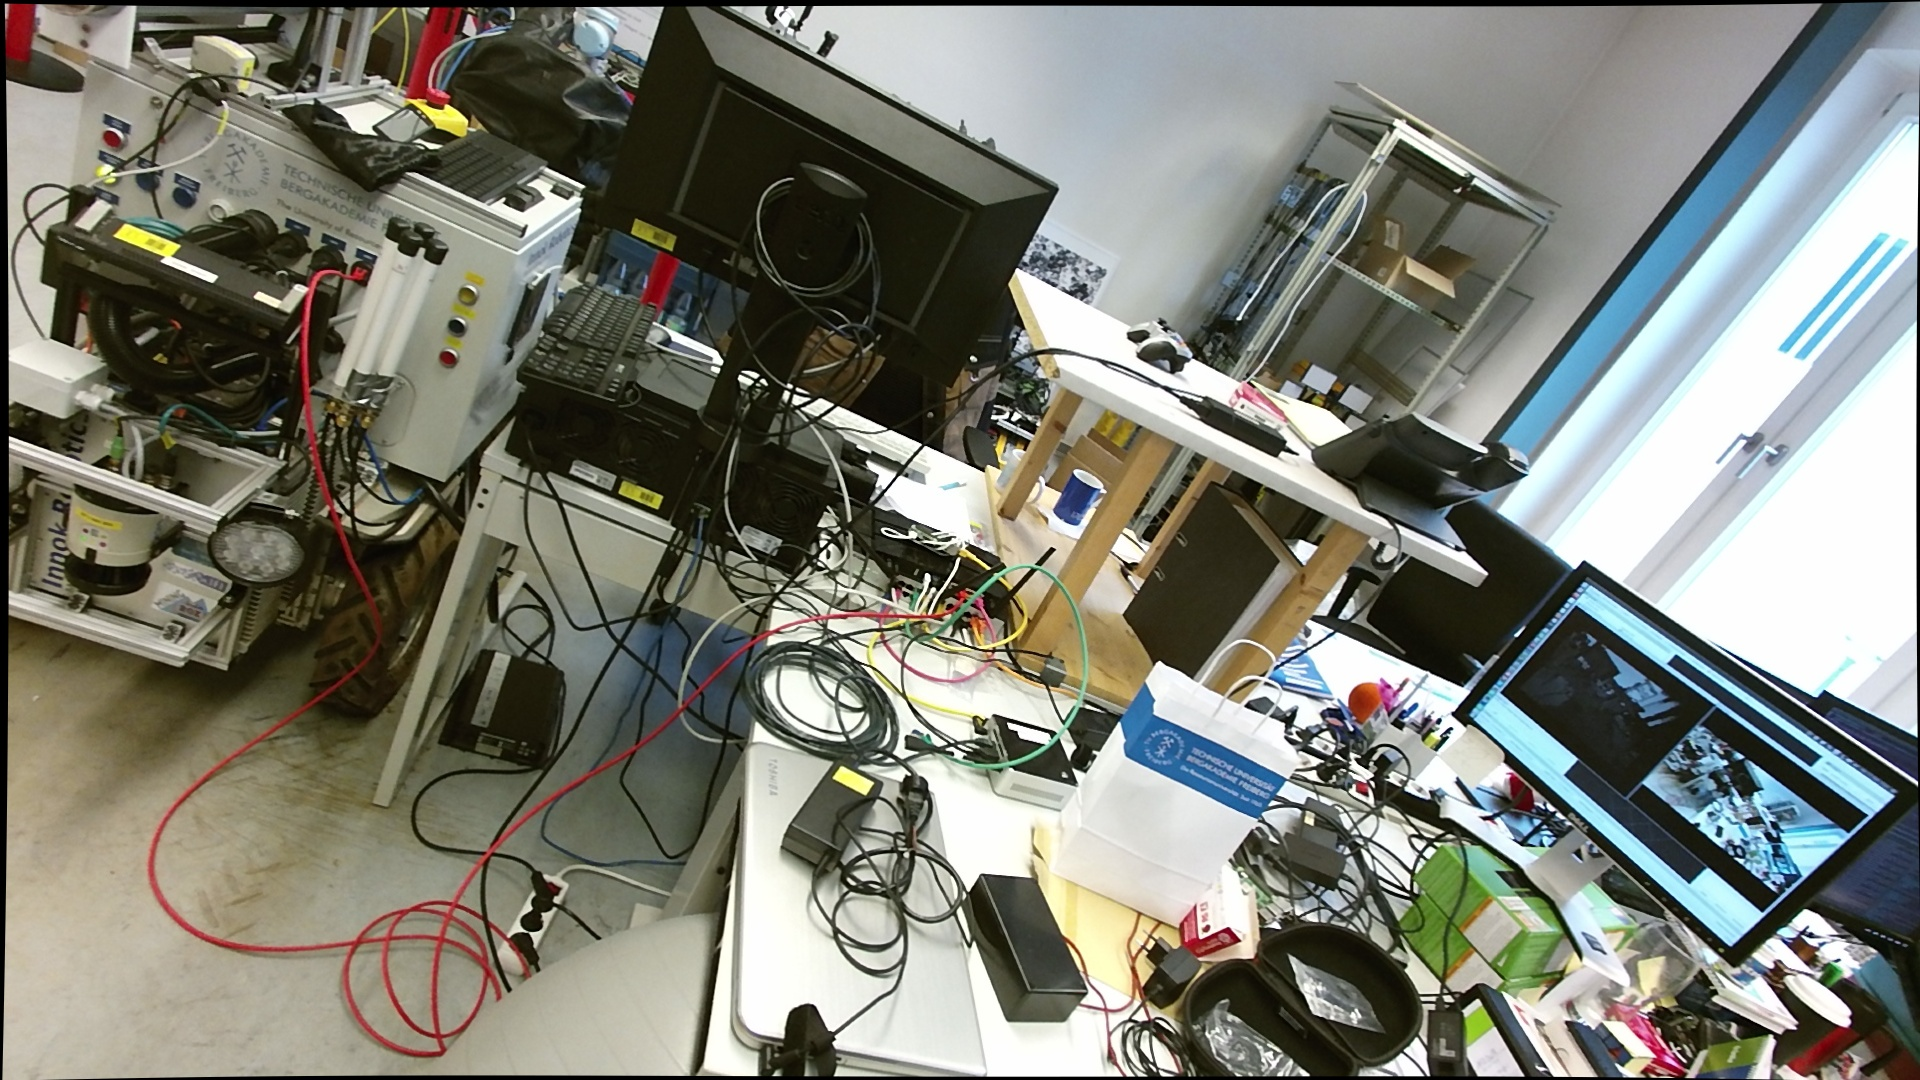
\includegraphics[width=0.5\linewidth]{chapter05/img/office/color_0024.jpg}%
    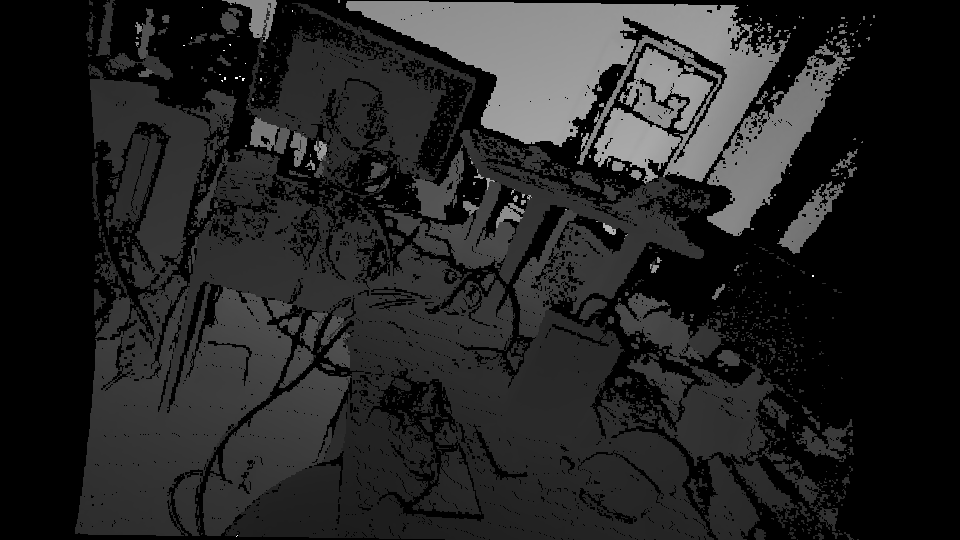
\includegraphics[width=0.5\linewidth]{chapter05/img/office/depth_scaled_0024.png}\\
    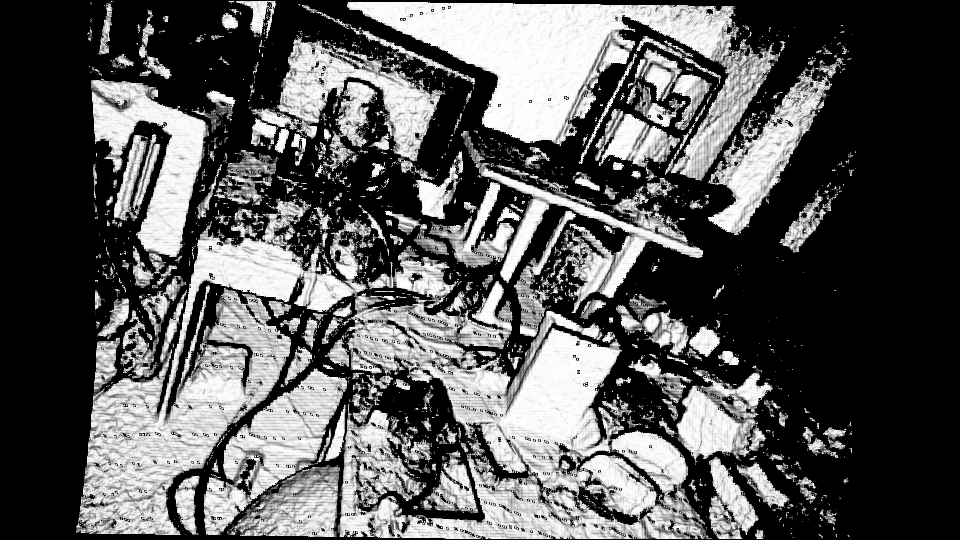
\includegraphics[width=0.5\linewidth]{chapter05/img/office/flexion_0024.png}%
    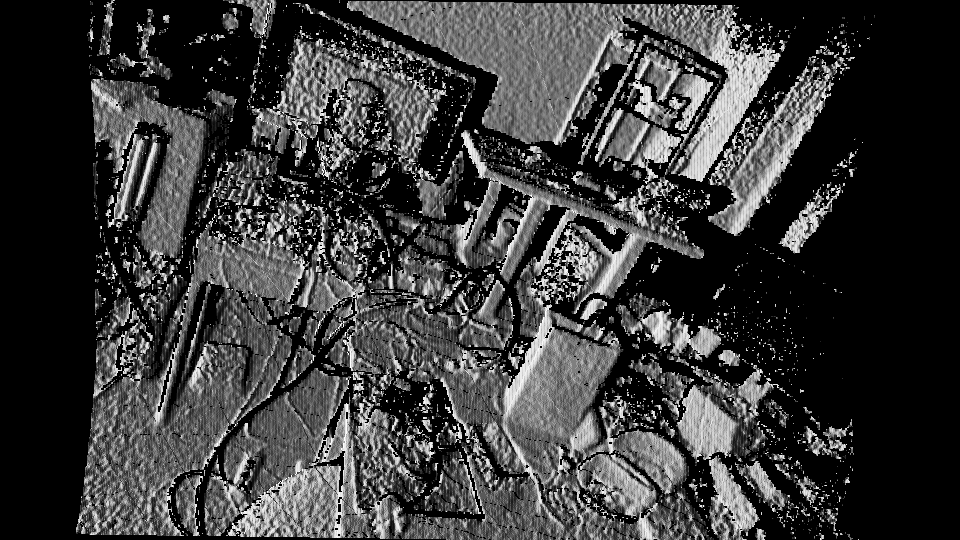
\includegraphics[width=0.5\linewidth]{chapter05/img/office/bearing_0024.png}%
    }
    {\caption{Images of the \emph{Office} dataset.}\label{fig:office_data}}
\end{floatrow}
\end{figure}

\subsubsection{Laserscan}

Full \acrshort{LIDAR} scans are taken as part of classical mine surveying in the Reiche Zeche.
The scans were done in the section \emph{Wilhelm-Stehender-Süd} of the mine.
These scans are examined for the conversions, too.
Because they were done with classical artificial marker based registration in mind, the overlap between those scans is minimal.
This unfortunatly means, that a direct matching between scans would be meaningless.
The distribution and characteristics of the extracted features is analyzed, though.
From the raw dataset only 6 scans are selected, because each scan had a slightly different resolution and aspect ratio (example scans in Appendix~\ref{sec:laserscan_conversions}).
The selected scans were manually processed to have a common resolution and aspect ratio.
\begin{figure}[H]
\CenterFloatBoxes%
\begin{floatrow}
    \btabbox{%
    \renewcommand{\arraystretch}{1.2}%
    \setlength{\tabcolsep}{1em}%
    \begin{tabular}{rc}
    \toprule
    \textbf{Parameter} & \textbf{Riegl Z300} \\
    \midrule
    Principle  & equirectangular \\
    Resolution & 3600 $\times$ 800\,px \\
    $\theta_{min}$, $\theta_{max}$ & \shortstack{0.87, 2.27 \\ (49.85\degree, 130.06\degree)} \\
    \bottomrule
    \end{tabular}}
    {\caption{Riegl Z300 \acrshort{LIDAR} intrinsic.}\label{tab:scan_intrinsic}}%
    \ffigbox{%
    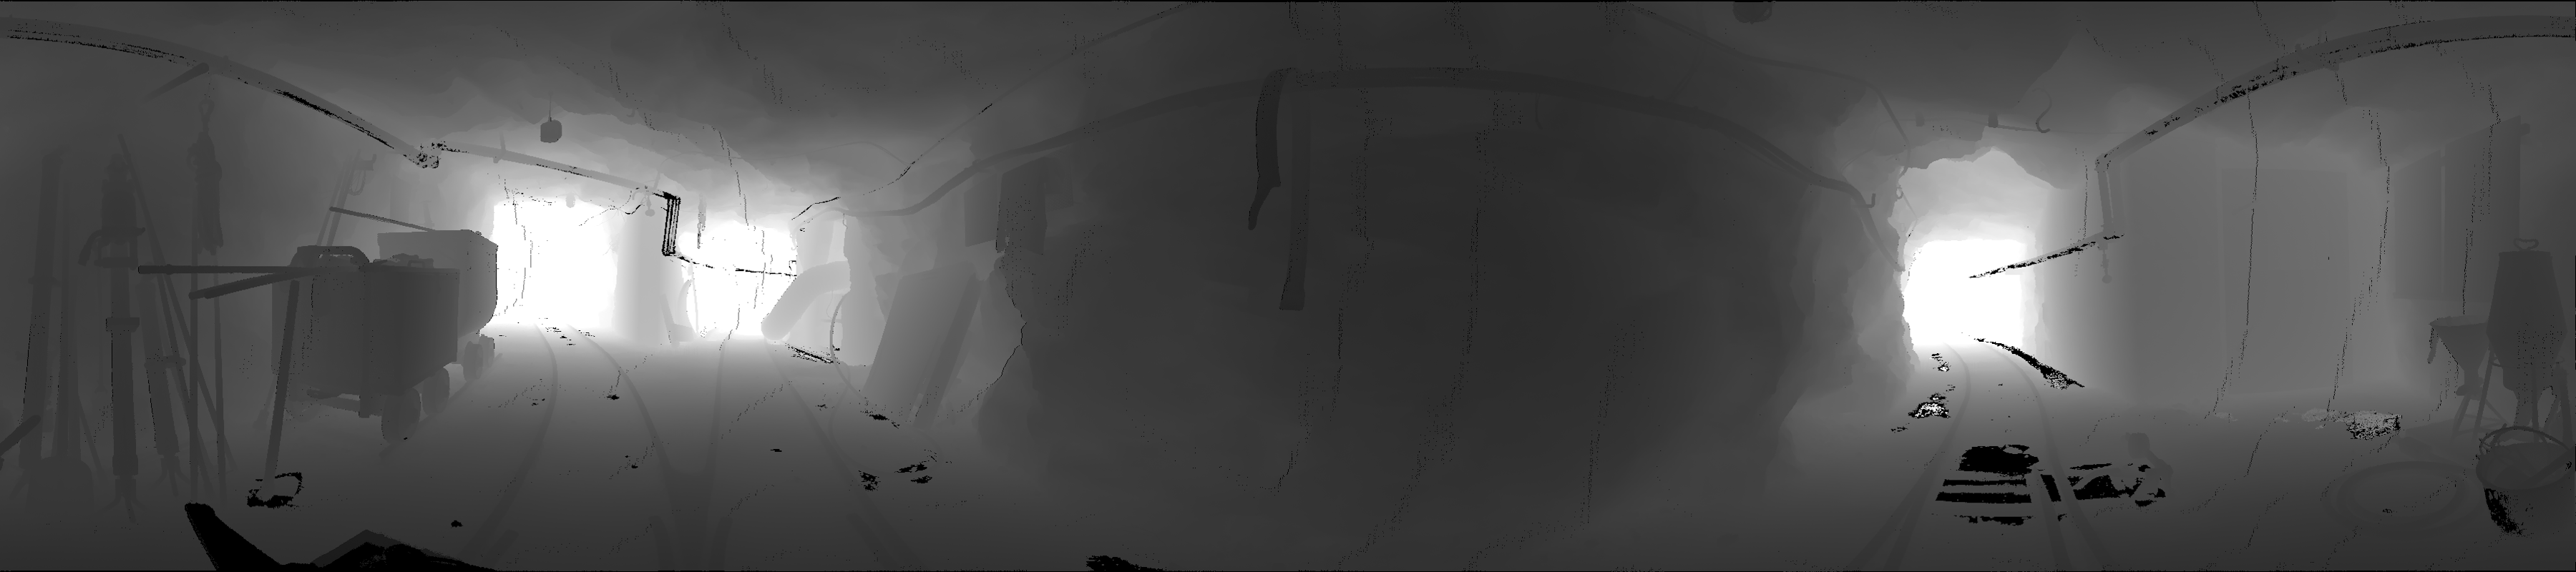
\includegraphics[width=1\linewidth]{chapter05/img/scans/range-0001.png}\\
    
\includegraphics[width=1\linewidth]{chapter05/img/scans/flexion-0001.png}\\
    \includegraphics[width=1\linewidth]{chapter05/img/scans/bearing-0001.png}%
    }
    {\caption{The raw \acrshort{LIDAR} scans and their conversions.}\label{fig:scans}}
\end{floatrow}
\end{figure}

\begin{table}[H]
    {\renewcommand{\arraystretch}{1.3}%
    \setlength{\tabcolsep}{0.3em}%
    \begin{tabular}{ccccc}
    \toprule
    \null & \textbf{Synthetic} & \textbf{Mine} & \textbf{Office} & \textbf{Laserscan} \\
    \midrule
    \textbf{Camera Model} & pinhole & pinhole & pinhole & equirectangular \\
    \textbf{Number Images} & 211 & 734 & 57 & 6 \\
    \textbf{Distribution} & \ding{52} & \ding{52} & \ding{52} & \ding{52} \\
    \textbf{Keypoint Characteristics} & \ding{52} & \ding{52} & \ding{52} & \ding{52} \\
    \textbf{Matching Performance} & \ding{52} & \ding{52} & \ding{52} & \ding{56} \\
    \bottomrule
    \end{tabular}
    }
    \caption{An overview of all datasets and aspects of them were analyzed.}
\end{table}

\subsubsection{Synthetic City Scene Odometry}

The datasets presented before evaluate the feature algorithms and show their potential and performance.
To demonstrate, that the results are applicable in other scenarios, the most promising algorithms are used to compute a visual odometry.
A synthetic city dataset (Section~\ref{sec:odometry_images}), developed by Zhang et al.\cite{zhang_icra2016}, that provides a groundthruth trajectory serves as test.
The in-house visual odometry implementation, based on Singh's\cite{singh_report2015} work, is very basic with the following four steps.
First, the features are detected and their descriptors extracted.
The descriptors are matched.
The essential matrix is computed using RANSAC and the consensus pose is used as relative pose.
Each feature algorithm is executed with its default configuration.
Both conditions imply that the result is not optimal and further optimizations would improve it further.

\subsection{Metrics}

To determine the performance of the feature-based approach, the matching of keypoints is framed in terms of a binary classifier.
For a keypoint correspondence between two images, the classification task is to determine if those keypoints correspond to the same point in the real world or not.
The correspondence is computed based on the relative pose of consecutive images and only two consecutive images are analyzed.
The following subsections describe each component of this evaluation pipeline in more detail.

\subsubsection{Ground truth Poses}

The dataset \emph{Mine} provides ground truth poses from a prior \gls{sfm} reconstruction.
Due to the global optimization of the \gls{sfm} algorithm, these poses do not match with the depth values of the depth images.
The other datasets do not contain a precomputed pose.
Therefore, each pose is computed and refined with an ICP algorithm, namely OpenCV's \texttt{FASTICPOdometry}\cite{opencv_library} that is based on the KinectFusion\cite{newcombe_ismar2011} work.
This relative pose serves as foundation of the evaluation and is assumed to be correct within small tolerance.
The accuracy assumption of the \texttt{FASTICPOdometry} poses is tested by manual inspection of the backprojection of obviously related keypoints and the results showed no systematic erroneous poses.

\subsubsection{Backprojection and Distance Threshold}

In two consecutive images, all keypoints are extracted with the chosen algorithm and settings.
Each keypoint of the first image $I_1$ is projected to the unit sphere, e.g. with Equation~\ref{eq:pinhole_backward}, multiplied with the range value of the corresponding pixel and the resulting camera coordinate transformed to the second camera coordinate system (Equation~\ref{eq:homogeneous_matrix}).
Projecting the keypoint into the second camera with the matching forward projection (e.g. Equation~\ref{eq:pinhole_forward}) finalizes the procedure, demonstrated in Figure~\ref{fig:keypoint_projection}.
This results in two sets of keypoints in the second image $I_2$, the keypoints detected in this frame and the keypoints detected in the previous frame, seen from this frame's pose.
Assuming a correct relative pose, the corresponding keypoints have a small pixel distance between each other.
\emph{Small} is a relative value and the chosen threshold in the experiments is 2\,px.
This approach can only result in a proper analysis for a sparse distribution of keypoints that actually correspond to image structure and requires small changes in pose.
When the pose difference is big, it can happen that keypoints get projected to the same position as some other valid keypoint without referencing the same world point.
Too many points create ambiguity with respect to the backprojection tolerance.
\begin{figure}[b!]
    

\tikzset{every picture/.style={line width=0.75pt}} %set default line width to 0.75pt        

\begin{tikzpicture}[x=0.75pt,y=0.75pt,yscale=-1,xscale=1]
%uncomment if require: \path (0,229); %set diagram left start at 0, and has height of 229

%Shape: Rectangle [id:dp6786998235335104] 
\draw   (21.88,21.67) -- (253.33,21.67) -- (253.33,189.54) -- (21.88,189.54) -- cycle ;
%Shape: Polygon [id:ds4691410097865978] 
\draw  [fill={rgb, 255:red, 0; green, 0; blue, 0 }  ,fill opacity=1 ] (127.01,83.56) -- (164.31,128.49) -- (111.75,109) -- (64.27,123.41) -- (60.88,86.1) -- cycle ;
%Shape: Circle [id:dp07615520367165762] 
\draw  [draw opacity=0][fill={rgb, 255:red, 74; green, 144; blue, 226 }  ,fill opacity=1 ] (160.08,128.49) .. controls (160.08,126.15) and (161.97,124.26) .. (164.31,124.26) .. controls (166.66,124.26) and (168.55,126.15) .. (168.55,128.49) .. controls (168.55,130.84) and (166.66,132.73) .. (164.31,132.73) .. controls (161.97,132.73) and (160.08,130.84) .. (160.08,128.49) -- cycle ;
%Shape: Ellipse [id:dp6448504150595761] 
\draw  [draw opacity=0][fill={rgb, 255:red, 74; green, 144; blue, 226 }  ,fill opacity=1 ] (122.77,83.56) .. controls (122.77,81.22) and (124.67,79.32) .. (127.01,79.32) .. controls (129.35,79.32) and (131.25,81.22) .. (131.25,83.56) .. controls (131.25,85.9) and (129.35,87.8) .. (127.01,87.8) .. controls (124.67,87.8) and (122.77,85.9) .. (122.77,83.56) -- cycle ;
%Shape: Ellipse [id:dp7051810352399743] 
\draw  [draw opacity=0][fill={rgb, 255:red, 74; green, 144; blue, 226 }  ,fill opacity=1 ] (107.51,109) .. controls (107.51,106.65) and (109.41,104.76) .. (111.75,104.76) .. controls (114.09,104.76) and (115.99,106.65) .. (115.99,109) .. controls (115.99,111.34) and (114.09,113.23) .. (111.75,113.23) .. controls (109.41,113.23) and (107.51,111.34) .. (107.51,109) -- cycle ;
%Shape: Ellipse [id:dp9159085548976601] 
\draw  [draw opacity=0][fill={rgb, 255:red, 74; green, 144; blue, 226 }  ,fill opacity=1 ] (60.04,123.41) .. controls (60.04,121.07) and (61.93,119.17) .. (64.27,119.17) .. controls (66.62,119.17) and (68.51,121.07) .. (68.51,123.41) .. controls (68.51,125.75) and (66.62,127.65) .. (64.27,127.65) .. controls (61.93,127.65) and (60.04,125.75) .. (60.04,123.41) -- cycle ;
%Shape: Ellipse [id:dp49160949647303864] 
\draw  [draw opacity=0][fill={rgb, 255:red, 74; green, 144; blue, 226 }  ,fill opacity=1 ] (56.64,86.1) .. controls (56.64,83.76) and (58.54,81.87) .. (60.88,81.87) .. controls (63.22,81.87) and (65.12,83.76) .. (65.12,86.1) .. controls (65.12,88.45) and (63.22,90.34) .. (60.88,90.34) .. controls (58.54,90.34) and (56.64,88.45) .. (56.64,86.1) -- cycle ;
%Shape: Polygon [id:ds13360398877823854] 
\draw  [fill={rgb, 255:red, 0; green, 0; blue, 0 }  ,fill opacity=1 ] (201.67,91.58) -- (232.66,121.16) -- (210.12,157.78) -- (191.81,131.01) -- cycle ;
%Shape: Ellipse [id:dp8706054475141728] 
\draw  [draw opacity=0][fill={rgb, 255:red, 74; green, 144; blue, 226 }  ,fill opacity=1 ] (205.89,157.78) .. controls (205.89,155.43) and (207.78,153.54) .. (210.12,153.54) .. controls (212.47,153.54) and (214.36,155.43) .. (214.36,157.78) .. controls (214.36,160.12) and (212.47,162.01) .. (210.12,162.01) .. controls (207.78,162.01) and (205.89,160.12) .. (205.89,157.78) -- cycle ;
%Shape: Circle [id:dp6356920604931994] 
\draw  [draw opacity=0][fill={rgb, 255:red, 74; green, 144; blue, 226 }  ,fill opacity=1 ] (228.42,121.16) .. controls (228.42,118.81) and (230.32,116.92) .. (232.66,116.92) .. controls (235,116.92) and (236.9,118.81) .. (236.9,121.16) .. controls (236.9,123.5) and (235,125.39) .. (232.66,125.39) .. controls (230.32,125.39) and (228.42,123.5) .. (228.42,121.16) -- cycle ;
%Shape: Ellipse [id:dp943196171409342] 
\draw  [draw opacity=0][fill={rgb, 255:red, 74; green, 144; blue, 226 }  ,fill opacity=1 ] (197.43,91.58) .. controls (197.43,89.24) and (199.33,87.34) .. (201.67,87.34) .. controls (204.01,87.34) and (205.91,89.24) .. (205.91,91.58) .. controls (205.91,93.92) and (204.01,95.82) .. (201.67,95.82) .. controls (199.33,95.82) and (197.43,93.92) .. (197.43,91.58) -- cycle ;
%Shape: Ellipse [id:dp15135575228311182] 
\draw  [draw opacity=0][fill={rgb, 255:red, 74; green, 144; blue, 226 }  ,fill opacity=1 ] (187.58,131.01) .. controls (187.58,128.67) and (189.47,126.78) .. (191.81,126.78) .. controls (194.16,126.78) and (196.05,128.67) .. (196.05,131.01) .. controls (196.05,133.36) and (194.16,135.25) .. (191.81,135.25) .. controls (189.47,135.25) and (187.58,133.36) .. (187.58,131.01) -- cycle ;
%Shape: Circle [id:dp9787468728029534] 
\draw  [draw opacity=0][fill={rgb, 255:red, 74; green, 144; blue, 226 }  ,fill opacity=1 ] (125.6,170.45) .. controls (125.6,168.11) and (127.5,166.21) .. (129.84,166.21) .. controls (132.18,166.21) and (134.08,168.11) .. (134.08,170.45) .. controls (134.08,172.79) and (132.18,174.69) .. (129.84,174.69) .. controls (127.5,174.69) and (125.6,172.79) .. (125.6,170.45) -- cycle ;
%Shape: Circle [id:dp6723223909711141] 
\draw  [draw opacity=0][fill={rgb, 255:red, 74; green, 144; blue, 226 }  ,fill opacity=1 ] (65.04,162) .. controls (65.04,159.66) and (66.94,157.76) .. (69.28,157.76) .. controls (71.62,157.76) and (73.52,159.66) .. (73.52,162) .. controls (73.52,164.34) and (71.62,166.24) .. (69.28,166.24) .. controls (66.94,166.24) and (65.04,164.34) .. (65.04,162) -- cycle ;
%Shape: Ellipse [id:dp7974562368161737] 
\draw  [draw opacity=0][fill={rgb, 255:red, 74; green, 144; blue, 226 }  ,fill opacity=1 ] (170.66,59.62) .. controls (170.66,57.28) and (172.56,55.38) .. (174.9,55.38) .. controls (177.24,55.38) and (179.14,57.28) .. (179.14,59.62) .. controls (179.14,61.96) and (177.24,63.86) .. (174.9,63.86) .. controls (172.56,63.86) and (170.66,61.96) .. (170.66,59.62) -- cycle ;
%Shape: Ellipse [id:dp723151821080846] 
\draw  [draw opacity=0][fill={rgb, 255:red, 74; green, 144; blue, 226 }  ,fill opacity=1 ] (70.66,52.58) .. controls (70.66,50.23) and (72.56,48.34) .. (74.9,48.34) .. controls (77.24,48.34) and (79.14,50.23) .. (79.14,52.58) .. controls (79.14,54.92) and (77.24,56.81) .. (74.9,56.81) .. controls (72.56,56.81) and (70.66,54.92) .. (70.66,52.58) -- cycle ;
%Shape: Polygon [id:ds8593635117147446] 
\draw  [fill={rgb, 255:red, 0; green, 0; blue, 0 }  ,fill opacity=1 ] (360.05,83.39) -- (397.35,128.33) -- (344.79,108.83) -- (297.31,123.24) -- (293.92,85.94) -- cycle ;
%Shape: Ellipse [id:dp989610403946918] 
\draw  [color={rgb, 255:red, 245; green, 166; blue, 35 }  ,draw opacity=1 ][fill={rgb, 255:red, 74; green, 144; blue, 226 }  ,fill opacity=1 ][line width=1.5]  (393.11,128.33) .. controls (393.11,125.99) and (395.01,124.09) .. (397.35,124.09) .. controls (399.69,124.09) and (401.59,125.99) .. (401.59,128.33) .. controls (401.59,130.67) and (399.69,132.57) .. (397.35,132.57) .. controls (395.01,132.57) and (393.11,130.67) .. (393.11,128.33) -- cycle ;
%Shape: Ellipse [id:dp5019836404546896] 
\draw  [color={rgb, 255:red, 245; green, 166; blue, 35 }  ,draw opacity=1 ][fill={rgb, 255:red, 74; green, 144; blue, 226 }  ,fill opacity=1 ][line width=1.5]  (355.81,83.39) .. controls (355.81,81.05) and (357.71,79.15) .. (360.05,79.15) .. controls (362.39,79.15) and (364.29,81.05) .. (364.29,83.39) .. controls (364.29,85.74) and (362.39,87.63) .. (360.05,87.63) .. controls (357.71,87.63) and (355.81,85.74) .. (355.81,83.39) -- cycle ;
%Shape: Ellipse [id:dp7578792049912161] 
\draw  [color={rgb, 255:red, 245; green, 166; blue, 35 }  ,draw opacity=1 ][fill={rgb, 255:red, 74; green, 144; blue, 226 }  ,fill opacity=1 ][line width=1.5]  (340.55,108.83) .. controls (340.55,106.49) and (342.45,104.59) .. (344.79,104.59) .. controls (347.13,104.59) and (349.03,106.49) .. (349.03,108.83) .. controls (349.03,111.17) and (347.13,113.07) .. (344.79,113.07) .. controls (342.45,113.07) and (340.55,111.17) .. (340.55,108.83) -- cycle ;
%Shape: Ellipse [id:dp2443027365226711] 
\draw  [color={rgb, 255:red, 245; green, 166; blue, 35 }  ,draw opacity=1 ][fill={rgb, 255:red, 74; green, 144; blue, 226 }  ,fill opacity=1 ][line width=1.5]  (293.07,123.24) .. controls (293.07,120.9) and (294.97,119) .. (297.31,119) .. controls (299.65,119) and (301.55,120.9) .. (301.55,123.24) .. controls (301.55,125.58) and (299.65,127.48) .. (297.31,127.48) .. controls (294.97,127.48) and (293.07,125.58) .. (293.07,123.24) -- cycle ;
%Shape: Ellipse [id:dp9130120394048863] 
\draw  [color={rgb, 255:red, 245; green, 166; blue, 35 }  ,draw opacity=1 ][fill={rgb, 255:red, 74; green, 144; blue, 226 }  ,fill opacity=1 ][line width=1.5]  (289.68,85.94) .. controls (289.68,83.6) and (291.58,81.7) .. (293.92,81.7) .. controls (296.26,81.7) and (298.16,83.6) .. (298.16,85.94) .. controls (298.16,88.28) and (296.26,90.18) .. (293.92,90.18) .. controls (291.58,90.18) and (289.68,88.28) .. (289.68,85.94) -- cycle ;
%Shape: Polygon [id:ds05866278290858706] 
\draw  [fill={rgb, 255:red, 0; green, 0; blue, 0 }  ,fill opacity=1 ] (434.71,91.41) -- (465.7,120.99) -- (443.16,157.61) -- (424.85,130.85) -- cycle ;
%Shape: Ellipse [id:dp03726801994871687] 
\draw  [color={rgb, 255:red, 245; green, 166; blue, 35 }  ,draw opacity=1 ][fill={rgb, 255:red, 74; green, 144; blue, 226 }  ,fill opacity=1 ][line width=1.5]  (438.92,157.61) .. controls (438.92,155.27) and (440.82,153.37) .. (443.16,153.37) .. controls (445.5,153.37) and (447.4,155.27) .. (447.4,157.61) .. controls (447.4,159.95) and (445.5,161.85) .. (443.16,161.85) .. controls (440.82,161.85) and (438.92,159.95) .. (438.92,157.61) -- cycle ;
%Shape: Ellipse [id:dp8191161671737491] 
\draw  [color={rgb, 255:red, 245; green, 166; blue, 35 }  ,draw opacity=1 ][fill={rgb, 255:red, 74; green, 144; blue, 226 }  ,fill opacity=1 ][line width=1.5]  (461.46,120.99) .. controls (461.46,118.65) and (463.35,116.75) .. (465.7,116.75) .. controls (468.04,116.75) and (469.93,118.65) .. (469.93,120.99) .. controls (469.93,123.33) and (468.04,125.23) .. (465.7,125.23) .. controls (463.35,125.23) and (461.46,123.33) .. (461.46,120.99) -- cycle ;
%Shape: Ellipse [id:dp09089598583753888] 
\draw  [color={rgb, 255:red, 245; green, 166; blue, 35 }  ,draw opacity=1 ][fill={rgb, 255:red, 74; green, 144; blue, 226 }  ,fill opacity=1 ][line width=1.5]  (430.47,91.41) .. controls (430.47,89.07) and (432.37,87.17) .. (434.71,87.17) .. controls (437.05,87.17) and (438.95,89.07) .. (438.95,91.41) .. controls (438.95,93.75) and (437.05,95.65) .. (434.71,95.65) .. controls (432.37,95.65) and (430.47,93.75) .. (430.47,91.41) -- cycle ;
%Shape: Ellipse [id:dp5864704187060945] 
\draw  [color={rgb, 255:red, 245; green, 166; blue, 35 }  ,draw opacity=1 ][fill={rgb, 255:red, 74; green, 144; blue, 226 }  ,fill opacity=1 ][line width=1.5]  (420.61,130.85) .. controls (420.61,128.51) and (422.51,126.61) .. (424.85,126.61) .. controls (427.19,126.61) and (429.09,128.51) .. (429.09,130.85) .. controls (429.09,133.19) and (427.19,135.09) .. (424.85,135.09) .. controls (422.51,135.09) and (420.61,133.19) .. (420.61,130.85) -- cycle ;
%Shape: Ellipse [id:dp2039717574007679] 
\draw  [draw opacity=0][fill={rgb, 255:red, 74; green, 144; blue, 226 }  ,fill opacity=1 ] (358.64,170.28) .. controls (358.64,167.94) and (360.54,166.04) .. (362.88,166.04) .. controls (365.22,166.04) and (367.12,167.94) .. (367.12,170.28) .. controls (367.12,172.63) and (365.22,174.52) .. (362.88,174.52) .. controls (360.54,174.52) and (358.64,172.63) .. (358.64,170.28) -- cycle ;
%Shape: Ellipse [id:dp7538138790870764] 
\draw  [draw opacity=0][fill={rgb, 255:red, 74; green, 144; blue, 226 }  ,fill opacity=1 ] (298.08,161.83) .. controls (298.08,159.49) and (299.97,157.59) .. (302.32,157.59) .. controls (304.66,157.59) and (306.55,159.49) .. (306.55,161.83) .. controls (306.55,164.17) and (304.66,166.07) .. (302.32,166.07) .. controls (299.97,166.07) and (298.08,164.17) .. (298.08,161.83) -- cycle ;
%Shape: Ellipse [id:dp42526807939390865] 
\draw  [draw opacity=0][fill={rgb, 255:red, 74; green, 144; blue, 226 }  ,fill opacity=1 ] (403.7,59.45) .. controls (403.7,57.11) and (405.59,55.21) .. (407.94,55.21) .. controls (410.28,55.21) and (412.17,57.11) .. (412.17,59.45) .. controls (412.17,61.79) and (410.28,63.69) .. (407.94,63.69) .. controls (405.59,63.69) and (403.7,61.79) .. (403.7,59.45) -- cycle ;
%Shape: Ellipse [id:dp809324469000938] 
\draw  [draw opacity=0][fill={rgb, 255:red, 74; green, 144; blue, 226 }  ,fill opacity=1 ] (303.7,52.41) .. controls (303.7,50.07) and (305.59,48.17) .. (307.94,48.17) .. controls (310.28,48.17) and (312.17,50.07) .. (312.17,52.41) .. controls (312.17,54.75) and (310.28,56.65) .. (307.94,56.65) .. controls (305.59,56.65) and (303.7,54.75) .. (303.7,52.41) -- cycle ;
%Shape: Rectangle [id:dp49477644309175006] 
\draw   (289.49,20) -- (520.94,20) -- (520.94,187.86) -- (289.49,187.86) -- cycle ;
%Shape: Ellipse [id:dp012214842080934596] 
\draw  [draw opacity=0][fill={rgb, 255:red, 245; green, 166; blue, 35 }  ,fill opacity=1 ] (484.02,58.01) .. controls (484.02,55.67) and (485.92,53.78) .. (488.26,53.78) .. controls (490.6,53.78) and (492.5,55.67) .. (492.5,58.01) .. controls (492.5,60.36) and (490.6,62.25) .. (488.26,62.25) .. controls (485.92,62.25) and (484.02,60.36) .. (484.02,58.01) -- cycle ;
%Shape: Ellipse [id:dp642734465554336] 
\draw  [draw opacity=0][fill={rgb, 255:red, 245; green, 166; blue, 35 }  ,fill opacity=1 ] (498.1,122.83) .. controls (498.1,120.49) and (500,118.59) .. (502.34,118.59) .. controls (504.68,118.59) and (506.58,120.49) .. (506.58,122.83) .. controls (506.58,125.17) and (504.68,127.07) .. (502.34,127.07) .. controls (500,127.07) and (498.1,125.17) .. (498.1,122.83) -- cycle ;
%Shape: Ellipse [id:dp0666444224410937] 
\draw  [draw opacity=0][fill={rgb, 255:red, 245; green, 166; blue, 35 }  ,fill opacity=1 ] (475.54,165.08) .. controls (475.54,162.74) and (477.44,160.85) .. (479.78,160.85) .. controls (482.12,160.85) and (484.02,162.74) .. (484.02,165.08) .. controls (484.02,167.43) and (482.12,169.32) .. (479.78,169.32) .. controls (477.44,169.32) and (475.54,167.43) .. (475.54,165.08) -- cycle ;

% Text Node
\draw (240.6,194.3) node [anchor=north west][inner sep=0.75pt]   [align=left] {$\displaystyle I_{1}$};
% Text Node
\draw (508.21,192.63) node [anchor=north west][inner sep=0.75pt]   [align=left] {$\displaystyle I_{2}$};


\end{tikzpicture}


    \caption[Backprojection of keypoints visualized]{\emph{Backprojection of keypoints visualized.} The chosen approach of projecting keypoints between frames is demonstrated in this figure. Keypoints of image $I_1$ are blue dots in both images and the orange ones are only detected in image $I_2$. Actual correspondences result in very close points in $I_2$, indicated as blue dot with orange border, whereas unrelated points show no proximity. This assumption holds for small changes in pose and relatively sparse distribution of detected keypoints.}\label{fig:keypoint_projection}
\end{figure}
% \pagebreak[4]
As first step, OpenCV's \texttt{BFMatcher}\cite{opencv_library} matcher establishes correspondences based on the descriptor distance and applies crosschecking --- the descriptors must have minimal distance in both directions --- as only heuristic.
The matches are partitioned into four sets: \emph{true-positive}, \emph{false-positive}, \emph{true-negative} and \emph{false-negative} as introduced in Section~\ref{sec:statistic_classifier}.
The union of these sets are all detected keypoints.
First, the matches are analyzed for true and false positives and true correspondences are removed from further analysis. 
Let $proj$ be the keypoints from $I_1$, backprojected to $I_2$.
$kps$ are the keypoints from $I_2$, $matches$ are pairs of keypoints the matching algorithm considers as correspondences and $threshold$ is the maximum allowed backprojection error for keypoints to still be considered a true correspondence.
Algorithm~\ref{alg:false_positives} classifies all $matches$ as true or false positives.
\begin{algorithm}[H]
\setstretch{1.2}
\footnotesize
\begin{algorithmic}[0]
\Require{$\forall m \in matches \Rightarrow m.first \in proj \land m.second \in kps$}
\Require{$threshold > 0.0$}
\Ensure{$\vert true \vert + \vert false \vert = \vert matches \vert$}
    \Function{ClassifyPositives}{proj, kps, matches, threshold}
    \ForAll{$m \in matches$}
    \If{$\Call{distance}{proj[m.first], kps[m.second]} < threshold$}
        \State$true \gets true \cup m$
        \State$proj \gets proj \setminus m.first$
        \Comment{Prevent double usage}
    \Else%
        \State$false \gets false \cup m$
    \EndIf%
    \State$kps \gets kps \setminus m.second$
    \EndFor%
    \EndFunction%
\end{algorithmic}
\caption{This algorithm distinguishes between a true and a false positive match.}\label{alg:false_positives}
\end{algorithm}
After this process some keypoints detected in $I_2$ might be left to analyze for a correspondence that were not assigned during matching, the false negatives (Algorithm~\ref{alg:false_negatives}).
\begin{algorithm}[H]
\setstretch{1.2}
\footnotesize
\begin{algorithmic}
\Require{$threshold > 0.0$}
\Require{$kps_{pre-call}$ does not contain matched keypoints}
\Ensure{$\vert false\_negatives \vert + \vert true\_negatives \vert = \vert kps_{pre-call} \vert$}
    \Function{ClassifyNegatives}{proj, kps, threshold}
    \ForAll{$k \in kps$}
        \State$closest \gets \Call{FindClosestFrom}{proj, k}$
        \If{$\Call{distance}{closest, k} < threshold$}
            \State$false\_negatives \gets false\_negatives \cup (k, closest)$
            \State$proj \gets proj \setminus closest$
        \EndIf
    \EndFor%
    \State{$true\_negatives \gets kps \setminus false\_negatives$}
    \EndFunction%
\end{algorithmic}
\caption{The unmatched keypoints are classified as true or false negative.}\label{alg:false_negatives}
\end{algorithm}
To classify the negatives each keypoint's distance from $I_2$ to the backprojected keypoints from $I_1$ is tested to be within the defined threshold.
If this is the case, both keypoints are defined as corresponding and result in a false negative. The remaining points are true negatives.
The partitioning of the keypoints allows to analyze more aspects of matches, e.g.~the descriptor distances for true and false positives.

\subsubsection{Histograms and Summary Statistics}

To visualize and understand the properties of keypoints and matches, the partitioned keypoint's are tracked in histograms.
Summary statistics reduce the statistical distributions to a few representative values.
Combining different measures, such as the measure of location, distribution and shape gives key insights.

Both histograms and its summary statistics are created for the keypoint size, keypoint response, descriptor distance between all keypoints and both descriptor distance for \emph{true-positives} and \emph{false-positives}.
The quantitative measures for each property are the \emph{minimum} and \emph{maximum} value, \emph{median} and \emph{arithmetic mean}, \emph{variance} and \emph{standard deviation} and \emph{skeweness} of the distribution.

\subsubsection{Classification Evaluation}

The analysis of the keypoint and descriptor characteristics already gives some insight into the algorithm performance but is not suitable for a comparison between different algorithms.
For this task the quality of the decisions the keypoint matching algorithm must be assessed.
The evaluation builds on the analysis of binary classifiers as introduced in Section~\ref{sec:statistic_classifier}.

The matching of descriptors is done in a simple but consistent way.
A match is defined as the closest descriptor in the other image, that also matches in the other direction, a heuristic commonly called \emph{crosschecking}.
No other criteria like a maximum matching distance is taken into account.
For each obtained confusion matrix, the ratios \emph{precision}, \emph{recall} or \emph{sensitivity}, \emph{fallout} or \emph{false alarm rate}, \emph{accuracy} or the \emph{Rand index} and \emph{Youden's index} are computed at first.
For a comparison between algorithms and configurations the results are plotted in \gls{ROC} space.

\subsection{Parameter Search}

As first step the unfiltered depth images are used for the conversions.
The keypoint count, distribution, response and size are analyzed as baseline.
Given this baseline different algorithm configurations and data filtering are analyzed and compared to this baseline.
Notable differences receive further attention and analysis in this thesis.

The effect of different filters for the depth image is tested by running the median blur and bilateral filter on the raw range data creating a new data source.
Each of those data sources is analyzed with the same different settings for each algorithm.
The total number of configurations is the cartesian product of the data sources with each algorithm configuration.
Only the Synthetic dataset is not filtered as its range values have no measurement error.
\begin{table}[H]
    {\renewcommand{\arraystretch}{1.3}%
    \setlength{\tabcolsep}{0.3em}%
    \footnotesize
    \begin{tabular}{ccccc}
    \toprule
    \null & \textbf{Median Blur} & \textbf{Bilateral Filter} \\
    \midrule
    \textbf{Parameters}
        & $w = 5 \times 5px$
        & $\sigma_{color} = 25$ \\
    \null & \null & $\sigma_{space} = 7$ \\
    \bottomrule
    \end{tabular}
    }
\caption{The parameters for the filters applied to the sensor data.}
\end{table}
\begin{figure}[H]
\begin{floatrow}
\TopFloatBoxes
    \btabbox{%
    \renewcommand{\arraystretch}{1.2}%
    \setlength{\tabcolsep}{0.5em}%
    \footnotesize
    \begin{tabular}{cc}
    \toprule
    \textbf{Name} & \textbf{\acrshort{sift} Parameters} \\
    \midrule
    Default & keypoint size > 5px \\
    \null   & contrast threshold = 0.04 \\
    \null   & $\sigma$ = 1.6 \\
    best only & best 400 keypoints \\
    contrast reduced & contrast threshold = 0.02 \\
    contrast increased & contrast threshold = 0.08 \\
    sigma reduced & $\sigma$ = 1.0 \\
    sigma increased & $\sigma$ = 2.2 \\
    \bottomrule
    \end{tabular}
    }
    {\caption{All Algorithm Variations for \acrshort{sift}. \emph{Default} is used as basis for all configurations and only differences are presented.}}

    \btabbox{%
    \renewcommand{\arraystretch}{1.2}%
    \setlength{\tabcolsep}{0.5em}%
    \footnotesize
    \begin{tabular}{cc}
    \toprule
    \textbf{Name} & \textbf{\acrshort{akaze} Parameters} \\
    \midrule
    Default MLDB & descriptor MLDB \\
    \null        & diffusity PM\_G2 \\
    Best Only    & best 400 keypoints \\
    Default Kaze & descriptor KAZE \\
    PM G1        & diffusity \\
    \null        & PM\_G1 \\
    WEICKERT     & diffusity \\
    \null        & WEICKERT \\
    CHARBONNIER  & diffusity \\
    \null        & CHARBONNIER \\
    \bottomrule
    \end{tabular}
    }
    {\caption{\acrshort{akaze} has many options that are explored in mostly default configuration.}}

\end{floatrow}
\end{figure}
\begin{figure}[H]
\begin{floatrow}
\TopFloatBoxes
    \btabbox{%
    \renewcommand{\arraystretch}{1.2}%
    \setlength{\tabcolsep}{0.5em}%
    \footnotesize
    \begin{tabular}{cc}
    \toprule
    \textbf{Name} & \textbf{\acrshort{surf} Parameters} \\
    \midrule
    Default & octaves = 4 \\
    \null & layers per octave = 1 \\
    Best Only & octaves = 1 \\
    \null & layers per octave = 1 \\
    \null & best 400 keypoints \\
    \bottomrule
    \end{tabular}
    }
    {\caption{\acrshort{surf} is only analyzed for two configurations, as the algorithm shows to not work on converted images. The analysis for this conclusion is in the results section.}}

    \btabbox{%
    \renewcommand{\arraystretch}{1.2}%
    \setlength{\tabcolsep}{0.5em}%
    \footnotesize
    \begin{tabular}{cc}
    \toprule
    \textbf{Name} & \textbf{\acrshort{orb} Parameters} \\
    \midrule
    Default Harris & Score Metric: Harris \\
    Default FAST & Score Metric: FAST \\
    \bottomrule
    \end{tabular}
    }
    {\caption{\acrshort{orb} is analyzed with both possible keypoint detectors. Their performance showed no real potential and further experiments were not conducted.}}
\end{floatrow}
\end{figure}

\subsection{Odometry on Benchmark Dataset}

Odometrie calculated with best performing algorithms.
Using synthetic dataset blaa.

\newpage

\section{Results and Discussion}\label{sec:results}

Show the results for ROC curves.
Present histograms for size, response, distribution and descriptor distances.

\subsection{Algorithm Performance}

Each algorithm with own section, important is distribution, keypoint characteristics, descriptor distances

\subsubsection{Odometry}

\begin{figure}[H]
    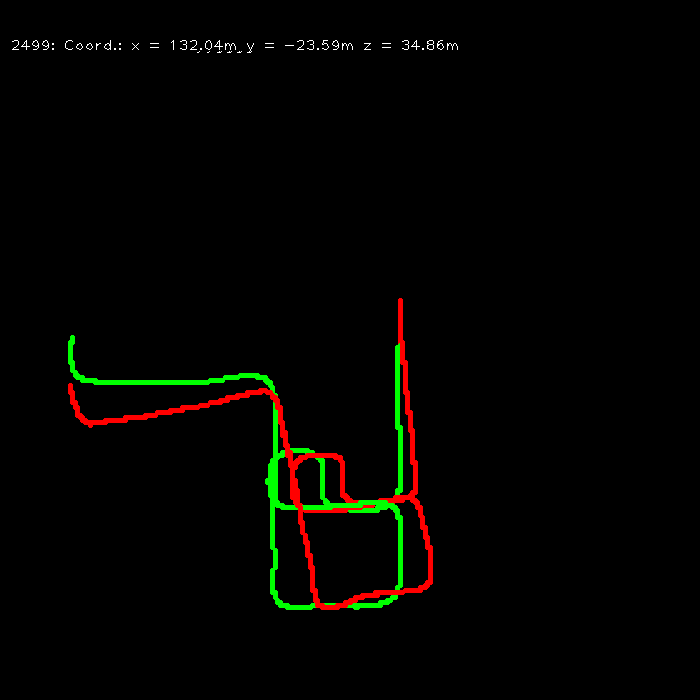
\includegraphics[width=0.5\linewidth]{chapter06/odo/jonas_flexion_AKAZE.png}
    \caption{Flexion image with AKAZE as basis for odometry}
\end{figure}

\subsection{Keypoint Detector Discussion}

The presented results for the different state-of-the-art keypoint detectors imply that good performance on classical camera footage does not automatically yield good performance in the proposed feature images.
Detectors that solely work on corner detection, as \acrshort{orb} does with \acrshort{fast} or the Harris-Corner-Detector, have a hard time on the feature images.
The experiments on real sensor data show, that they strongly respond to missing measurements, that create a sharp black to gray edge.
Solely relying on such areas is unstable and undesirable.
Flat out banning such keypoints on the other hand might not be the right choice either.
Shadow effects and reflective properties of surfaces can produce missing range values, too.
Areas with such consistent black patches can and should be exploited as feature.

\acrshort{surf}'s results are the most surprising, especially in comparison to \acrshort{sift}.
\acrshort{surf} is designed as a faster \acrshort{sift}, using the same principles and underlying theory.
One reason for the bad results might be too many simplifications and approximations.
The use of a box-filter compared to a Gaussian in combination with the other assumptions are justified with empirical analysis on colored images.
In these cases \acrshort{surf} performs good enough, but the bigger deviation from the theoretical background and human perception compared to \acrshort{sift} seem to hurt effectiveness in the novel feature images.
After all, \acrshort{surf} does find true correspondences in some instances.

\acrshort{sift} and \acrshort{akaze} provide the most effective keypoint detectors tested.
\acrshort{akaze}'s keypoint sizes are not as diverse as \acrshort{sift}'s, but the absolute number of keypoints is a clear advantage for example visual odometry tasks.
The surprisingly low number of \acrshort{akaze} keypoints in the \emph{Laserscan} (Appendix~\ref{sec:backprojection_akaze}) could be due to a bad implementation regarding image scaling of very wide images.
This effect requires further research.

\subsection{Feature-Descriptor Discussion}

\acrshort{sift} again proves as a very good descriptor that has over 80\% recall in even challenging conditions.
This unmet performance comes at the cost of high computational complexity and memory footprint, simply recreating some of the reasons why alternatives to \acrshort{sift} were developed in classical computer vision.
Still, for global place recognition, loop closure and other tasks requiring such descriptive power, \acrshort{sift} seems to be the first choice for the feature images.
The odometry results are a clear indication, that \acrshort{sift}'s keypoint detector does not produce enough features, at least for classical pinhole cameras and geometrically clean looking scenes.

The very similar descriptor \acrshort{mldb} and \acrshort{brief}, used in \acrshort{akaze} and \acrshort{orb} respectively, proof their potential, too.
They function very different compared to \acrshort{sift}'s brightness histograms.
The brightness sampling around the keypoint and construction of the binary descriptor is effective.
Using an averaged value for the area around the sampling point improves the robustness of \acrshort{mldb}.
The combination of \acrshort{sift} keypoint detector and descriptor has a slightly lower false positive rate compared to \acrshort{akaze}'s detector and \acrshort{mldb}, but the difference in the number of keypoints needs to be considered, too.
The much lesser computational complexity and drastically higher matching speed of \acrshort{mldb} is promising for real-time applications, like visual odometry.

The Haar-Wavelet response-based descriptor \acrshort{surf} falls flat for both \glspl{flexion-image} and \glspl{bearing-angle-image}.
Similar to the \acrshort{fast} detector, the lack of strong edges typically induced by texture in color images seems to be the main reason for this shortcoming.
Another indication for this finding is, that \acrshort{kaze} has similar Random-Guess perfomance like \acrshort{surf}.
\acrshort{kaze}'s descriptor is not discussed further, but part of the \acrshort{akaze} tests and is based on the \acrshort{surf} descriptor.

It is interesting to see, that the false positive rate is around 35\%$\pm$5\% for all evaluated descriptors.
This can be partly explained by inherent similarity of objects in the scenes.
As only the geometric shape serves as information source, similarity between boxes and edges will always exist.
The more nuanced shading details, complex textures and color differences from color images can not influence the result.
An additional factor to such a similar false positive rate is the rudimentary matching scheme applied.
A reasonable maximum matching distance and additional heuristics in the matching system will produce less false positives.
Such heuristics do not exist yet for the proposed feature images and only this evaluation brings an empirical foundation for such heuristics.

\subsection{Error Discussion}

\begin{itemize}
    \item Sensor noise
    \item Missing Sensordata in combination with noise gives bad flexion images
\end{itemize}

\newpage

\section{Conclusion}

Very Sensors dependent, Time-of-flight and Laserscan gives the best quality.
SURF does not perform well, Bearing Angle gives lower response and less stability
Flexion is very nice.
FAST based stuff does not perform well, more exotic descriptors neither.
SIFT best, AKAZE very good.
Approach to transform depth image first before processing further works and gives results.

\subsection{Future Work}

The proposed \gls{flexion-image} bridges the gap between pointcloud processing and classical computer vision algorithms.
Common processes, as visual odometry, global localisation with a bag-of-words approach and maybe even optical flow algorithms should be evaluated.
The foundational insights on the descriptor performance of \acrshort{sift} and \acrshort{akaze} help to finetune heuristics, such as the maximum matching distance, for these tasks.

New formulations for visual odometry and relative pose calculation become possible, because the range value for each pixel is available.
This additional information for each image coordinate reduces the required number of true correspondences to reconstruct the relative pose.
Investigating the viability of a new formulation for this problem and potential speed and efficiency gains seems to be the highest value research targets.
The classical \acrshort{icp} formulation relies on establishing explicit correspondences between points, too.
Using the \gls{flexion-image} and classical feature descriptors might result in a new variation of this algorithm.
Both problems are related and need further research.

\newpage

\begin{appendix}
    % \clearpage
    \renewcommand*{\thepage}{\thesection\arabic{page}}
    \renewcommand{\thetable}{\thesection\arabic{table}}
    \renewcommand{\thefigure}{\thesection\arabic{figure}}

    % \input{anhang/content}
    \newpage

    \section{Derivation of Formulae}
    \subsection{Bearing-Angle Formula}\label{sec:bearing_derivation}

This section provides the exact derivation of the \gls{bearing-angle} formula.
The literature on \gls{bearing-angle} disagrees on the formula and have mathematical errors.
The full chain of derivation and graphical presentations goal is to provide a trustworthy and checkable background for the provided formula.

\begin{figure}[H]
    \tikzset{every picture/.style={line width=0.75pt}} %set default line width to 0.75pt        
\begin{tikzpicture}[x=0.75pt,y=0.75pt,yscale=-1,xscale=1]
    %uncomment if require: \path (0,341); %set diagram left start at 0, and has height of 341

    %Straight Lines [id:da6739847496898159] 
    \draw  [dash pattern={on 0.84pt off 2.51pt}]  (122.83,145.01) -- (252.88,82) ;
    %Shape: Arc [id:dp4878212457791631] 
    \draw  [draw opacity=0] (240.62,116.61) .. controls (227.55,113.98) and (217.71,102.44) .. (217.71,88.6) .. controls (217.71,82.88) and (219.39,77.55) .. (222.28,73.08) -- (246.29,88.6) -- cycle ; \draw  [color={rgb, 255:red, 208; green, 2; blue, 27 }  ,draw opacity=1 ] (240.62,116.61) .. controls (227.55,113.98) and (217.71,102.44) .. (217.71,88.6) .. controls (217.71,82.88) and (219.39,77.55) .. (222.28,73.08) ;
    %Shape: Arc [id:dp901574933751006] 
    \draw  [draw opacity=0] (113.13,44.58) .. controls (112.48,59.91) and (102.88,72.93) .. (89.43,78.54) -- (74.58,42.92) -- cycle ; \draw  [color={rgb, 255:red, 74; green, 144; blue, 226 }  ,draw opacity=1 ] (113.13,44.58) .. controls (112.48,59.91) and (102.88,72.93) .. (89.43,78.54) ;
    %Shape: Polygon [id:ds6190617836836185] 
    \draw   (67.51,32.91) -- (255.81,82) -- (178.15,257.12) -- cycle ;
    %Shape: Ellipse [id:dp4849771561113211] 
    \draw  [fill={rgb, 255:red, 0; green, 0; blue, 0 }  ,fill opacity=1 ] (251.95,82) .. controls (251.95,80.38) and (253.26,79.07) .. (254.88,79.07) .. controls (256.5,79.07) and (257.81,80.38) .. (257.81,82) .. controls (257.81,83.62) and (256.5,84.93) .. (254.88,84.93) .. controls (253.26,84.93) and (251.95,83.62) .. (251.95,82) -- cycle ;
    %Shape: Circle [id:dp8356396848663105] 
    \draw  [fill={rgb, 255:red, 0; green, 0; blue, 0 }  ,fill opacity=1 ] (64.58,32.84) .. controls (64.58,31.22) and (65.89,29.91) .. (67.51,29.91) .. controls (69.13,29.91) and (70.44,31.22) .. (70.44,32.84) .. controls (70.44,34.46) and (69.13,35.77) .. (67.51,35.77) .. controls (65.89,35.77) and (64.58,34.46) .. (64.58,32.84) -- cycle ;
    %Shape: Arc [id:dp8012007227541399] 
    \draw  [draw opacity=0] (157.23,215.86) .. controls (163.51,212.67) and (170.62,210.87) .. (178.15,210.87) .. controls (184.79,210.87) and (191.12,212.27) .. (196.83,214.8) -- (178.15,257.12) -- cycle ; \draw   (157.23,215.86) .. controls (163.51,212.67) and (170.62,210.87) .. (178.15,210.87) .. controls (184.79,210.87) and (191.12,212.27) .. (196.83,214.8) ;
    %Shape: Right Angle [id:dp07010543377164635] 
    \draw   (116.98,132.65) -- (129.04,126.95) -- (134.88,139.31) ;

    % Text Node
    \draw (161.42,39.19) node [anchor=north west][inner sep=0.75pt]   [align=left] {$\displaystyle a$};
    % Text Node
    \draw (159.22,106.59) node [anchor=north west][inner sep=0.75pt]   [align=left] {$\displaystyle h$};
    % Text Node
    \draw (230.37,145.44) node [anchor=north west][inner sep=0.75pt]   [align=left] {$\displaystyle d_{i}$};
    % Text Node
    \draw (93.81,147.37) node [anchor=north west][inner sep=0.75pt]   [align=left] {$\displaystyle d_{i-1}$};
    % Text Node
    \draw (168.08,216.65) node [anchor=north west][inner sep=0.75pt]   [align=left] {$\displaystyle d\varphi $};
    % Text Node
    \draw (230.1,90.96) node [anchor=north west][inner sep=0.75pt]  [color={rgb, 255:red, 208; green, 2; blue, 27 }  ,opacity=1 ] [align=left] {$\displaystyle \beta $};
    % Text Node
    \draw (87.69,51.2) node [anchor=north west][inner sep=0.75pt]  [color={rgb, 255:red, 74; green, 144; blue, 226 }  ,opacity=1 ] [align=left] {$\displaystyle \gamma $};
    % Text Node
    \draw (101.34,84.61) node [anchor=north west][inner sep=0.75pt]   [align=left] {$\displaystyle b$};
    % Text Node
    \draw (144.57,170.34) node [anchor=north west][inner sep=0.75pt]   [align=left] {$\displaystyle c$};
    % Text Node
    \draw (169.08,261.2) node [anchor=north west][inner sep=0.75pt]   [align=left] {$\displaystyle \mathbf{C}$};
    % Text Node
    \draw (261,72.76) node [anchor=north west][inner sep=0.75pt]   [align=left] {$\displaystyle \mathbf{P}_{i}$};
    % Text Node
    \draw (28.06,27.4) node [anchor=north west][inner sep=0.75pt]   [align=left] {$\displaystyle \mathbf{P}_{i-1}$};
\end{tikzpicture}

    \caption[Derivation of the \gls{bearing-angle} with all support variables]{\emph{Derivation of the \gls{bearing-angle} with all support variables.} Deriving the bearing angle requires additional support variables that are introduced with this figure. Using fundamental trigonometry allows derivation of the formula.}\label{fig:bearing-derivation}
\end{figure}

The cosine theorem holds true for all triangles and is the central equality for the derivation.
\begin{equation}
\begin{aligned}
    \text{Ansatz:} \\
    d_{i-1}^2 &= d_i^2 + a^2 - 2 d_i a \cos \beta \qquad \text{(Cosine Theorem)} \\
\end{aligned}
\end{equation}
Introducing supporting variables at the positions given in Figure~\ref{fig:bearing-derivation} allows substiting the missing quantity $a$.
\begin{equation*}
\begin{aligned}
    h &= d_i \sin d\varphi \\
    c &= d_i \cos d\varphi \\
    b &= d_{i-1} - d_i \cos d\varphi \\
    a^2 &= h^2 + b^2 \\
    a^2 &= \mathunderline{darkgreen}{(d_i \sin d\varphi)^2} + \mathunderline{plotblue}{(d_{i-1} - d_i \cos d\varphi)^2} \\
    a^2 &= \mathunderline{darkgreen}{\mathunderline{darkred}{d_i^2 \sin^2 d\varphi}} +
           \mathunderline{plotblue}{%
             \mathunderline{plotorange}{d_{i-1}^2 - 2 d_{i-1} d_i \cos d\varphi} +
             \mathunderline{darkred}{d_i^2 \cos^2 d\varphi}
           } \\
    a^2 &= \mathunderline{darkred}{d_{i-1}^2 \sin^2 d\varphi + d_{i-i}^2 \cos^2 d\varphi} +
           \mathunderline{plotorange}{d_{i-1}^2 -2 d_{i-1} d_i \cos d\varphi} \\
    a^2 &= \mathunderline{darkred}{d_i^2} +
           \mathunderline{plotorange}{d_{i-1}^2 - 2 d_{i-1} d_i \cos d\varphi} \\
\end{aligned}
\end{equation*}
For $a$ holds the condition $a > 0$ for all values, because the constraints $d_i > 0$, $d_{i-1} > 0$ and $0 < d\varphi < \pi$ result from the properties of depth sensors.

The variable $a$ is now substituted in the ansatz.
Consequent simplification of the equations yields the final formula for the bearing angle.
\begin{equation*}
\begin{aligned}
    d_{i-1}^2 &= d_i^2 + a^2 - 2 d_i a \cos \beta \\
    \mathunderline{plotblue}{d_{i-1}^2} &= \mathunderline{darkred}{d_i^2} +
    \mathunderline{darkred}{d_i^2} + \mathunderline{plotblue}{d_{i-1}^2} - 2 d_{i-1} d_i \cos d\varphi
    - 2 d_i \sqrt{d_i^2 + d_{i-1}^2 -2 d_{i-1} d_i \cos d\varphi} \cos \beta \\
    \mathunderline{plotblue}{0} &= \mathunderline{darkgreen}{2} \mathunderline{darkred}{d_i^2} +
                                   \mathunderline{plotblue}{0} -
                                   \mathunderline{darkgreen}{2} \mathunderline{darkred}{d_{i-1}} d_i \cos d\varphi
                                   - \mathunderline{darkgreen}{2} \mathunderline{darkred}{d_i} \sqrt{d_i^2 + d_{i-1}^2 -2 d_{i-1} d_i \cos d\varphi} \cos \beta \\
   0 &= \mathunderline{darkred}{d_i^2} - \mathunderline{darkred}{d_{i}} d_{i-1} \cos d\varphi
       - \mathunderline{darkred}{d_i} \sqrt{d_i^2 + d_{i-1}^2 -2 d_{i-1} d_i \cos d\varphi} \cos \beta \\
   0 &= \mathunderline{darkred}{d_i} - \mathunderline{darkred}{1} d_{i-1} \cos d\varphi
       - \mathunderline{darkred}{1} \sqrt{d_i^2 + d_{i-1}^2 -2 d_{i-1} d_i \cos d\varphi} \cos \beta \\
   \cos \beta &= \frac{d_i - d_{i-1} \cos d\varphi}{\sqrt{d_i^2 + d_{i-1}^2 -2 d_{i-1} d_i \cos d\varphi}} \\
   \beta &= \arccos \frac{d_i - d_{i-1} \cos d\varphi}{\sqrt{d_i^2 + d_{i-1}^2 -2 d_{i-1} d_i \cos d\varphi}} \\
\end{aligned}
\end{equation*}

% vim: set nocindent nosmartindent


    \newpage

    \addcontentsline{toc}{section}{References}
    \bibliographystyle{IEEEtran}
    \bibliography{references}

    \newpage
    \addcontentsline{toc}{section}{\listtablename}\listoftables

    \newpage
    \addcontentsline{toc}{section}{\listfigurename}\listoffigures

    \newpage
    %\renewcommand{\indexname}{Stichwortverzeichnis}
    %\addcontentsline{toc}{section}{Stichwortverzeichnis}
    % \printindex
\end{appendix}
\end{document}
